\documentclass[12pt]{article}
\usepackage[table]{xcolor}
\usepackage{amsmath, bm, bbm}
\usepackage{amssymb, amsthm, graphicx}
\usepackage{enumitem}
%\usepackage{color}
\usepackage{float}
\usepackage{rotating}
\usepackage[small]{caption}
\usepackage{subcaption}
\usepackage[mathscr]{euscript}
\usepackage{dsfont}
\usepackage{natbib}
\usepackage{amsmath}
\usepackage{placeins}
\usepackage{rotating, tabularx}
\usepackage{booktabs}
\usepackage{pdflscape}
\makeatletter
\renewcommand{\eqref}[1]{\tagform@{\ref{#1}}}
\def\maketag@@@#1{\hbox{#1}}
\makeatother
\usepackage{bibentry}
\usepackage[hang,flushmargin]{footmisc} 
\usepackage{setspace}
\usepackage{titlesec}
\titlespacing*{\section}{0pt}{5pt}{5pt}
\titlespacing*{\subsection}{0pt}{5pt}{5pt}
\parindent0pt

%\pdfminorversion=4
% NOTE: To produce blinded version, replace "0" with "1" below.
\newcommand{\blind}{0}

% DON'T change margins - should be 1 inch all around.
\addtolength{\oddsidemargin}{-.5in}%
\addtolength{\evensidemargin}{-1in}%
\addtolength{\textwidth}{1in}%
\addtolength{\textheight}{1.7in}%
\addtolength{\topmargin}{-1in}%


% General

\newcommand{\reals}{\mathbb{R}}
\newcommand{\integers}{\mathbb{Z}}
\newcommand{\naturals}{\mathbb{N}}

\newcommand{\pr}{\mathbb{P}}        % probability
\newcommand{\ex}{\mathbb{E}}        % expectation
\newcommand{\var}{\textnormal{Var}} % variance
\newcommand{\cov}{\textnormal{Cov}} % covariance

\newcommand{\law}{\mathcal{L}} % law of X
\newcommand{\normal}{N}        % normal distribution 

\newcommand{\argmax}{\textnormal{argmax}}
\newcommand{\argmin}{\textnormal{argmin}}

\newcommand{\ind}{\mathbbm{1}} % indicator function
\newcommand{\kernel}{K} % kernel function
\newcommand{\wght}{W} % kernel weight
\newcommand{\thres}{\pi} % threshold parameter


% Convergence

\newcommand{\convd}{\stackrel{d}{\longrightarrow}}              % convergence in distribution
\newcommand{\convp}{\stackrel{P}{\longrightarrow}}              % convergence in probability
\newcommand{\convas}{\stackrel{\textrm{a.s.}}{\longrightarrow}} % convergence almost surely
\newcommand{\convw}{\rightsquigarrow}                           % weak convergence


% Theorem-like declarations

\theoremstyle{plain}

\newtheorem{theorem}{Theorem}[section]
\newtheorem{prop}[theorem]{Proposition}
\newtheorem{lemma}[theorem]{Lemma}
\newtheorem{corollary}[theorem]{Corollary}
\newtheorem*{theo}{Theorem}
\newtheorem{propA}{Proposition}[section]
\newtheorem{lemmaA}[propA]{Lemma}
\newtheorem{definition}{Definition}[section]
\newtheorem{remark}{Remark}[section]
\renewcommand{\thelemmaA}{A.\arabic{lemmaA}}
\renewcommand{\thepropA}{A.\arabic{propA}}
\newtheorem*{algo}{Clustering Algorithm}


% Theorem numbering to the left

\makeatletter
\newcommand{\lefteqno}{\let\veqno\@@leqno}
\makeatother


% Heading

\newcommand{\heading}[2]
{  \setcounter{page}{1}
   \begin{center}

   \phantom{Distance to upper boundary}
   \vspace{0.5cm}

   {\LARGE \textbf{#1}}
   \vspace{0.4cm}
 
   {\LARGE \textbf{#2}}
   \end{center}
}


% Authors

\newcommand{\authors}[4]
{  \parindent0pt
   \begin{center}
      \begin{minipage}[c][2cm][c]{5cm}
      \begin{center} 
      {\large #1} 
      \vspace{0.05cm}
      
      #2 
      \end{center}
      \end{minipage}
      \begin{minipage}[c][2cm][c]{5cm}
      \begin{center} 
      {\large #3}
      \vspace{0.05cm}

      #4 
      \end{center}
      \end{minipage}
   \end{center}
}

%\newcommand{\authors}[2]
%{  \parindent0pt
%   \begin{center}
%   {\large #1} 
%   \vspace{0.1cm}
%      
%   #2 
%   \end{center}  
%}


% Version

\newcommand{\version}[1]
{  \begin{center}
   {\large #1}
   \end{center}
   \vspace{3pt}
} 








\usepackage{xr}
\externaldocument{paper}

%\usepackage{hyperref}



\begin{document}

\def\spacingset#1{\renewcommand{\baselinestretch}%
{#1}\small\normalsize} \spacingset{1}

\headingSupplement{Supplement to}{``Multiscale Comparison}{of Nonparametric Trend Curves''}
%\authors{Marina Khismatullina}{Erasmus University Rotterdam}{Michael Vogt}{Ulm University} 

%\renewcommand{\abstractname}{}
%\begin{abstract}
%\end{abstract}

\spacingset{1.8} % DON'T change the spacing!

\def\thesection{\Alph{section}}

\numberwithin{equation}{section}
\numberwithin{figure}{section}
\numberwithin{table}{section}
\allowdisplaybreaks[4]

\setlength{\abovedisplayskip}{3pt}
\setlength{\belowdisplayskip}{3pt}



\section{Simulations}\label{sec:sim}


In this section, we investigate our test and clustering methods by means of Monte Carlo experiments.


\subsection{Size and power of the multiscale test}\label{subsec:sim:main} 


The simulation design is as follows: We generate data from the model $Y_{it} = m_i(\frac{t}{T}) + \bfbeta_i^\top \X_{it} +  \alpha_i  + \varepsilon_{it}$, where the number of time series is set to $n = 15$ and we consider different time series lengths $T$. We include $3$ covariates and model them by the VAR(3) process
\[ \boldsymbol{X}_{it} = \begin{pmatrix} a_1 & 0 & 0 \\ 0 & a_2 & 0 \\ 0 & 0 & a_3 \end{pmatrix} \boldsymbol{X}_{i,t-1} + \boldsymbol{\nu}_{it}, \] 
where $\boldsymbol{X}_{it} = ( X_{it,1}, X_{it,2}, X_{it,3} )^\top$, $\boldsymbol{\nu}_{it} = ( \nu_{it,1}, \nu_{it,2}, \nu_{it,3} )^\top$ and we choose $a_1 = a_2 = a_3 = 0.25$. The innovations $\boldsymbol{\nu}_{it}$ are drawn i.i.d.\ from a multivariate normal distribution $N(0,\Phi)$ with
\[ \Phi = \begin{pmatrix} 1 & \varphi & \varphi \\ \varphi & 1 & \varphi \\ \varphi & \varphi & 1 \end{pmatrix}, \]
where $\varphi = 0.25$\footnote{We have repeated the analysis for $\phi = 0.1$ and the results are roughly the same.} specifies the correlation between the 3 covariates. The parameter vector $\boldsymbol{\beta}_i = (\beta_{i,1},\beta_{i,2},\beta_{i,3})^\top$ is chosen to equal $(1,1,1)^\top$ for each $i$. Moreover, for each $i$, the idiosyncratic error process $\{\varepsilon_{it}: 1 \le t \le T\}$ follows the AR(1) model $\varepsilon_{it} = a \varepsilon_{i, t-1} + \eta_{it}$, where $a = 0.25$ and the innovations $\eta_{it}$ are i.i.d.\ normally distributed with mean $0$ and standard deviation $0.25$. 
The vector of fixed effects $\boldsymbol{\alpha} = (\alpha_1,\ldots,\alpha_n)^\top$ is modelled as a normally distributed random vector. In particular, $\boldsymbol{\alpha} \sim N(0,\Sigma)$ with
\[ \Sigma =
\begin{pmatrix}
1      & \rho   & \cdots & \rho   \\
\rho   & 1      & \ddots & \vdots \\
\vdots & \ddots & \ddots & \rho   \\
\rho   & \cdots & \rho   & 1
\end{pmatrix},
\]
where $\rho = 0.25$\footnote{We have repeated the analysis for $\rho = 0.1$ and the results are roughly the same.} gives the correlation across $i$.
%We assume that the covariates $\X_{it}$ and the error terms $\varepsilon_{js}$ are independent from each other for all $1 \leq i,j \leq n$ and $1 \leq t, s \leq T$. 
To generate data under the null $H_0: m_1 = \ldots = m_n$, we let $m_i = 0$ for all $i$ without loss of generality. To produce data under the alternative, we use the bump function
\begin{align}
m_1(u) =  b \cdot  \vartheta(u, 0.3, 0.1) - b  \cdot  \vartheta(u,0.7, 0.1)  \label{eq:bump-fct}
\end{align}

with $\vartheta(u,c,d) =  \ind\left\{\frac{|u - c|}{d}\leq 1\right\} \left(1 - \frac{(u - c)^2}{d^2}\right)^2$ for $b \in \{ 0.25, 0.5, 0.75 \}$ (depicted in Figure \ref{fig:bump_function}) and let $m_i = 0$ for $i \neq 1$. Note that the normalisation constraint $\int_0^1 m_1(u) du = 0$ is directly satisfied in this case. For each simulation exercise, we draw $5000$ samples.


\begin{figure}[t!]
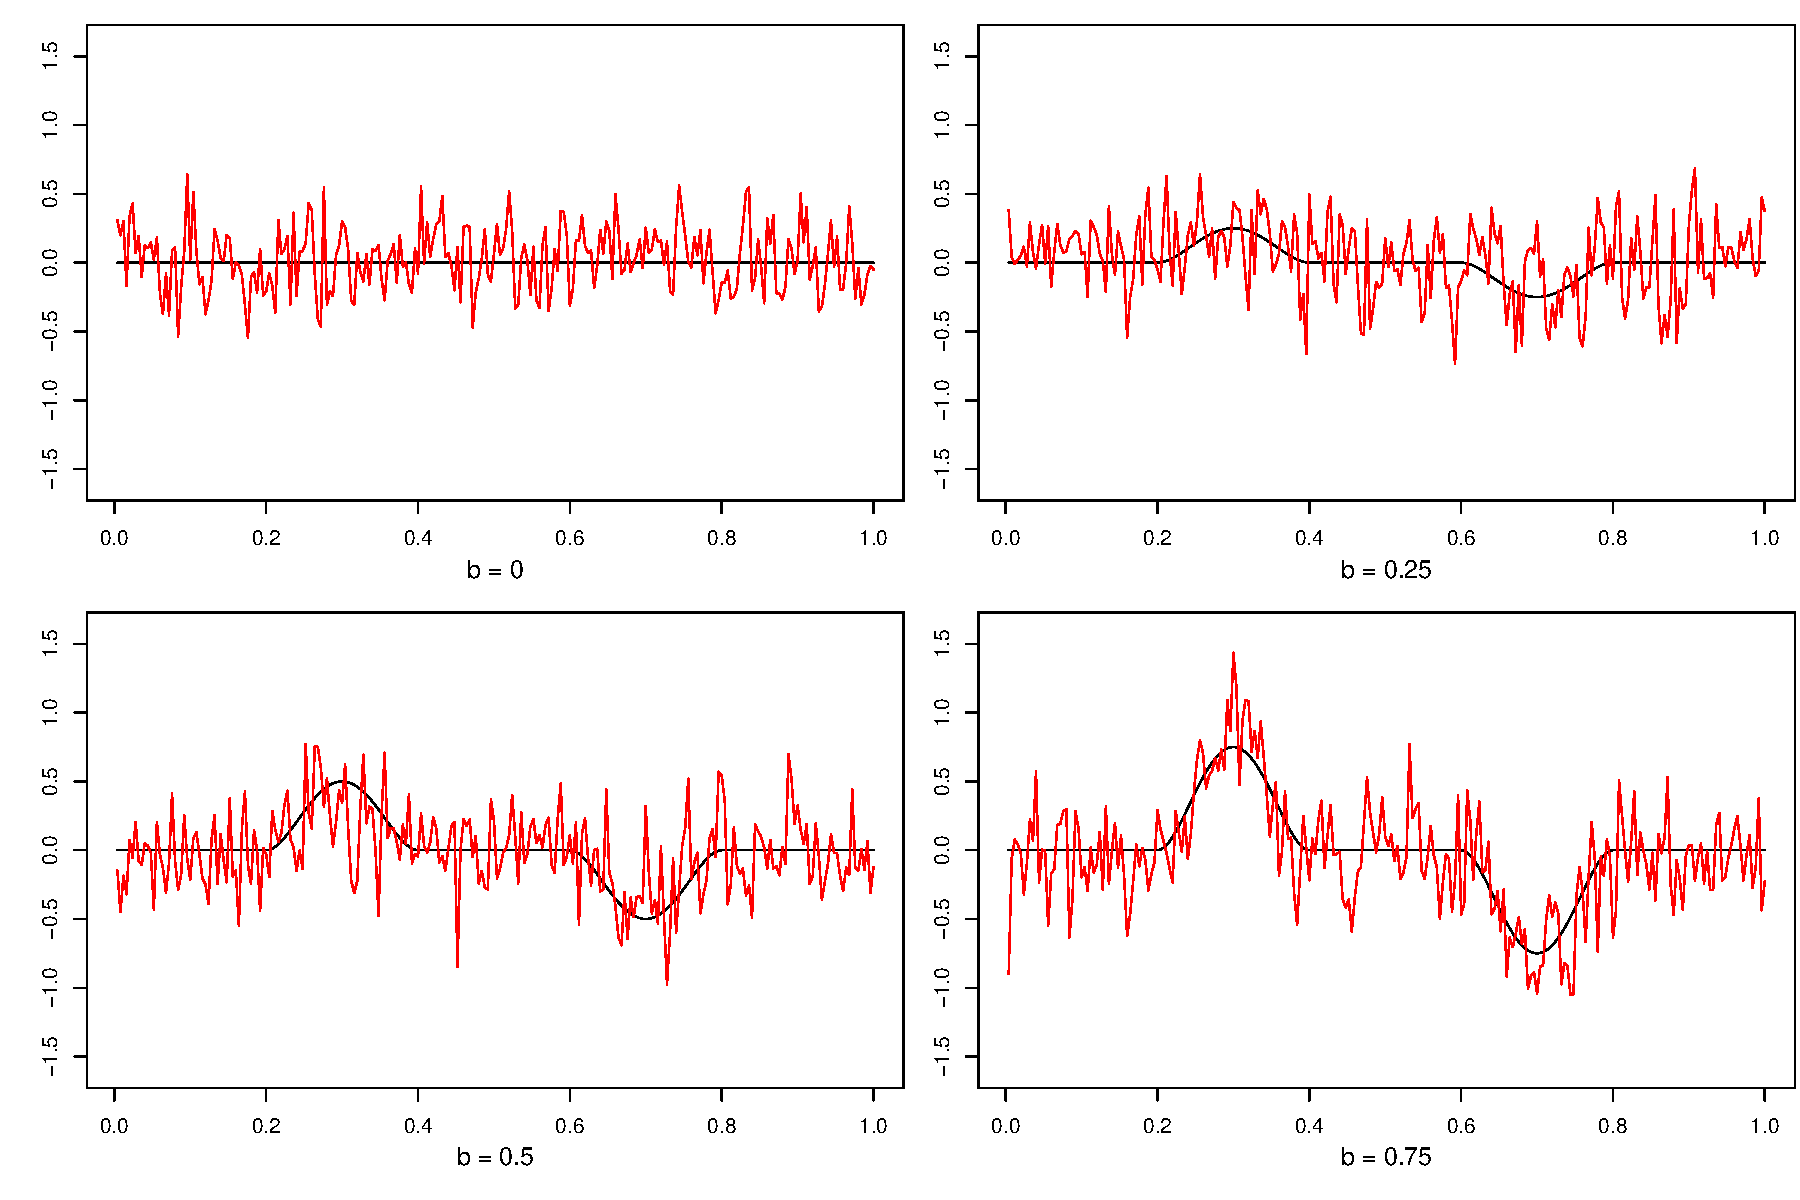
\includegraphics[width=\textwidth]{../output/bump_function.pdf}
\caption{In black: the bump function $m_1$ for different bump heights $b \in \{0, 0.25, 0.5, 0.75\}$ with $b=0$ corresponding to the null $H_0$. In red: the time series $\{Y_{1t}^\circ : 1 \le t \le T \}$ with $Y_{1t}^\circ = m_1(t/T) + \varepsilon_{1t}$ for one simulation run and $T=250$.}\label{fig:bump_function}
\end{figure}


Figure \ref{fig:bump_function} illustrates that the described simulation setup is quite challenging already without covariates and fixed effects. The black lines in the plot show the bump function $m_1$ for different heights of the bump $b \in \{0, 0.25, 0.5, 0.75\}$, where the value $b=0$ corresponds to the null $H_0$. The red lines show one realization of the time series $\{Y_{1t}^\circ:1 \le t \le T \}$ for $T=250$, where $Y_{1t}^\circ = m_1(\frac{t}{T}) + \varepsilon_{1t}$ is an idealized version of $Y_{1t}$ without covariates and fixed effects. The values $b=0.25,0.5,0.75$ correspond to three different alternatives. In particular, the larger the bump size $b$, the further away from the null is the corresponding alternative. For the smallest value $b=0.25$, the bump function is very difficult to detect since the noise level is very high, or put differently, since the signal-to-noise ratio is very small (as is clearly visible in the upper right panel of Figure \ref{fig:bump_function}). For $b=0.5$ and $b=0.75$, the signal-to-noise ratio slowly gets bigger, making it less difficult to detect the bump function. Nevertheless, even for $b=0.75$, there is substantial noise around the bump function, meaning that detection of the bump is still non-trivial. 


Our multiscale test is implemented as follows: The estimators $\widehat{\bfbeta}_i$ and $\widehat{\alpha}_i$ of the unknown parameters $\bfbeta_i$ and $\alpha_i$ are computed as described in Section~\ref{subsec:test:prep}. Since the errors $\varepsilon_{it}$ follow an AR($1$) process, we estimate the long-run error variance by the difference-based estimator proposed in \cite{KhismatullinaVogt2020}, setting the tuning parameters $q$ and $r$ to $25$ and $10$, respectively. In order to construct our test statistics, we use an Epanechnikov kernel and the grid $\mathcal{G}_T = U_T \times H_T$ with
\begin{align}
U_T & = \big\{ u \in [0,1]: u = \textstyle{\frac{5t}{T}} \text{ with } 1 \le t \le T \big\} \label{eq:grid-loc} \\
H_T & = \big\{ h \in \big[ \textstyle{\frac{\log T}{T}}, \textstyle{\frac{1}{4}} \big]:  h = \textstyle{\frac{5 t -3}{T}} \text{ with } 1 \le t \le T \big\}. \label{eq:grid-scale}
\end{align}
We thus consider intervals $\mathcal{I}_{u, h} = [u-h, u+h]$ which contain $5, 15, 25, \ldots$ data points. The critical value $q_{n,T}(\alpha)$ of our test is computed by Monte Carlo methods as described in Section \ref{subsec:test:impl}, where we set $L=5000$. 


\begin{table}[t!]
\renewcommand{\arraystretch}{1.2}  
\footnotesize{
\begin{center}
\caption{Empirical size and power of the multiscale test for different sample sizes $T$ and nominal sizes $\alpha$.
Each panel gives the results for a different bump height $b$, where $b = 0$ corresponds to the null and $b = 0.25,0.5,0.75$ to three different alternatives.}\label{tab:sizepower}
\begin{subtable}[b]{0.4\textwidth}
\centering  
\caption{$b=0$}
% latex table generated in R 4.3.1 by xtable 1.8-4 package
% 
\begin{tabular}{cccc}
  \hline
  & \multicolumn{3}{c}{nominal size $\alpha$} \\
 $T$ & 0.01 & 0.05 & 0.1 \\
 \hline
100 & 0.008 & 0.039 & 0.085 \\ 
  250 & 0.018 & 0.072 & 0.118 \\ 
  500 & 0.014 & 0.070 & 0.124 \\ 
   \hline
\end{tabular}
%This simulation was done for the seed 111333555, for the following values of the parameters: n_ts = 15, with 5000 simulations for calculating size and power and 5000 simulations to calculate the Gaussian quantiles. Furthermore, for the error process we have a = 0.25 and sigma = 0.25. For the covariate process a_1 = a_2 = a_3 = 0.25 and phi = 0.25. For the fixed effect, we have rho = 0.25. The grid is fine (growing with the sample size)

\end{subtable}
\begin{subtable}[b]{0.4\textwidth}
\centering  
\caption{$b=0.25$}
% latex table generated in R 4.3.1 by xtable 1.8-4 package
% 
\begin{tabular}{cccc}
  \hline
  & \multicolumn{3}{c}{nominal size $\alpha$} \\
 $T$ & 0.01 & 0.05 & 0.1 \\
 \hline
100 & 0.013 & 0.056 & 0.109 \\ 
  250 & 0.054 & 0.156 & 0.250 \\ 
  500 & 0.157 & 0.373 & 0.497 \\ 
   \hline
\end{tabular}
%This simulation was done for the following values of the parameters: n_ts = 15, with 5000 simulations for calculating size and power and 5000 simulations to calculate the Gaussian quantiles. Furthermore, for the error process we have a = 0.25 and sigma = 0.25. For the covariate process a_1 = a_2 = a_3 = 0.25 and phi = 0.25. For the fixed effect, we have rho = 0.25. The grid is fine (growing with the sample size)

\end{subtable}
\begin{subtable}[b]{0.4\textwidth}
\centering  
\vspace{0.25cm} \caption{$b=0.5$}
% latex table generated in R 4.3.1 by xtable 1.8-4 package
% 
\begin{tabular}{cccc}
  \hline
  & \multicolumn{3}{c}{nominal size $\alpha$} \\
 $T$ & 0.01 & 0.05 & 0.1 \\
 \hline
100 & 0.012 & 0.051 & 0.101 \\ 
  250 & 0.844 & 0.955 & 0.980 \\ 
  500 & 1.000 & 1.000 & 1.000 \\ 
   \hline
\end{tabular}
%This simulation was done for the seed 22446688, for the following values of the parameters: n_ts = 15, with 5000 simulations for calculating size and power and 5000 simulations to calculate the Gaussian quantiles. Furthermore, for the error process we have a = 0.25 and sigma = 0.25. For the covariate process a_1 = a_2 = a_3 = 0.25 and phi = 0.25. For the fixed effect, we have rho = 0.25. The grid is fine (growing with the sample size)

\end{subtable}
\begin{subtable}[b]{0.4\textwidth}
\centering  
\vspace{0.25cm} \caption{$b=0.75$}
% latex table generated in R 4.3.1 by xtable 1.8-4 package
% 
\begin{tabular}{cccc}
  \hline
  & \multicolumn{3}{c}{nominal size $\alpha$} \\
 $T$ & 0.01 & 0.05 & 0.1 \\
 \hline
100 & 0.005 & 0.030 & 0.066 \\ 
  250 & 0.966 & 0.993 & 0.996 \\ 
  500 & 1.000 & 1.000 & 1.000 \\ 
   \hline
\end{tabular}
%This simulation was done for the seed 22446688, for the following values of the parameters: n_ts = 15, with 5000 simulations for calculating size and power and 5000 simulations to calculate the Gaussian quantiles. Furthermore, for the error process we have a = 0.25 and sigma = 0.25. For the covariate process a_1 = a_2 = a_3 = 0.25 and phi = 0.25. For the fixed effect, we have rho = 0.25. The grid is fine (growing with the sample size)

\end{subtable}
\end{center}}
\end{table}


Table \ref{tab:sizepower} reports the simulation results, in particular, the empirical size and power of the multiscale test. Both the empirical size and the empirical power are computed as the number of simulations in which the test rejects the global null $H_0$ divided by the total number of simulations.
%The left column of Table \ref{tab:sizepower} gives the results for the simulation setting with the correlation parameters $(\phi,\rho) = (0.1,0.1)$, the right column those for the setting with $(\phi,\rho) = (0.25,0.25)$. (We do not present the results for $(\phi,\rho) = (0.1,0.25)$ and $(\phi,\rho) = (0.25,0.1)$ as they are quite similar and do not bring additional insights.)
The four panels (a)--(d) of Table \ref{tab:sizepower} correspond to different values of the bump size $b$. Panel (a) corresponds to the case $b=0$ and thus gives the empirical size of the test under the null $H_0$. Panels (b)--(d), in contrast, report the empirical power against the three alternatives with $b \in \{0.25,0.5,0.75\}$.
%The actual size of the test is reported in the two subtables (a), whereas subtables (b)--(d) report the power against the three different alternatives with $b \in \{0.25,0.5,0.75\}$. Both the actual size and the power are computed as the number of simulations in which the test rejects the global null $H_0$ divided by the total number of simulations.
Inspecting panel (a), one can see that the empirical size of the test gives a reasonable approximation to the target $\alpha$ in all scenarios under investigation.
%, even though the size numbers have a slight upward bias. {\color{red}This bias gets smaller as the sample size $T$ increases, which reflects the fact that we get more and more information for each of the tests that we need to carry out.} We can also see that the upward bias become slightly more pronounced in case of stronger degrees of correlation across the covariates and the time series, i.e., with higher values of $\phi$ and $\rho$, but the change in test performance is almost negligible and can be attributed to random sampling. To summarize, even though slightly liberal, the test controls the FWER quite accurately in the simulation settings that we consider.
Inspecting panels (b)--(d), one can further see that the test has good power properties. For the smallest height of the bump function $b = 0.25$ and the smallest time series length $T = 100$, the power is only moderate, reflecting the fact that the alternative with $b = 0.25$ is not very far away from the null. However, as we increase the height $b$ and the sample size $T$, the power increases quickly. For the height value $b = 0.5$ and $T=250$, for instance, we already have power of over $95\%$.


\subsection{Robustness checks on the choice of tuning parameters}\label{subsec:sim:grid}


The main tuning parameter of our method is the grid $\mathcal{G}_T$, which in particular specifies the bandwidths that are taken into account. In order to assess the robustness of our test with respect to the grid, we repeat the simulation exercises from Section \ref{subsec:sim:main} with two different choices of the grid: a sparser and a finer grid than the one used in Section \ref{subsec:sim:main}.
The sparser grid is defined as
\begin{align}
\mathcal{G}_T^{\text{sparse}} = \big\{ (u,h) \subseteq [0,1]: & \ (u,h) = ((2s+1) h, h) \text{ for } s = 0,\ldots,\Big\lfloor \frac{h^ {-1}-1}{2} \Big\rfloor \nonumber \\ & \ \text{and } h \in H_T^{\text{sparse}} \big\} \label{eq:grid-sparse}
\end{align}
with $H_T^{\text{sparse}} = \{ h = 2^k h_{\min} \text{ for } k=0,\ldots,K \}$, where $h_{\min} = \frac{\lceil \log T \rceil}{T}$ and $K$ is such that $2^K h_{\min} \le \frac{1}{4}$, i.e., $K \le \lfloor \log(\frac{T}{4 \lceil \log T \rceil }) \rfloor \frac{1}{\log(2)}$. This is a dyadic scheme with scales in the set $H_T^{\text{sparse}}$ as commonly used in Wavelet analysis. 
The finer grid is defined as
$\mathcal{G}_T^{\text{fine}} = U_T^{\text{fine}} \times H_T^{\text{fine}}$,
where  
$U_T^{\text{fine}}  = \{ u \in [0,1]: u = \textstyle{\frac{t}{T}} \text{ with } 1 \le t \le T \}$
and
$H_T^{\text{fine}} = \{ h \in [ \textstyle{\frac{\log T}{T}}, \textstyle{\frac{1}{4}} ]:  h = \textstyle{\frac{2t}{T}} \text{ with } 1 \le t \le T \}$. Such a fine grid significantly increases the number of tests which also affects the computational time. Hence, to decrease the computational time, for the fine grid we calculate the Gaussian quantile based on $L = 1000$ bootstrap samples and we simulate $1000$ samples for each simulation scenario. Apart from this, we work precisely with the same simulation setup as in Section \ref{subsec:sim:main}.


\begin{table}[t!]
\renewcommand{\arraystretch}{1.2}  
\footnotesize{
\begin{center}
\caption{Empirical size and power of the multiscale test for three different grids. Each column corresponds to a particular choice of grid. Panels (a)--(d) of each column have the same structure as in Figure \ref{tab:sizepower}.}\label{tab:grids}
\begin{subtable}[b]{0.32\textwidth}
\setcounter{subtable}{0}    
\centering  
\caption*{sparser grid $\mathcal{G}_T^{\text{sparse}}$}\vspace{0.1cm} 
\caption{$b=0$}
% latex table generated in R 4.3.1 by xtable 1.8-4 package
% 
\begin{tabular}{cccc}
  \hline
  & \multicolumn{3}{c}{nominal size $\alpha$} \\
 $T$ & 0.01 & 0.05 & 0.1 \\
 \hline
100 & 0.008 & 0.033 & 0.068 \\ 
  250 & 0.012 & 0.060 & 0.105 \\ 
  500 & 0.012 & 0.053 & 0.108 \\ 
   \hline
\end{tabular}
%This simulation was done for the seed 543212345, for the following values of the parameters: n_ts = 15, with 5000 simulations for calculating size and power and 5000 simulations to calculate the Gaussian quantiles. Furthermore, for the error process we have a = 0.25 and sigma = 0.25. For the covariate process a_1 = a_2 = a_3 = 0.25 and phi = 0.25. For the fixed effect, we have rho = 0.25. The grid is DYADIC.
\vspace{0.25cm}
\caption{$b=0.25$}
% latex table generated in R 4.3.1 by xtable 1.8-4 package
% 
\begin{tabular}{cccc}
  \hline
  & \multicolumn{3}{c}{nominal size $\alpha$} \\
 $T$ & 0.01 & 0.05 & 0.1 \\
 \hline
100 & 0.010 & 0.046 & 0.085 \\ 
  250 & 0.070 & 0.176 & 0.263 \\ 
  500 & 0.199 & 0.435 & 0.574 \\ 
   \hline
\end{tabular}
%This simulation was done for the seed 22446688, for the following values of the parameters: n_ts = 15, with 5000 simulations for calculating size and power and 5000 simulations to calculate the Gaussian quantiles. Furthermore, for the error process we have a = 0.25 and sigma = 0.25. For the covariate process a_1 = a_2 = a_3 = 0.25 and phi = 0.25. For the fixed effect, we have rho = 0.25. The grid is DYADIC.
\vspace{0.25cm}
\caption{$b=0.5$}
% latex table generated in R 4.3.1 by xtable 1.8-4 package
% 
\begin{tabular}{cccc}
  \hline
  & \multicolumn{3}{c}{nominal size $\alpha$} \\
 $T$ & 0.01 & 0.05 & 0.1 \\
 \hline
100 & 0.014 & 0.060 & 0.105 \\ 
  250 & 0.455 & 0.689 & 0.796 \\ 
  500 & 0.995 & 0.999 & 1.000 \\ 
   \hline
\end{tabular}
%This simulation was done for the seed 22446688, for the following values of the parameters: n_ts = 15, with 5000 simulations for calculating size and power and 5000 simulations to calculate the Gaussian quantiles. Furthermore, for the error process we have a = 0.25 and sigma = 0.25. For the covariate process a_1 = a_2 = a_3 = 0.25 and phi = 0.25. For the fixed effect, we have rho = 0.25. The grid is dyadic.
\vspace{0.25cm}
\caption{$b=0.75$}
% latex table generated in R 4.3.1 by xtable 1.8-4 package
% 
\begin{tabular}{cccc}
  \hline
  & \multicolumn{3}{c}{nominal size $\alpha$} \\
 $T$ & 0.01 & 0.05 & 0.1 \\
 \hline
100 & 0.007 & 0.029 & 0.066 \\ 
  250 & 0.742 & 0.903 & 0.943 \\ 
  500 & 1.000 & 1.000 & 1.000 \\ 
   \hline
\end{tabular}
%This simulation was done for the seed 543212345, for the following values of the parameters: n_ts = 15, with 5000 simulations for calculating size and power and 5000 simulations to calculate the Gaussian quantiles. Furthermore, for the error process we have a = 0.25 and sigma = 0.25. For the covariate process a_1 = a_2 = a_3 = 0.25 and phi = 0.25. For the fixed effect, we have rho = 0.25. The grid is DYADIC.

\end{subtable}
\begin{subtable}[b]{0.32\textwidth}
\setcounter{subtable}{0}  
\centering  
\caption*{grid $\mathcal{G}_T$ from Section \ref{subsec:sim:main}}\vspace{0.1cm} 
\caption{$b=0$}
% latex table generated in R 4.3.1 by xtable 1.8-4 package
% 
\begin{tabular}{cccc}
  \hline
  & \multicolumn{3}{c}{nominal size $\alpha$} \\
 $T$ & 0.01 & 0.05 & 0.1 \\
 \hline
100 & 0.008 & 0.039 & 0.085 \\ 
  250 & 0.018 & 0.072 & 0.118 \\ 
  500 & 0.014 & 0.070 & 0.124 \\ 
   \hline
\end{tabular}
%This simulation was done for the seed 111333555, for the following values of the parameters: n_ts = 15, with 5000 simulations for calculating size and power and 5000 simulations to calculate the Gaussian quantiles. Furthermore, for the error process we have a = 0.25 and sigma = 0.25. For the covariate process a_1 = a_2 = a_3 = 0.25 and phi = 0.25. For the fixed effect, we have rho = 0.25. The grid is fine (growing with the sample size)
\vspace{0.25cm}
\caption{$b=0.25$}
% latex table generated in R 4.3.1 by xtable 1.8-4 package
% 
\begin{tabular}{cccc}
  \hline
  & \multicolumn{3}{c}{nominal size $\alpha$} \\
 $T$ & 0.01 & 0.05 & 0.1 \\
 \hline
100 & 0.013 & 0.056 & 0.109 \\ 
  250 & 0.054 & 0.156 & 0.250 \\ 
  500 & 0.157 & 0.373 & 0.497 \\ 
   \hline
\end{tabular}
%This simulation was done for the following values of the parameters: n_ts = 15, with 5000 simulations for calculating size and power and 5000 simulations to calculate the Gaussian quantiles. Furthermore, for the error process we have a = 0.25 and sigma = 0.25. For the covariate process a_1 = a_2 = a_3 = 0.25 and phi = 0.25. For the fixed effect, we have rho = 0.25. The grid is fine (growing with the sample size)
\vspace{0.25cm}
\caption{$b=0.5$}
% latex table generated in R 4.3.1 by xtable 1.8-4 package
% 
\begin{tabular}{cccc}
  \hline
  & \multicolumn{3}{c}{nominal size $\alpha$} \\
 $T$ & 0.01 & 0.05 & 0.1 \\
 \hline
100 & 0.012 & 0.051 & 0.101 \\ 
  250 & 0.844 & 0.955 & 0.980 \\ 
  500 & 1.000 & 1.000 & 1.000 \\ 
   \hline
\end{tabular}
%This simulation was done for the seed 22446688, for the following values of the parameters: n_ts = 15, with 5000 simulations for calculating size and power and 5000 simulations to calculate the Gaussian quantiles. Furthermore, for the error process we have a = 0.25 and sigma = 0.25. For the covariate process a_1 = a_2 = a_3 = 0.25 and phi = 0.25. For the fixed effect, we have rho = 0.25. The grid is fine (growing with the sample size)
\vspace{0.25cm}
\caption{$b=0.75$}
% latex table generated in R 4.3.1 by xtable 1.8-4 package
% 
\begin{tabular}{cccc}
  \hline
  & \multicolumn{3}{c}{nominal size $\alpha$} \\
 $T$ & 0.01 & 0.05 & 0.1 \\
 \hline
100 & 0.005 & 0.030 & 0.066 \\ 
  250 & 0.966 & 0.993 & 0.996 \\ 
  500 & 1.000 & 1.000 & 1.000 \\ 
   \hline
\end{tabular}
%This simulation was done for the seed 22446688, for the following values of the parameters: n_ts = 15, with 5000 simulations for calculating size and power and 5000 simulations to calculate the Gaussian quantiles. Furthermore, for the error process we have a = 0.25 and sigma = 0.25. For the covariate process a_1 = a_2 = a_3 = 0.25 and phi = 0.25. For the fixed effect, we have rho = 0.25. The grid is fine (growing with the sample size)

\end{subtable}
\begin{subtable}[b]{0.32\textwidth}
\setcounter{subtable}{0}    
\centering  
\caption*{finer grid $\mathcal{G}_T^{\text{fine}}$}\vspace{0.1cm}
\caption{$b=0$}
% latex table generated in R 4.3.1 by xtable 1.8-4 package
% 
\begin{tabular}{cccc}
  \hline
  & \multicolumn{3}{c}{nominal size $\alpha$} \\
 $T$ & 0.01 & 0.05 & 0.1 \\
 \hline
100 & 0.010 & 0.031 & 0.054 \\ 
  250 & 0.014 & 0.050 & 0.106 \\ 
  500 & 0.012 & 0.054 & 0.117 \\ 
   \hline
\end{tabular}
%This simulation was done for the seed 22446688, for the following values of the parameters: n_ts = 15, with 1000 simulations for calculating size and power and 1000 simulations to calculate the Gaussian quantiles. Furthermore, for the error process we have a = 0.25 and sigma = 0.25. For the covariate process a_1 = a_2 = a_3 = 0.25 and phi = 0.25. For the fixed effect, we have rho = 0.25. The grid is very fine.
\vspace{0.25cm}
\caption{$b=0.25$}
% latex table generated in R 4.3.1 by xtable 1.8-4 package
% 
\begin{tabular}{cccc}
  \hline
  & \multicolumn{3}{c}{nominal size $\alpha$} \\
 $T$ & 0.01 & 0.05 & 0.1 \\
 \hline
100 & 0.014 & 0.044 & 0.075 \\ 
  250 & 0.129 & 0.283 & 0.389 \\ 
  500 & 0.526 & 0.761 & 0.824 \\ 
   \hline
\end{tabular}
%This simulation was done for the seed 22446688, for the following values of the parameters: n_ts = 15, with 1000 simulations for calculating size and power and 1000 simulations to calculate the Gaussian quantiles. Furthermore, for the error process we have a = 0.25 and sigma = 0.25. For the covariate process a_1 = a_2 = a_3 = 0.25 and phi = 0.25. For the fixed effect, we have rho = 0.25. The grid is very fine.
\vspace{0.25cm}
\caption{$b=0.5$}
% latex table generated in R 4.3.1 by xtable 1.8-4 package
% 
\begin{tabular}{cccc}
  \hline
  & \multicolumn{3}{c}{nominal size $\alpha$} \\
 $T$ & 0.01 & 0.05 & 0.1 \\
 \hline
100 & 0.018 & 0.081 & 0.135 \\ 
  250 & 0.845 & 0.957 & 0.974 \\ 
  500 & 1.000 & 1.000 & 1.000 \\ 
   \hline
\end{tabular}
%This simulation was done for the seed 22446688, for the following values of the parameters: n_ts = 15, with 1000 simulations for calculating size and power and 1000 simulations to calculate the Gaussian quantiles. Furthermore, for the error process we have a = 0.25 and sigma = 0.25. For the covariate process a_1 = a_2 = a_3 = 0.25 and phi = 0.25. For the fixed effect, we have rho = 0.25. The grid is very fine.
\vspace{0.25cm}
\caption{$b=0.75$}
% latex table generated in R 4.3.1 by xtable 1.8-4 package
% 
\begin{tabular}{cccc}
  \hline
  & \multicolumn{3}{c}{nominal size $\alpha$} \\
 $T$ & 0.01 & 0.05 & 0.1 \\
 \hline
100 & 0.003 & 0.032 & 0.065 \\ 
  250 & 0.940 & 0.988 & 0.994 \\ 
  500 & 1.000 & 1.000 & 1.000 \\ 
   \hline
\end{tabular}
%This simulation was done for the seed 22446688, for the following values of the parameters: n_ts = 15, with 1000 simulations for calculating size and power and 1000 simulations to calculate the Gaussian quantiles. Furthermore, for the error process we have a = 0.25 and sigma = 0.25. For the covariate process a_1 = a_2 = a_3 = 0.25 and phi = 0.25. For the fixed effect, we have rho = 0.25. The grid is very fine.

\end{subtable}
\end{center}}
\end{table}


The simulation results for the three grids are reported in Table \ref{tab:grids}.\footnote{Note that the simulation results for the grid $\mathcal{G}_T$ in the first column of Table \ref{tab:grids} are identical with those in Table \ref{tab:sizepower}. For ease of comparison, we have repeated these results as part of Table \ref{tab:grids}.}
Each column corresponds to a particular choice of grid. Panel (a) in each column specifies the empirical size of the test, while panels (b)--(d) give the empirical power against the alternatives with bump size $b \in \{0.25,0.5,0.75\}$. 
%, while {\color{red} the results for the finer grid are presented in Table \ref{tab:grid-fine}.} We report the results for the simulation scenario with stronger correlation across the time series and between the covariates, i.e., with $\rho = 0.25$ and $\phi = 0.25$, since this scenario is less favourable for our multiscale procedure and the results with different values of $\rho$ and $\phi$ are fairly similar.
As can be seen, for large sample size $T=500$ the size numbers in Table \ref{tab:grids} are quite stable across the three different grids. Furthermore, even though the power numbers are a bit lower in case of a sparse grid compared to a , the test has reasonable power properties for all of the choices of the grid. %This demonstrates that 
%Although there are minor deviations from the results for the original simulated scenario presented in Section A.1, these variations are not substantial which confirms the robust performance of the proposed test when applied to a finer grid.
%Furthermore, as we have seen in Section \ref{subsec:sim:large_n}, the behaviour of our test does not substantially change in case of a much sparser grid $\mathcal{G}_T^{\text{sparse}}$.
This suggests that as long as the grid is chosen sufficiently rich (in the sense of including a variety of bandwidth values ranging from very small to very large and many time points that are scattered rather densely over the unit interval), the particular choice of grid has a negligible effect on the test.


Apart from the grid, our method depends on the following tuning parameters: (i) the number of bootstrap samples $L$ to compute the Gaussian quantile, (ii) the kernel $K$, and (iii) secondary tuning parameters for the computation of the long-run error variance. 
As long as $L$ is chosen large enough (say $L \ge 1000$), the exact value of $L$ should have a negligible effect. We use $L=5000$ throughout the paper. As a robustness check, we have rerun everything with $L=1000$, which (as expected) yields almost identical results. (The results are not reported here but are available from the authors upon request.) 
As suggested by classical nonparametric theory, the Epanechnikov kernel (which is used throughout the paper) has good properties and the choice of kernel $K$ is of minor importance, in particular, much less important than the choice of bandwidth. Thus, we have not carried out robustness checks with respect to the choice of kernel.
Our procedure can be combined with any method off-the-shelf for long-run error variance estimation. In the current simulation study, we work with the long-run variance estimator from \cite{KhismatullinaVogt2020}, where extensive robustness checks with respect to the choice of tuning parameters have been carried out. We refer to Section 5.2 therein for the details.


\subsection{Performance of the test for large $\boldsymbol{n}$}\label{subsec:sim:large_n}


\begin{sidewaystable}[p]
\renewcommand{\arraystretch}{1.2}
\centering 
\footnotesize{
\caption{Empirical size and power of the multiscale test. Each column corresponds to a particular choice of $n$. Panels (a)--(d) of each column have the same structure as in Figure \ref{tab:sizepower}.}\label{tab:large-n}
  
\begin{subtable}[c]{0.24\textwidth}
\centering  
\caption*{$n=15$}\vspace{0.1cm} 
\caption{$b=0$}
% latex table generated in R 4.3.1 by xtable 1.8-4 package
% 
\begin{tabular}{cccc}
  \hline
  & \multicolumn{3}{c}{nominal size $\alpha$} \\
 $T$ & 0.01 & 0.05 & 0.1 \\
 \hline
100 & 0.008 & 0.033 & 0.068 \\ 
  250 & 0.012 & 0.060 & 0.105 \\ 
  500 & 0.012 & 0.053 & 0.108 \\ 
   \hline
\end{tabular}
%This simulation was done for the seed 543212345, for the following values of the parameters: n_ts = 15, with 5000 simulations for calculating size and power and 5000 simulations to calculate the Gaussian quantiles. Furthermore, for the error process we have a = 0.25 and sigma = 0.25. For the covariate process a_1 = a_2 = a_3 = 0.25 and phi = 0.25. For the fixed effect, we have rho = 0.25. The grid is DYADIC.
\vspace{0.25cm}
\caption{$b=0.25$}
% latex table generated in R 4.3.1 by xtable 1.8-4 package
% 
\begin{tabular}{cccc}
  \hline
  & \multicolumn{3}{c}{nominal size $\alpha$} \\
 $T$ & 0.01 & 0.05 & 0.1 \\
 \hline
100 & 0.010 & 0.046 & 0.085 \\ 
  250 & 0.070 & 0.176 & 0.263 \\ 
  500 & 0.199 & 0.435 & 0.574 \\ 
   \hline
\end{tabular}
%This simulation was done for the seed 22446688, for the following values of the parameters: n_ts = 15, with 5000 simulations for calculating size and power and 5000 simulations to calculate the Gaussian quantiles. Furthermore, for the error process we have a = 0.25 and sigma = 0.25. For the covariate process a_1 = a_2 = a_3 = 0.25 and phi = 0.25. For the fixed effect, we have rho = 0.25. The grid is DYADIC.
\vspace{0.25cm}
\caption{$b=0.5$}
% latex table generated in R 4.3.1 by xtable 1.8-4 package
% 
\begin{tabular}{cccc}
  \hline
  & \multicolumn{3}{c}{nominal size $\alpha$} \\
 $T$ & 0.01 & 0.05 & 0.1 \\
 \hline
100 & 0.014 & 0.060 & 0.105 \\ 
  250 & 0.455 & 0.689 & 0.796 \\ 
  500 & 0.995 & 0.999 & 1.000 \\ 
   \hline
\end{tabular}
%This simulation was done for the seed 22446688, for the following values of the parameters: n_ts = 15, with 5000 simulations for calculating size and power and 5000 simulations to calculate the Gaussian quantiles. Furthermore, for the error process we have a = 0.25 and sigma = 0.25. For the covariate process a_1 = a_2 = a_3 = 0.25 and phi = 0.25. For the fixed effect, we have rho = 0.25. The grid is dyadic.
\vspace{0.25cm}
\caption{$b=0.75$}
% latex table generated in R 4.3.1 by xtable 1.8-4 package
% 
\begin{tabular}{cccc}
  \hline
  & \multicolumn{3}{c}{nominal size $\alpha$} \\
 $T$ & 0.01 & 0.05 & 0.1 \\
 \hline
100 & 0.007 & 0.029 & 0.066 \\ 
  250 & 0.742 & 0.903 & 0.943 \\ 
  500 & 1.000 & 1.000 & 1.000 \\ 
   \hline
\end{tabular}
%This simulation was done for the seed 543212345, for the following values of the parameters: n_ts = 15, with 5000 simulations for calculating size and power and 5000 simulations to calculate the Gaussian quantiles. Furthermore, for the error process we have a = 0.25 and sigma = 0.25. For the covariate process a_1 = a_2 = a_3 = 0.25 and phi = 0.25. For the fixed effect, we have rho = 0.25. The grid is DYADIC.

\end{subtable}
\begin{subtable}[c]{0.24\textwidth}
\setcounter{subtable}{0}  
\centering  
\caption*{$n=25$}\vspace{0.1cm} 
\caption{$b=0$}
% latex table generated in R 4.3.1 by xtable 1.8-4 package
% 
\begin{tabular}{cccc}
  \hline
  & \multicolumn{3}{c}{nominal size $\alpha$} \\
 $T$ & 0.01 & 0.05 & 0.1 \\
 \hline
100 & 0.005 & 0.032 & 0.065 \\ 
  250 & 0.012 & 0.054 & 0.098 \\ 
  500 & 0.018 & 0.059 & 0.108 \\ 
   \hline
\end{tabular}
%This simulation was done for the seed 543212345, for the following values of the parameters: n_ts = 25, with 5000 simulations for calculating size and power and 5000 simulations to calculate the Gaussian quantiles. Furthermore, for the error process we have a = 0.25 and sigma = 0.25. For the covariate process a_1 = a_2 = a_3 = 0.25 and phi = 0.25. For the fixed effect, we have rho = 0.25. The grid is DYADIC.
\vspace{0.25cm}
\caption{$b=0.25$}
% latex table generated in R 4.3.1 by xtable 1.8-4 package
% 
\begin{tabular}{cccc}
  \hline
  & \multicolumn{3}{c}{nominal size $\alpha$} \\
 $T$ & 0.01 & 0.05 & 0.1 \\
 \hline
100 & 0.008 & 0.042 & 0.080 \\ 
  250 & 0.056 & 0.159 & 0.237 \\ 
  500 & 0.181 & 0.378 & 0.512 \\ 
   \hline
\end{tabular}
%This simulation was done for the seed 543212345, for the following values of the parameters: n_ts = 25, with 5000 simulations for calculating size and power and 5000 simulations to calculate the Gaussian quantiles. Furthermore, for the error process we have a = 0.25 and sigma = 0.25. For the covariate process a_1 = a_2 = a_3 = 0.25 and phi = 0.25. For the fixed effect, we have rho = 0.25. The grid is DYADIC.
\vspace{0.25cm}
\caption{$b=0.5$}
% latex table generated in R 4.3.1 by xtable 1.8-4 package
% 
\begin{tabular}{cccc}
  \hline
  & \multicolumn{3}{c}{nominal size $\alpha$} \\
 $T$ & 0.01 & 0.05 & 0.1 \\
 \hline
100 & 0.011 & 0.054 & 0.090 \\ 
  250 & 0.434 & 0.642 & 0.737 \\ 
  500 & 0.993 & 1.000 & 1.000 \\ 
   \hline
\end{tabular}
%This simulation was done for the seed 13579135, for the following values of the parameters: n_ts = 25, with 5000 simulations for calculating size and power and 5000 simulations to calculate the Gaussian quantiles. Furthermore, for the error process we have a = 0.25 and sigma = 0.25. For the covariate process a_1 = a_2 = a_3 = 0.25 and phi = 0.25. For the fixed effect, we have rho = 0.25. The grid is DYADIC.
\vspace{0.25cm}
\caption{$b=0.75$}
% latex table generated in R 4.3.1 by xtable 1.8-4 package
% 
\begin{tabular}{cccc}
  \hline
  & \multicolumn{3}{c}{nominal size $\alpha$} \\
 $T$ & 0.01 & 0.05 & 0.1 \\
 \hline
100 & 0.005 & 0.032 & 0.062 \\ 
  250 & 0.656 & 0.848 & 0.907 \\ 
  500 & 1.000 & 1.000 & 1.000 \\ 
   \hline
\end{tabular}
%This simulation was done for the seed 543212345, for the following values of the parameters: n_ts = 25, with 5000 simulations for calculating size and power and 5000 simulations to calculate the Gaussian quantiles. Furthermore, for the error process we have a = 0.25 and sigma = 0.25. For the covariate process a_1 = a_2 = a_3 = 0.25 and phi = 0.25. For the fixed effect, we have rho = 0.25. The grid is DYADIC.

\end{subtable}
\begin{subtable}[c]{0.24\textwidth}
\setcounter{subtable}{0}  
\centering  
\caption*{$n=50$}\vspace{0.1cm} 
\caption{$b=0$}
% latex table generated in R 4.3.1 by xtable 1.8-4 package
% 
\begin{tabular}{cccc}
  \hline
  & \multicolumn{3}{c}{nominal size $\alpha$} \\
 $T$ & 0.01 & 0.05 & 0.1 \\
 \hline
100 & 0.005 & 0.034 & 0.066 \\ 
  250 & 0.015 & 0.061 & 0.110 \\ 
  500 & 0.010 & 0.068 & 0.128 \\ 
   \hline
\end{tabular}
%This simulation was done for the seed 543212345, for the following values of the parameters: n_ts = 50, with 5000 simulations for calculating size and power and 5000 simulations to calculate the Gaussian quantiles. Furthermore, for the error process we have a = 0.25 and sigma = 0.25. For the covariate process a_1 = a_2 = a_3 = 0.25 and phi = 0.25. For the fixed effect, we have rho = 0.25. The grid is DYADIC.
\vspace{0.25cm}
\caption{$b=0.25$}
% latex table generated in R 4.3.1 by xtable 1.8-4 package
% 
\begin{tabular}{cccc}
  \hline
  & \multicolumn{3}{c}{nominal size $\alpha$} \\
 $T$ & 0.01 & 0.05 & 0.1 \\
 \hline
100 & 0.008 & 0.039 & 0.078 \\ 
  250 & 0.046 & 0.134 & 0.215 \\ 
  500 & 0.106 & 0.329 & 0.453 \\ 
   \hline
\end{tabular}
%This simulation was done for the seed 543212345, for the following values of the parameters: n_ts = 50, with 5000 simulations for calculating size and power and 5000 simulations to calculate the Gaussian quantiles. Furthermore, for the error process we have a = 0.25 and sigma = 0.25. For the covariate process a_1 = a_2 = a_3 = 0.25 and phi = 0.25. For the fixed effect, we have rho = 0.25. The grid is DYADIC.
\vspace{0.25cm}
\caption{$b=0.5$}
% latex table generated in R 4.3.1 by xtable 1.8-4 package
% 
\begin{tabular}{cccc}
  \hline
  & \multicolumn{3}{c}{nominal size $\alpha$} \\
 $T$ & 0.01 & 0.05 & 0.1 \\
 \hline
100 & 0.008 & 0.041 & 0.077 \\ 
  250 & 0.364 & 0.589 & 0.691 \\ 
  500 & 0.983 & 0.999 & 1.000 \\ 
   \hline
\end{tabular}
%This simulation was done for the seed 543212345, for the following values of the parameters: n_ts = 50, with 5000 simulations for calculating size and power and 5000 simulations to calculate the Gaussian quantiles. Furthermore, for the error process we have a = 0.25 and sigma = 0.25. For the covariate process a_1 = a_2 = a_3 = 0.25 and phi = 0.25. For the fixed effect, we have rho = 0.25. The grid is DYADIC.
\vspace{0.25cm}
\caption{$b=0.75$}
% latex table generated in R 4.3.1 by xtable 1.8-4 package
% 
\begin{tabular}{cccc}
  \hline
  & \multicolumn{3}{c}{nominal size $\alpha$} \\
 $T$ & 0.01 & 0.05 & 0.1 \\
 \hline
100 & 0.007 & 0.026 & 0.055 \\ 
  250 & 0.613 & 0.794 & 0.870 \\ 
  500 & 1.000 & 1.000 & 1.000 \\ 
   \hline
\end{tabular}
%This simulation was done for the seed 13579135, for the following values of the parameters: n_ts = 50, with 5000 simulations for calculating size and power and 5000 simulations to calculate the Gaussian quantiles. Furthermore, for the error process we have a = 0.25 and sigma = 0.25. For the covariate process a_1 = a_2 = a_3 = 0.25 and phi = 0.25. For the fixed effect, we have rho = 0.25. The grid is DYADIC.

\end{subtable}
\begin{subtable}[c]{0.24\textwidth}
\setcounter{subtable}{0}  
\centering  
\caption*{$n=100$}\vspace{0.1cm} 
\caption{$b=0$}
% latex table generated in R 4.3.1 by xtable 1.8-4 package
% 
\begin{tabular}{cccc}
  \hline
  & \multicolumn{3}{c}{nominal size $\alpha$} \\
 $T$ & 0.01 & 0.05 & 0.1 \\
 \hline
100 & 0.004 & 0.033 & 0.057 \\ 
  250 & 0.015 & 0.069 & 0.114 \\ 
  500 & 0.017 & 0.069 & 0.119 \\ 
   \hline
\end{tabular}
%This simulation was done for the seed 543212345, for the following values of the parameters: n_ts = 100, with 5000 simulations for calculating size and power and 5000 simulations to calculate the Gaussian quantiles. Furthermore, for the error process we have a = 0.25 and sigma = 0.25. For the covariate process a_1 = a_2 = a_3 = 0.25 and phi = 0.25. For the fixed effect, we have rho = 0.25. The grid is DYADIC.
\vspace{0.25cm}
\caption{$b=0.25$}
% latex table generated in R 4.3.1 by xtable 1.8-4 package
% 
\begin{tabular}{cccc}
  \hline
  & \multicolumn{3}{c}{nominal size $\alpha$} \\
 $T$ & 0.01 & 0.05 & 0.1 \\
 \hline
100 & 0.006 & 0.032 & 0.063 \\ 
  250 & 0.040 & 0.127 & 0.197 \\ 
  500 & 0.102 & 0.261 & 0.374 \\ 
   \hline
\end{tabular}
%This simulation was done for the seed 543212345, for the following values of the parameters: n_ts = 100, with 5000 simulations for calculating size and power and 5000 simulations to calculate the Gaussian quantiles. Furthermore, for the error process we have a = 0.25 and sigma = 0.25. For the covariate process a_1 = a_2 = a_3 = 0.25 and phi = 0.25. For the fixed effect, we have rho = 0.25. The grid is DYADIC.
\vspace{0.25cm}
\caption{$b=0.5$}
% latex table generated in R 4.3.1 by xtable 1.8-4 package
% 
\begin{tabular}{cccc}
  \hline
  & \multicolumn{3}{c}{nominal size $\alpha$} \\
 $T$ & 0.01 & 0.05 & 0.1 \\
 \hline
100 & 0.008 & 0.033 & 0.064 \\ 
  250 & 0.305 & 0.506 & 0.618 \\ 
  500 & 0.982 & 0.997 & 1.000 \\ 
   \hline
\end{tabular}
%This simulation was done for the seed 543212345, for the following values of the parameters: n_ts = 100, with 5000 simulations for calculating size and power and 5000 simulations to calculate the Gaussian quantiles. Furthermore, for the error process we have a = 0.25 and sigma = 0.25. For the covariate process a_1 = a_2 = a_3 = 0.25 and phi = 0.25. For the fixed effect, we have rho = 0.25. The grid is DYADIC.
\vspace{0.25cm}
\caption{$b=0.75$}
% latex table generated in R 4.3.1 by xtable 1.8-4 package
% 
\begin{tabular}{cccc}
  \hline
  & \multicolumn{3}{c}{nominal size $\alpha$} \\
 $T$ & 0.01 & 0.05 & 0.1 \\
 \hline
100 & 0.006 & 0.032 & 0.058 \\ 
  250 & 0.513 & 0.714 & 0.801 \\ 
  500 & 1.000 & 1.000 & 1.000 \\ 
   \hline
\end{tabular}
%This simulation was done for the seed 543212345, for the following values of the parameters: n_ts = 100, with 5000 simulations for calculating size and power and 5000 simulations to calculate the Gaussian quantiles. Furthermore, for the error process we have a = 0.25 and sigma = 0.25. For the covariate process a_1 = a_2 = a_3 = 0.25 and phi = 0.25. For the fixed effect, we have rho = 0.25. The grid is DYADIC.

\end{subtable}}

\end{sidewaystable}


So far, we have fixed the number of time series at $n = 15$. We now examine the performance of our test as $n$ gets larger. To do so, we rerun the simulation exercises from Section \ref{subsec:sim:main} for $n \in \{25,50,100\}$ and $T$ as before, i.e., $T \in \{100,250,500\}$. We work with precisely the same simulation setup as specified in Section \ref{subsec:sim:main} except for the fact that we use the smaller grid $\mathcal{G}_T^{\text{sparse}}$ defined in \eqref{eq:grid-sparse} to decrease the computational burden. Overall, our simulation results suggest that the test performs well for larger $n$. The results are presented in Table \ref{tab:large-n}, with each column corresponding to a particular choice of $n$. The upper panels (a) of Table \ref{tab:large-n} show that the empirical size of the test provides a suitable approximation to the target $\alpha$ across all scenarios under consideration. In particular, the size numbers remain quite stable as $n$ increases. Panels (b)--(d) further show that the test has reasonable power across all considered senarios. The power numbers, however, decrease somewhat as $n$ gets larger, which can be explained as follows: Let $\mathcal{M} = \{ (u,h,i,j): (u,h) \in \grid \text{ and } 1 \le i < j \le n \}$ be the collection of all location-scale points $(u,h)$ and all pairs of time series $(i,j)$ under consideration and let $\mathcal{M}_1 \subseteq \mathcal{M}$ be the set of tuples $(u,h,i,j)$ for which the local hypothesis $H_0^{[i, j]}(u, h)$ is false. Since in the simulation setup at hand, all trend functions are the same except the first one, it holds that $|\mathcal{M}_1| / |\mathcal{M}| \to 0$ as $n \to \infty$ (where $| \mathcal{M} |$ denotes the cardinality of the set $\mathcal{M}$). Hence, as $n$ increases, the total number of hypotheses to be tested grows much faster than the number of hypotheses where we see deviations from the null. As a consequence, it gets harder to detect these deviations, which is reflected in somewhat lower power numbers. 


\subsection{Comparison of our test with SiZer} 


To the best of our knowledge, the only other multiscale test for comparing trend curves available in the literature is the SiZer test developed in \cite{Park2009}. In this section, we compare our method with this test. Notably, \cite{Park2009} consider a simplified version of our model without covariates and fixed effects. Moreover, rigorous theory has been developed only for the case of $n=2$ time series. The authors propose a possible extension of their approach to the case of more than $n=2$ time series, but the extension does not allow for a pairwise comparison of the time series. Moreover, it is not clear how to calculate the actual size and power of the test in the case of more than $n=2$ time series. For our comparison, we thus consider the model $Y_{it} = m_i\big(\frac{t}{T}\big) + \varepsilon_{it}$ without covariates and fixed effects and we choose the number of time series to be equal to $n=2$. 


The simulation setup is as specified in Section \ref{subsec:sim:main} (without covariates and fixed effects, i.e., $\boldsymbol{\beta}_i = 0$ and $\alpha_i = 0$ for all $i$). We consider different time series lengths $T \in \{100,250,500,$ $750,1000\}$. As before, to generate data under the null $H_0: m_1 = m_2$, we let $m_i = 0$ for $i=1, 2$, and to produce data under the alternative, we use the bump function $m_1$ defined in \eqref{eq:bump-fct} with bump size $b \in \{ 0.25, 0.5 \}$ while setting $m_2 = 0$.
We implement our multiscale test as in Section \ref{subsec:sim:main} with one important change. To make the comparison between the methods as fair as possible, we do not estimate the long-run error variance from the data but consider it as known. Specifically, we use the theoretical value of the long-run error variance based on the true parameter values: $\sigma^2 = \frac{E[\eta_{it}^2]}{(1 - a)^2} = \frac{1}{9}$. Since SiZer depends not only on the long-run error variance but on the whole autocovariance function $\{ \gamma(k): k \in \integers\}$ of the error process, we use the following formula for the autocovariance function in the calculation of the critical values of SiZer: $\gamma(k) = \frac{E[\eta_{it}^2] a^{|k|}}{1 - a^2} = \frac{0.25^{|k|}}{15}$. %Further details for the exact implementation of SiZer can be found in the Appendix in \cite{KhismatullinaVogt2020}.


\begin{table}[t!]
\footnotesize{
\caption{Size and power comparison of our multiscale test $\mathcal{T}_{\text{MS}}$ and the SiZer test $\mathcal{T}_{\text{SiZer}}$ from \cite{Park2009}.}\label{tab:sizer}

\begin{subtable}[b]{\textwidth}
\vspace{0.25cm} \subcaption{$b=0$}
\newcolumntype{Z}{>{\centering\arraybackslash}X}
\begin{tabularx}{\textwidth}{l@{\hskip 20pt} Z@{\hskip 6pt}Z@{\hskip 20pt}Z@{\hskip 6pt}Z@{\hskip 6pt}Z@{\hskip 6pt}Z@{\hskip 20pt}Z}
\toprule
 & \multicolumn{2}{c}{$\alpha = 0.01$} & \multicolumn{2}{c}{$\alpha = 0.05$} & \multicolumn{2}{c}{$\alpha = 0.1$}\\
\cmidrule[0.4pt]{2-7} 
 & $\mathcal{T}_{\text{MS}}$ & $\mathcal{T}_{\text{SiZer}}$   & $\mathcal{T}_{\text{MS}}$ & $\mathcal{T}_{\text{SiZer}}$ & $\mathcal{T}_{\text{MS}}$ & $\mathcal{T}_{\text{SiZer}}$\\
\cmidrule[0.4pt]{1-7} 
  $T = 100$ & 0.010 & 0.099 & 0.047 & 0.332 & 0.106 & 0.524 \\ 
  $T = 250$ & 0.008 & 0.162 & 0.041 & 0.510 & 0.102 & 0.699 \\ 
  $T = 500$ & 0.009 & 0.214 & 0.044 & 0.598 & 0.089 & 0.787 \\ 
  $T = 750$ & 0.008 & 0.252 & 0.045 & 0.657 & 0.095 & 0.844 \\ 
  $T = 1000$ & 0.012 & 0.271 & 0.053 & 0.691 & 0.102 & 0.873 \\ 
\bottomrule
\end{tabularx}
\end{subtable}

\begin{subtable}[b]{\textwidth}
\vspace{0.25cm} \subcaption{$b=0.25$}
\newcolumntype{Z}{>{\centering\arraybackslash}X}
\begin{tabularx}{\textwidth}{l@{\hskip 20pt} Z@{\hskip 6pt}Z@{\hskip 20pt}Z@{\hskip 6pt}Z@{\hskip 6pt}Z@{\hskip 6pt}Z@{\hskip 20pt}Z}
\toprule
 & \multicolumn{2}{c}{$\alpha = 0.01$} & \multicolumn{2}{c}{$\alpha = 0.05$} & \multicolumn{2}{c}{$\alpha = 0.1$}\\
\cmidrule[0.4pt]{2-7} 
 & $\mathcal{T}_{\text{MS}}$ & $\mathcal{T}_{\text{SiZer}}$   & $\mathcal{T}_{\text{MS}}$ & $\mathcal{T}_{\text{SiZer}}$ & $\mathcal{T}_{\text{MS}}$ & $\mathcal{T}_{\text{SiZer}}$\\
\cmidrule[0.4pt]{1-7} 
$T = 100$ & 0.075 & 0.251 & 0.193 & 0.551 & 0.317 & 0.714 \\ 
  $T = 250$ & 0.253 & 0.629 & 0.486 & 0.876 & 0.633 & 0.951 \\ 
  $T = 500$ & 0.640 & 0.905 & 0.817 & 0.985 & 0.887 & 0.996 \\ 
  $T = 750$ & 0.867 & 0.982 & 0.957 & 0.998 & 0.981 & 1.000 \\ 
  $T = 1000$ & 0.970 & 0.998 & 0.993 & 1.000 & 0.997 & 1.000 \\ 
\bottomrule
\end{tabularx}
\end{subtable}

\begin{subtable}[b]{\textwidth}
\vspace{0.25cm} \subcaption{$b=0.5$}
\newcolumntype{Z}{>{\centering\arraybackslash}X}
\begin{tabularx}{\textwidth}{l@{\hskip 20pt} Z@{\hskip 6pt}Z@{\hskip 20pt}Z@{\hskip 6pt}Z@{\hskip 6pt}Z@{\hskip 6pt}Z@{\hskip 20pt}Z}
\toprule
 & \multicolumn{2}{c}{$\alpha = 0.01$} & \multicolumn{2}{c}{$\alpha = 0.05$} & \multicolumn{2}{c}{$\alpha = 0.1$}\\
\cmidrule[0.4pt]{2-7} 
 & $\mathcal{T}_{\text{MS}}$ & $\mathcal{T}_{\text{SiZer}}$   & $\mathcal{T}_{\text{MS}}$ & $\mathcal{T}_{\text{SiZer}}$ & $\mathcal{T}_{\text{MS}}$ & $\mathcal{T}_{\text{SiZer}}$\\
\cmidrule[0.4pt]{1-7} 
$T = 100$ & 0.482 & 0.733 & 0.703 & 0.922 & 0.815 & 0.967 \\ 
  $T = 250$ & 0.966 & 0.998 & 0.994 & 1.000 & 0.998 & 1.000 \\ 
  $T = 500$ & 1.000 & 1.000 & 1.000 & 1.000 & 1.000 & 1.000 \\ 
  $T = 750$ & 1.000 & 1.000 & 1.000 & 1.000 & 1.000 & 1.000 \\ 
  $T = 1000$ & 1.000 & 1.000 & 1.000 & 1.000 & 1.000 & 1.000 \\ 
\bottomrule
\end{tabularx}
\end{subtable}}
\end{table}


In what follows, we denote our multiscale test by $\mathcal{T}_{\text{MS}}$ and the SiZer test of \cite{Park2009} by $\mathcal{T}_{\text{SiZer}}$. Table \ref{tab:sizer} presents the results of our comparison study. Panel (a) compares the empirical size of the two tests, while panels (b) and (c) provide a power comparison. 
%of the size and power simulation studies comparing $\mathcal{T}_{\text{MS}}$ and $\mathcal{T}_{\text{SiZer}}$ are presented in Tables \ref{tab:size:compare} and Tables \ref{tab:power:compare1}, \ref{tab:power:compare2} respectively.
There is an important difference between $\mathcal{T}_{\text{MS}}$ and $\mathcal{T}_{\text{SiZer}}$ to be noticed: $\mathcal{T}_{\text{MS}}$ is a global test procedure, whereas $\mathcal{T}_{\text{SiZer}}$ is scale-wise in essence. This means that $\mathcal{T}_{\text{MS}}$ tests the hypotheses $H_0^{[1,2]}(u,h)$ simultaneously for all locations $u \in U_T$ and scales $h \in H_T$ and controls the size simultaneously over both locations $u$ and scales $h$. $\mathcal{T}_{\text{SiZer}}$, in contrast, tests $H_0^{[1,2]}(u,h)$ simultaneously for all $u \in U_T$ but separately for each scale $h \in H_T$ and, hence, controls the size for each scale $h \in H_T$ separately. This results in $\mathcal{T}_{\text{SiZer}}$ being much too liberal, as panel (a) illustrates: whereas the empirical size numbers of $\mathcal{T}_{\text{MS}}$ closely align with the target size $\alpha$, the size numbers of $\mathcal{T}_{\text{SiZer}}$ are much larger than the target $\alpha$. Since the number of scales $h$ in the grid $\mathcal{G}_T$ increases with $T$, the size numbers deviate more and more strongly from the target $\alpha$ as $T$ increases. To summarize, as expected, the global test $\mathcal{T}_{\text{MS}}$ holds the size reasonably well, whereas the scale-wise method $\mathcal{T}_{\text{SiZer}}$ is much too liberal.
%One could of course fix this issue by using a simple multiple testing correction such as Bonferroini. However, as the statistics underlying the test are strongly correlated across bandwidths $h$ (and time series $(i,j)$ in the case $n > 2$), this will most probably result in a very conservative procedure.
Inspecting the power numbers in panels (b) and (c), one can further see that in all simulation scenarios, $\mathcal{T}_{\text{SiZer}}$ is more powerful than $\mathcal{T}_{\text{MS}}$. These higher power numbers, however, should not be taken at face value. In particular, they do not imply that $\mathcal{T}_{\text{SiZer}}$ is better in detecting deviations from the null than our test. They are rather a simple consequence of the fact that $\mathcal{T}_{\text{SiZer}}$ is much too liberal as illustrated in panel (a).


There are of course other procedures besides the SiZer test of \cite{Park2009} that can be regarded as potential competitors of our test. The main merit of our method is that we can perform inference uniformly over all locations $u$ and bandwidths (or scales) $h$ in the grid $\mathcal{G}_T$ and over all pairs of time series $(i,j)$. The potential competitors we are aware of do not have this uniformity property. Specifically, they are not uniform over bandwidths $h$ and usually also not over pairs of time series $(i,j)$. Hence, most probably, we will see a very similar picture when comparing these methods with ours: they will be much too liberal. In this sense, the above comparison with SiZer is prototypical. 


\subsection{Performance of the clustering algorithm}\label{subsec:sim:clustering}


We next investigate the finite sample performance of the clustering algorithm from Section \ref{sec:clustering}. To do so, we consider the same simulation setup as in Section \ref{subsec:sim:main} with one exception: we partition the $n = 15$ time series into $N=3$ groups, each containing $5$ time series. Specifically, we set $G_1 = \{1,\ldots, 5\}$, $G_2 = \{6,\ldots, 10\}$ and $G_3 =  \{11,\ldots, 15\}$, and we assume that $m_i = f_l$ for all $i \in G_l$ and all $l = 1, 2, 3$. The group-specific trend functions $f_1$, $f_2$ and $f_3$ are defined as $f_1(u) = 0$, $f_2(u) = 0.35 \cdot \vartheta(u,0.25,0.25) - 0.35 \cdot \vartheta(u,0.75,0.25)$ and $f_3(u) = \vartheta(u,0.75,0.025) - \vartheta(u,0.25,0.025)$ with $\vartheta(u,c,d) =  \ind\big\{\frac{|u - c|}{d}\leq 1\big\} \big(1 - \frac{(u - c)^2}{d^2}\big)^2$ (depicted in Figure \ref{fig:clustering_fcts}). In order to estimate the groups $G_1$, $G_2$, $G_3$ and their number $N = 3$, we use the same implementation as in Section \ref{subsec:sim:main} followed by the clustering procedure from Section \ref{sec:clustering}. 
%To do so, we consider a very simple scenario: we generate data from the model $Y_{it} = m_i(\frac{t}{T}) + \varepsilon_{it}$, i.e., we assume that there are no fixed effects and no covariates. The error terms $\varepsilon_{it}$ are specified as above. Moreover, as before, we set the number of time series to $n = 15$ and we consider different time series lengths $T$. We partition the $n = 15$ time series into $N=3$ groups, each containing $5$ time series. Specifically, we set $G_1 = \{1,\ldots, 5\}$, $G_2 = \{6,\ldots, 10\}$ and $G_3 =  \{11,\ldots, 15\}$, and we assume that $m_i = f_l$ for all $i \in G_l$ and all $l = 1, 2, 3$. The group-specific trend functions $f_1$, $f_2$ and $f_3$ are defined as $f_1(u) = 0$, $f_2(u) = 0.35 \cdot \ind\Big\{\frac{|u - 0.25|}{0.25}\leq 1\Big\} \big(1 - \frac{(u - 0.25)^2}{0.25^2}\big)^2 - 0.35 \cdot \ind\Big\{\frac{|u - 0.75|}{0.25}\leq 1\Big\} \big(1 - \frac{(u - 0.75)^2}{0.25^2}\big)^2$ and $f_3(u) = \ind\Big\{\frac{|u - 0.75|}{0.025}\leq 1\Big\} \big(1 - \frac{(u - 0.75)^2}{0.025^2}\big)^2 - \ind\Big\{\frac{|u - 0.25|}{0.025}\leq 1\Big\} \big(1 - \frac{(u - 0.25)^2}{0.025^2}\big)^2$ (depicted in Figure \ref{fig:clustering_fcts}). In order to estimate the groups $G_1$, $G_2$, $G_3$ and their number $N = 3$, we use the same implementation as before followed by the clustering procedure from Section \ref{sec:clustering}. 


\begin{figure}[t!]
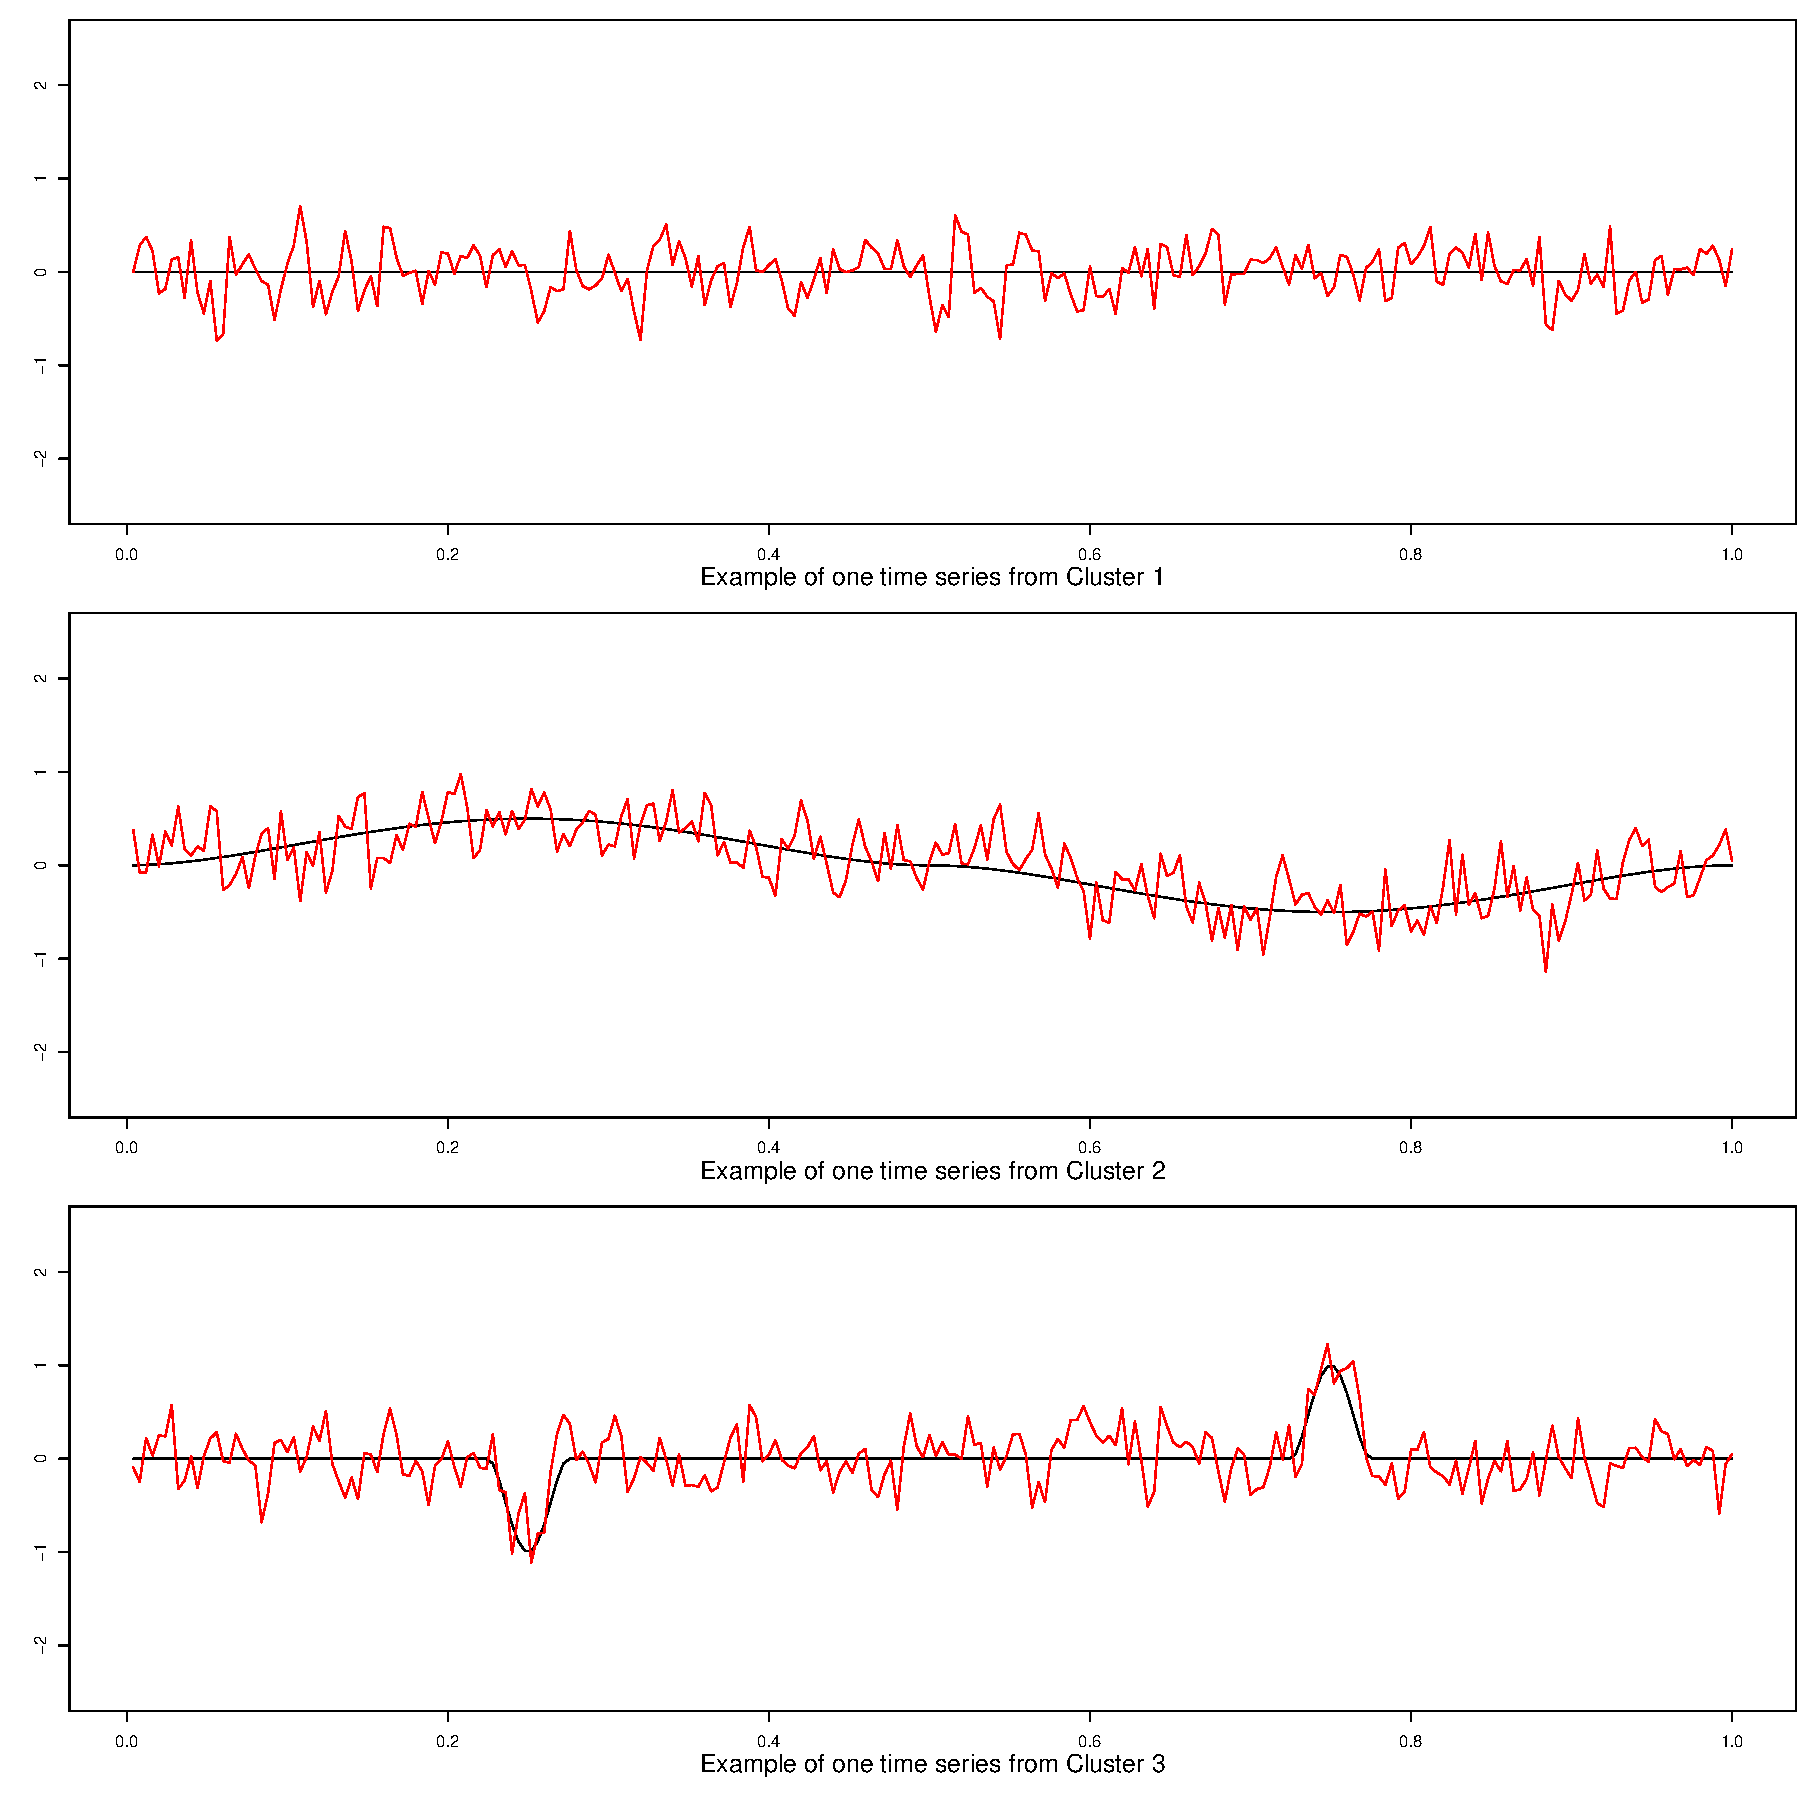
\includegraphics[width=\textwidth]{../output/clustering_functions.pdf}
\caption{In black: the group-specific trend functions $f_1, f_2$ and $f_3$. In red: the time series $\{Y_{it}^\circ : 1 \le t \le T \}$ with $Y_{it}^\circ = f_l(t/T) + \varepsilon_{it}$ for one simulation run and $T=250$.}\label{fig:clustering_fcts}
\end{figure}


The simulation results are reported in Table \ref{tab:clustering}. The entries in Table \ref{tab:clustering}(a) are computed as the number of simulations for which $\widehat{N} = N$ divided by the total number of simulations. They thus specify the empirical probabilities with which the estimate $\widehat{N}$ is equal to the true number of groups $N = 3$. Analogously, the entries of Table \ref{tab:clustering}(b) give the empirical probabilities with which the estimated group structure $\{ \widehat{G}_1,\ldots,\widehat{G}_{\widehat{N}}\}$ equals the true one $\{G_1,G_2,G_3\}$. The results in Table \ref{tab:clustering} nicely illustrate the theoretical properties of our clustering algorithm. According to Proposition \ref{prop:clustering:1}, the probability that $\widehat{N} = N$ and $\{ \widehat{G}_1,\ldots,\widehat{G}_{\widehat{N}}\} = \{G_1,G_2,G_3\}$ should be at least $(1-\alpha)$ asymptotically. For the largest sample size $T = 500$, the empirical probabilities reported in Table \ref{tab:clustering} can indeed be seen to exceed the value $(1-\alpha)$ as predicted by Proposition \ref{prop:clustering:1}. For the smaller sample sizes $T=100$ and $T=250$, in contrast, the empirical probabilities are substantially smaller than $(1-\alpha)$. This reflects the asymptotic nature of Proposition \ref{prop:clustering:1} and is not very surprising. It simply mirrors the fact that for the smaller sample sizes $T=100$ and $T=250$, the effective noise level in the simulated data is quite high.

\begin{table}[t]
\footnotesize{
\begin{center}
\caption{Clustering results for different sample sizes $T$ and nominal sizes $\alpha$.}\label{tab:clustering}
\begin{subtable}[b]{0.48\textwidth}
\centering
\caption{Empirical probabilities that \\ $\widehat{N} = N$}\label{tab:clustering:1}
\renewcommand{\arraystretch}{1.2}
% latex table generated in R 4.3.1 by xtable 1.8-4 package
% 
\begin{tabular}{cccc}
  \hline
  & \multicolumn{3}{c}{nominal size $\alpha$} \\
 $T$ & 0.01 & 0.05 & 0.1 \\
 \hline
100 & 0.000 & 0.002 & 0.005 \\ 
  250 & 0.022 & 0.103 & 0.200 \\ 
  500 & 0.978 & 0.999 & 0.998 \\ 
   \hline
\end{tabular}

\end{subtable}
\begin{subtable}[b]{0.48\textwidth}
\centering
\caption{\centering Empirical probabilities that $\{ \widehat{G}_1,\ldots,\widehat{G}_{\widehat{N}}\} = \{ G_1,G_2,G_3\}$}\label{tab:clustering:2}
\renewcommand{\arraystretch}{1.2}
% latex table generated in R 4.3.1 by xtable 1.8-4 package
% 
\begin{tabular}{cccc}
  \hline
  & \multicolumn{3}{c}{nominal size $\alpha$} \\
 $T$ & 0.01 & 0.05 & 0.1 \\
 \hline
100 & 0.000 & 0.000 & 0.000 \\ 
  250 & 0.021 & 0.098 & 0.187 \\ 
  500 & 0.978 & 0.999 & 0.998 \\ 
   \hline
\end{tabular}

\end{subtable}
\end{center}}
\vspace{-0.5cm}
\end{table}


\begin{figure}[t!]
\centering
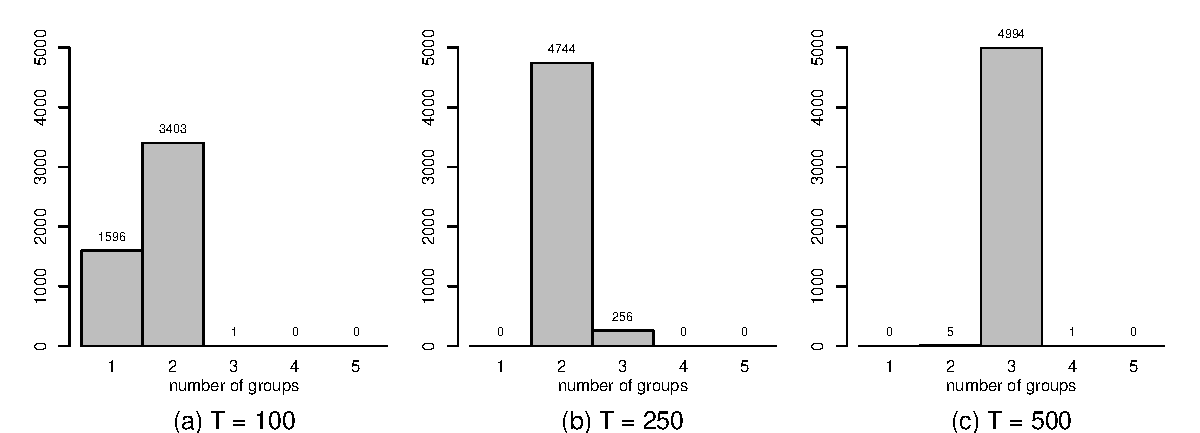
\includegraphics[width=0.95\textwidth]{../output/hist_groups}
\caption{Estimated number of groups $\widehat{N}$ for nominal size $\alpha = 0.05$.
%Each panel corresponds to a different sample size $T$.
}\label{fig:clustering:1}
\vspace{0.25cm}

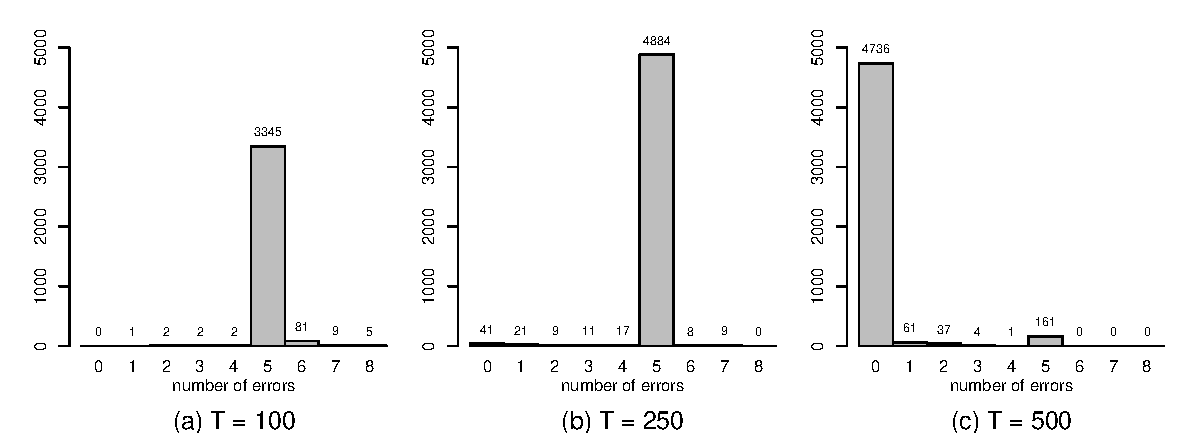
\includegraphics[width=0.95\textwidth]{../output/hist_errors}
\caption{Number of classification errors for nominal size $\alpha = 0.05$.
%Each panel corresponds to a different sample size $T$.
}\label{fig:clustering:2}
\end{figure}

Figures \ref{fig:clustering:1} and \ref{fig:clustering:2} give more insight into what happens for $T=100$ and $T=250$. Figure \ref{fig:clustering:1} shows histograms of the $5000$ simulated values of $\widehat{N}$, while Figure \ref{fig:clustering:2} depicts histograms of the number of classification errors produced by our algorithm. By the number of classification errors, we simply mean the number of incorrectly classified time series, which is formally calculated as 
$\min_{\pi \in S_{\widehat{N}}} \big\{ |G_1 \setminus \widehat{G}_{\pi(1)}| +|G_2 \setminus \widehat{G}_{\pi(2)}| + |G_3 \setminus \widehat{G}_{\pi(3)}| \big\}$
with $S_{\widehat{N}}$ being the set of all permutations of $\{1, 2, \ldots, \widehat{N}\}$. The histogram of Figure \ref{fig:clustering:1} for $T=100$ and $T = 250$ clearly shows that our method underestimates the number of groups. In particular, it fails to detect the difference between two out of three groups in a large number of simulations ($\widehat{N} = 2$ in $3403$ and $4744$ cases out of $5000$ for $T= 100$ and $T=250$, respectively). This is reflected in the corresponding histogram of Figure \ref{fig:clustering:2} which shows that there are exactly $5$ classification errors in $3322$ ($4744$) of the $5000$ simulation runs for $T=100$ ($T=250$). In most of these cases, the estimated group structure $\{ \widehat{G}_1, \widehat{G}_{2}\}$ coincides with either $\{ G_1 \cup G_2,G_3\}$,  $\{ G_1, G_2\cup G_3\}$ or $ \{ G_1 \cup G_3,G_2\}$. In summary, we can conclude that the zero empirical probabilities for $T=100$ and $T=250$ in Table \ref{tab:clustering} are due to the algorithm underestimating the number of groups. Inspecting the histograms for $T=500$, one can see that the performance of the estimators $\widehat{N}$ and $\{ \widehat{G}_1,\ldots, \widehat{G}_{\widehat{N}} \}$ improves significantly. %, even though the corresponding empirical probabilities in Table \ref{tab:clustering} are still somewhat below the target $(1-\alpha)$.


\subsection{Comparison of our clustering algorithm with a benchmark}


We finally compare our clustering algorithm with a simple benchmark. To do so, we consider a simplified version of the simulation setup described in Section \ref{subsec:sim:clustering}. In particular, we use the same setup but without covariates and fixed effects (i.e., $\boldsymbol{\beta}_i = 0$ and $\alpha_i = 0$ for all $i$). The benchmark method proceeds as follows: 
\begin{enumerate}[label=\textit{Step \arabic*}.,leftmargin=1.5cm,itemsep=0pt,parsep=0pt,topsep=3pt]
\item For each $i$, estimate the trend function $m_i$ by a standard local linear estimator $\widehat{m}_i = \widehat{m}_{i,h}$ with bandwidth $h$.
  %We consider two choices for the bandwidth: $h_1 = \min \{h\in H_t\}$ and $h_2 = \max\{h \in H_T\}$. As we will see further, the choice of bandwidth significantly affects the results.
\item Estimate the distance between $\widehat{m}_i$ and $\widehat{m}_j$ by taking the supremum metric 
\[ d_{ij}^{\textnormal{bmk}} = \sup_{u \in [0,1]} |\widehat{m}_i(u) - \widehat{m}_j(u)|. \]
%  Compute a simple $\mathcal{L}_2$ distance measure $d_{ij}$ between $\widehat{m}_i$ and $\widehat{m}_j$, e.g.
%\[ d_{ij} = \int_0^1 (\widehat{m}_i(w) - \widehat{m}_j(w))^2 dw. \]
\item Construct the following dissimilarity measure from these supremum distances:
\[ \widehat{\Delta}^{\textnormal{bmk}}(S,S') = \max_{i \in S,j \in S'} d_{ij}^{\textnormal{bmk}}. \]
\item Run a HAC algorithm with the computed dissimilarities. 
\end{enumerate}
Our multiscale approach can be regarded as a refinement of this very natural and intuitive approach: it replaces the simple bandwidth-dependent distance measure $d_{ij}^{\textnormal{bmk}}$ by the multiscale distance measure $d_{ij} = \max_{(u, h) \in \mathcal{G}_T}\hat{\psi}^0_{ij, T}(u, h)$ and provides a way to estimate the number of clusters $N$. As the benchmark algorithm does not come with an estimate of the number of clusters $N$, we assume $N=3$ to be known in what follows. 

%This procedure serves as a straightforward and intuitive benchmark, with our approach being a refinement of it. In particular, our approach replaces the simple distance measure $d_{ij}$ by a more advanced multiscale distance measure and provides a way to estimate the number of clusters -- a feature not included in the benchmark procedure. For the sake of fair comparison, we assume that the number of clusters $N=3$ is known, and thus, do not provide an estimate of the number of groups $\widehat{N}$.


We implement our clustering algorithm in exactly the same way as in Section \ref{subsec:sim:clustering}. To run the benchmark algorithm in practice, we need to discretize the supremum over all time points $u \in [0,1]$ in Step 2 of the algorithm. To make the comparison as fair as possible, we replace this supremum by the maximum over all points $u \in U_T$, where $U_T$ is the grid of locations defined in \eqref{eq:grid-loc} that underlies the location-scale grid $\mathcal{G}_T = U_T \times H_T$ of our multiscale test. Moreover, we need to choose a bandwidth to run the benchmark algorithm. We consider six different choices: $h_k = h_{\min} + c_k (h_{\max} - h_{\min})$ with $c_k = 0.2(k-1)$ for $k=1,\ldots,6$.

%We implement the clustering algorithm as in Section \ref{subsec:sim:clustering} with one small difference. Computational time of the benchmark procedure exceeds significantly the computational time needed for our method (presumably, due to the lack of the discretization of the grid), hence, in order to lighten the computational burden, instead of $5000$ samples, we simulate $1000$ samples for this simulation exercise.


\begin{table}[t!]
\centering
\caption{Empirical probabilities that $\{ \widehat{G}_1,\ldots,\widehat{G}_{\widehat{N}}\} = \{ G_1,G_2,G_3\}$ for the proposed clustering approach with an estimated long-run variance ($\mathcal{T}_{\text{MS}}$) and with the true theoretical value of the long-run variance ($\mathcal{T}_{\text{MS, true lrv}}$) and the benchmark procedures $\mathcal{T}_{\text{bmk, }1} - \mathcal{T}_{\text{bmk, }6}$ corresponding to bandwidths $h_1 - h_6$ for different sample sizes $T$.}\label{tab:clustering:comparison}
\newcolumntype{Z}{>{\centering\arraybackslash}X}
{\color{red}% latex table generated in R 4.3.1 by xtable 1.8-4 package
% 
\begin{tabular}{ccccccccc}
  \hline
  & $\mathcal{T}_{\text{MS}}$ & $\mathcal{T}_{\text{MS, true lrv}}$ & $\mathcal{T}_{\text{bmk, }1}$ & $\mathcal{T}_{\text{bmk, }2}$ & $\mathcal{T}_{\text{bmk, }3}$ & $\mathcal{T}_{\text{bmk, }4}$ & $\mathcal{T}_{\text{bmk, }5}$ & $\mathcal{T}_{\text{bmk, }6}$\\
 \hline
$T = 100$ & 0.227 & 0.248 & 0.016 & 0.003 & 0.001 & 0.001 & 0.002 & 0.002 \\ 
  $T = 250$ & 0.935 & 0.951 & 0.188 & 0.066 & 0.014 & 0.007 & 0.001 & 0.003 \\ 
  $T = 500$ & 1.000 & 1.000 & 0.341 & 0.406 & 0.143 & 0.057 & 0.022 & 0.020 \\ 
   \hline
\end{tabular}
%This simulation was done for the following values of the parameters: n_ts = 15, with 1000 simulations for calculating size and power. Furthermore, for the error process we have a = 0.25 and sigma = 0.25. There are no fixed effects. The grid is standard.
}
%{\color{red}
%\begin{tabular}{ccccccccc}
%  \hline
%  & $\mathcal{T}_{\text{MS}}$ & $\mathcal{T}_{\text{MS, true lrv}}$ & $\mathcal{T}_{\text{bm, }1}$ & $\mathcal{T}_{\text{bm, }2}$ & $\mathcal{T}_{\text{bm, }3}$ & $\mathcal{T}_{\text{bm, }4}$ & $\mathcal{T}_{\text{bm, }5}$ & $\mathcal{T}_{\text{bm, }6}$ \\
% \hline
%$T= 100$ & 0.007 & 0.029 & 0.066& 0.066 & 0 & 0  & 0 & 0\\ 
%$T=  250$ & 0.742 & 0.903 & 0.943 & 0.066 & 0 & 0 & 0 & 0\\ 
%$T=  500$ & 1.000 & 1.000 & 1.000 & 0.066& 0 & 0 & 0 & 0\\ 
%   \hline
%\end{tabular}}
\end{table}

%\addtocounter{table}{-1} 
%\begin{table}[t]
%\footnotesize{
%\begin{center}
%\caption{Clustering results for different sample sizes $T$ and nominal sizes $\alpha$.}\label{tab:clustering}
%\begin{subtable}[b]{0.48\textwidth}
%\centering
%\caption{Empirical probabilities that \\ $\widehat{N} = N$}\label{tab:clustering:1}
%\renewcommand{\arraystretch}{1.2}
%% latex table generated in R 4.3.1 by xtable 1.8-4 package
% 
\begin{tabular}{cccc}
  \hline
  & \multicolumn{3}{c}{nominal size $\alpha$} \\
 $T$ & 0.01 & 0.05 & 0.1 \\
 \hline
100 & 0.000 & 0.002 & 0.005 \\ 
  250 & 0.022 & 0.103 & 0.200 \\ 
  500 & 0.978 & 0.999 & 0.998 \\ 
   \hline
\end{tabular}

%\end{subtable}
%\begin{subtable}[b]{0.48\textwidth}
%\centering
%\caption{\centering Empirical probabilities that $\{ \widehat{G}_1,\ldots,\widehat{G}_{\widehat{N}}\} = \{ G_1,G_2,G_3\}$}\label{tab:clustering:2}
%\renewcommand{\arraystretch}{1.2}
%% latex table generated in R 4.3.1 by xtable 1.8-4 package
% 
\begin{tabular}{cccc}
  \hline
  & \multicolumn{3}{c}{nominal size $\alpha$} \\
 $T$ & 0.01 & 0.05 & 0.1 \\
 \hline
100 & 0.000 & 0.000 & 0.000 \\ 
  250 & 0.021 & 0.098 & 0.187 \\ 
  500 & 0.978 & 0.999 & 0.998 \\ 
   \hline
\end{tabular}

%\end{subtable}
%\end{center}}
%\vspace{-0.5cm}
%\end{table}
%
%
%\begin{figure}[t!]
%\centering
%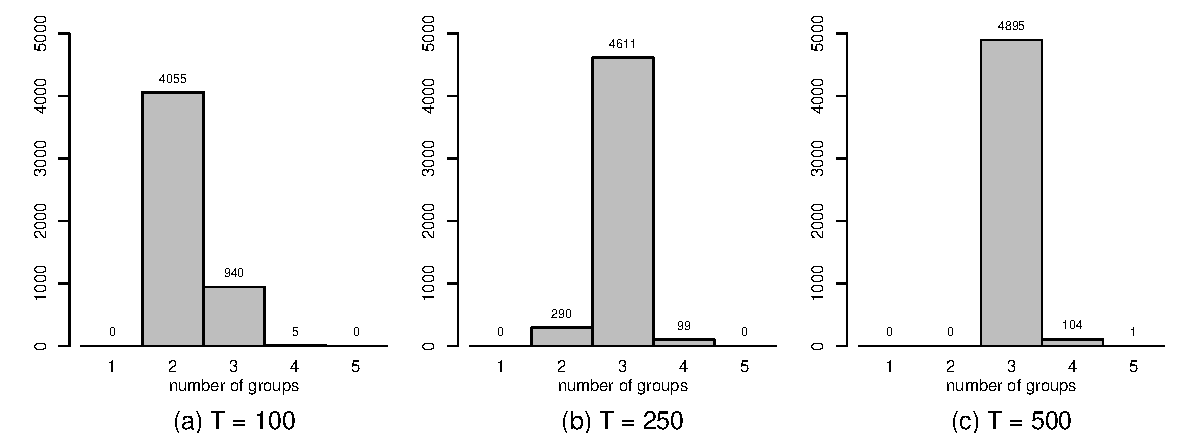
\includegraphics[width=0.95\textwidth]{output/plots/sim/histograms_groups}
%\caption{Estimated number of groups $\widehat{N}$ for nominal size $\alpha = 0.05$. 
%%Each panel corresponds to a different sample size $T$.
%}\label{fig:clustering:1}
%\vspace{0.25cm}
%
%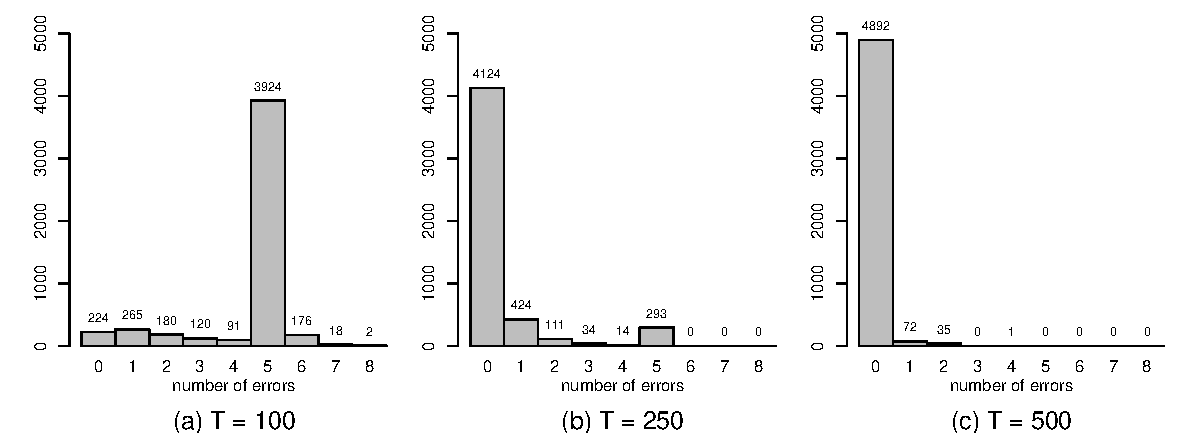
\includegraphics[width=0.95\textwidth]{output/plots/sim/histograms_errors}
%\caption{Number of classification errors for nominal size $\alpha = 0.05$. 
%%Each panel corresponds to a different sample size $T$.
%}\label{fig:clustering:2}
%\end{figure}


The simulation results are reported in Table \ref{tab:clustering:comparison}. The entries of the table give the empirical probabilities with which the estimated group structure $\{ \widehat{G}_1,\ldots,\widehat{G}_3\}$ equals the true one $\{G_1,G_2,G_3\}$.
\textcolor{blue}{[Ideally, would like to have the following results:]
The two main take-away messages are these:
(i) The performance of the benchmark procedure is heavily influenced by the choice of bandwidth.
(ii) The performance of our multiscale method is comparable to that of the benchmark with the best choice of bandwidth.
This can be interpreted as follows: our multiscale method automatically selects the ``right'' scale(s) or bandwidth(s), i.e., those which are most suitable for comparing the trend curves. }


%{\color{red} The results highlight a significant distinction: the benchmark procedure's outcomes are heavily influenced by the selection of bandwidth, a limitation not observed in our clustering approach. Furthermore, with large sample sizes, the empirical probabilities of success using our clustering approach—even with an estimated number of clusters—are quite high. In contrast, the benchmark procedure lacks a method for estimating the number of clusters. 
%Most importantly, it demonstrates that our method provides robust results whereas the benchmark depends very strongly on the choice of bandwidth.
%}


%\subsection*{Simulation results}
%
%As a robustness check, we calculate the actual size values within a slightly simplified simulation context. Specifically, we do not include any covariates in the model but only the fixed effects $\alpha_i$ with $\rho = 0.1$. Additionally, we explore larger sample sizes ($T=100, 250, 500, 750, 1000$), albeit with a sparser grid $\mathcal{G}_T$ for computational efficiency: we define the grid as $\mathcal{G}_T = U_T \times H_T$, where $U_T = \big\{ u \in [0,1]: u = \textstyle{\frac{10t}{T}} \text{ for some } t \in \mathbb{N} \big\}$ and $H_T = \big\{ h \in \big[ \textstyle{\frac{\log T}{T}}, \textstyle{\frac{1}{4}} \big]:  h = \textstyle{\frac{10t - 3}{T}} \text{ for some } t \in \mathbb{N} \big\}$. The findings are reported in Table \ref{tab:size:no_covariates}. Notably, the results exhibit minimal deviation from the primary simulation scenarios. One thing that is potentially worth mentioning is that we can see a discernible ``bump'' in the actual size values for moderate sample sizes ($T = 250, 500$). This phenomenon persists across various specifications tested, including scenarios with $\rho = 0$ which indicates no dependence between the time series. This specific pattern can be explained by the trade-off between the sample size and the dimensionality of the problem, i.e., the number of tests we carry out simultaneously. For moderate value of the sample sizes ($T =250, 500$) the number of comparisons is already quite large ($15750$ and $63000$ simultaneous comparisons, respectively), while the effective sample size for testing individual null hypothesis remains relatively modest. However, empirical evidence suggests that the size values stabilize for larger sample sizes ($T = 750, 1000$) suggesting robust test performance even in the face of significant high dimensionality of the problem ($149625 $ and $262500$ simultaneous comparisons, respectively).
%\addtocounter{table}{-1} 
%\begin{table}[t]
%\footnotesize{
%\begin{center}
%\caption{Size of the multiscale test for the case without any covariates and $\rho = 0.1$ for different sample sizes $T$ and nominal sizes $\alpha$.}
%\label{tab:size:no_covariates}
%\renewcommand{\arraystretch}{1.2}
%% latex table generated in R 4.3.1 by xtable 1.8-4 package
% 
\begin{tabular}{cccc}
  \hline
  & \multicolumn{3}{c}{nominal size $\alpha$} \\
 $T$ & 0.01 & 0.05 & 0.1 \\
 \hline
100 & 0.007 & 0.030 & 0.069 \\ 
  250 & 0.019 & 0.078 & 0.140 \\ 
  500 & 0.016 & 0.063 & 0.128 \\ 
  750 & 0.011 & 0.062 & 0.118 \\ 
  1000 & 0.011 & 0.054 & 0.114 \\ 
   \hline
\end{tabular}
%This simulation was done for the seed 113355, for the following values of the parameters: n_ts = 15, with 5000 simulations for calculating size and power and 5000 simulations to calculate the Gaussian quantiles. Furthermore, for the error process we have a = 0.25 and sigma = 0.25. We do not have any covarites. For the fixed effect, we have rho = 0.1. The grid is fine (growing with the sample size)

%\end{center}}
%\vspace{-0.4cm}
%\end{table}
  



\section{Application to GDP growth data}\label{sec:app:gdp}


In what follows, we revisit an application example from \cite{Zhang2012}. The aim is to test the hypothesis of a common trend in the GDP growth time series of several OECD countries. Since we do not have access to the original dataset of \cite{Zhang2012} and we do not know the exact data specifications used there, we work with data from the following common sources: Refinitiv Datastream, the OECD.Stat database, Federal Reserve Economics Data (FRED) and the Barro-Lee Educational Attainment dataset \citep*{Barro2013}. We consider a data specification that is as close as possible to the one in \cite{Zhang2012} with one important distinction: In the original study, the authors examined $16$ OECD countries (not specifying which ones) over the time period from the fourth quarter of 1975 up to and including the third quarter of 2010, whereas we consider only $11$ countries (Australia, Austria, Canada, Finland, France, Germany, Japan, Norway, Switzerland, UK and USA) over the same time span. The reason is that we have access to data of good quality only for these 11 countries. 
%In particular, the OECD.Stat database, which is our main source for data on major economic indicators, contains quarterly data of good quality only for the above mentioned $11$ countries. 
In the following list, we specify the data for our analysis.\footnote{All data were accessed and downloaded on 7 December 2021.}

\begin{itemize}[leftmargin=0.5cm]
\item \textbf{Gross domestic product ($\boldsymbol{GDP}$):} We use freely available data on \textit{Gross Domestic Product -- Expenditure Approach} from the OECD.Stat %\nocite{OECD} 
database (\texttt{https://stats.\linebreak oecd.org/Index.aspx}). To be as close as possible to the specification of the data in \cite{Zhang2012}, we use seasonally adjusted quarterly data on GDP expressed in millions of 2015 US dollars.\footnote{Since the publication of \cite{Zhang2012}, the OECD reference year has changed from 2005 to 2015. We have decided to analyse the latest version of the data in order to be able to make more accurate and up-to-date conclusions.} 
%The data are available from 1960 to 2021 which fully covers the time period that we take into consideration. 

\item \textbf{Capital ($\boldsymbol{K}$):} We use data on \textit{Gross Fixed Capital Formation} from the OECD.Stat %\nocite{OECD} 
database. The data are at a quarterly frequency, seasonally adjusted, and expressed in millions of $2015$ US dollars. In contrast to \cite{Zhang2012}, who use data on \textit{Capital Stock at Constant National Prices}, we choose to work with gross fixed capital formation due to data availability. It is worth noting that since accurate data on capital stock is notoriously difficult to collect, the use of gross fixed capital formation as a measure of capital is standard in the literature; see e.g.\ \cite{Sharma1994}, \cite{Lee2002} and \cite{Lee2005}.
%We repeat the analysis using the quarterly data on Gross Fixed Capital Formation instead of Capital Stock in the Appendix.

\item \textbf{Labour ($\boldsymbol{L}$):} We collect data on the \textit{Number of Employed People} from various sources. For most of the countries (Austria, Australia, Canada, Germany, Japan, UK and USA), we download the OECD data on \textit{Employed Population: Aged 15 and Over} retrieved from FRED (\texttt{https://fred.stlouisfed.org/}). %\nocite{OECDempl} 
The data for France and Switzerland were downloaded from Refinitiv Datastream. For all of the aforementioned countries, the observations are at a quarterly frequency and seasonally adjusted. The data for Finland and Norway were also obtained via Refinitiv Datastream, however, the only quarterly time series that are long enough for our purposes are not seasonally adjusted. Hence, for these two countries, we perform the seasonal adjustment ourselves. We in particular use the default method of the function \verb|seas| from the \verb|R| package \verb|seasonal| \citep*{Sax2018} which is an interface to X-13-ARIMA-SEATS, the seasonal adjustment software used by the US Census Bureau. 
%We repeat the analysis using not seasonally adjusted data for all of the $11$ countries as a robustness check and we report the results in the Appendix.
For all of the countries, the data are given in thousands of persons.

\item \textbf{Human capital ($\boldsymbol{H}$):} We use \textit{Educational Attainment for Population Aged 25 and Over} collected from \texttt{http://www.barrolee.com} as a measure of human capital. Since the only available data is five-year census data, we follow \cite{Zhang2012} and use linear interpolation between the observations and constant extrapolation on the boundaries (second and third quarters of 2010) to obtain the quarterly time series.
\end{itemize}


For each of the $n=11$ countries in our sample, we thus observe a quarterly time series $\mathcal{T}_i = \{(Y_{it}, \X_{it}): 1 \le t \le T \}$ of length $T = 140$, where $Y_{it} = \Delta \ln GDP_{it} := \ln GDP_{it} - \ln GDP_{i(t-1)}$ and $\X_{it} = (\Delta \ln L_{it}, \Delta \ln K_{it}, \Delta \ln H_{it})^\top$ with $\Delta \ln L_{it} := \ln L_{it} - \ln L_{i(t-1)}$, $\Delta \ln K_{it} := \ln K_{it} - \ln K_{i(t-1)}$ and $\Delta \ln H_{it} := \ln H_{it} - \ln H_{i(t-1)}$. Without loss of generality, we let $\Delta \ln GDP_{i1} = \Delta \ln L_{i1} = \Delta \ln K_{i1} = \Delta \ln H_{i1} = 0$. Each time series $\mathcal{T}_i$ is assumed to follow the model $Y_{it} = m_i(t/T) + \bfbeta^\top_i \X_{it} + \alpha_i + \varepsilon_{it}$, or equivalently,  
\begin{align}
\Delta \ln GDP_{it}
 & = m_i \Big( \frac{t}{T} \Big) + \beta_{i, 1} \Delta \ln L_{it} + \beta_{i, 2} \Delta \ln K_{it} + \beta_{i, 3} \Delta \ln H_{it} + \alpha_i + \varepsilon_{it} \label{eq:model:app}
\end{align}
for $1 \le t \le T$, where $\bfbeta_i = (\beta_{i, 1}, \beta_{i, 2}, \beta_{i, 3})^\top$ is a vector of unknown parameters, $m_i$ is a country-specific unknown nonparametric time trend and $\alpha_i$ is a country-specific fixed effect. 


In order to test the null hypothesis $H_0: m_1 = \ldots = m_n$ with $n = 11$ in model \eqref{eq:model:app}, we implement our multiscale test as follows: 
\begin{itemize}[leftmargin=0.5cm]

\item We choose $K$ to be the Epanechnikov kernel and consider the set of location-scale points $\mathcal{G}_T = U_T \times H_T$, where 
%\begin{align*}
$U_T = \big\{ u \in [0,1]: u = \textstyle{\frac{8t + 1}{2T}} \text{ for some } t \in \naturals \big\}$ and
$H_T = \big\{ h \in \big[ \textstyle{\frac{\log T}{T}}, \textstyle{\frac{1}{4}} \big]:  h = \textstyle{\frac{4t}{T}} \text{ for some } t \in \naturals \big\}$. 
%\end{align*}
We thus take into account all locations $u$ on an equidistant grid $U_T$ with step length $4/T$ and all scales $h=4/T, 8/T, 12/T,\ldots$ with $\log T /T \le h \le 1/4$. 
%Note that $\mathcal{G}_T$ is not a subset of $\mathcal{G}_T^{\text{full}}$ since we do not assume that the considered locations take the form of $u = t/T$ for some $1 \leq t \leq T$. It can be shown that with this choice of the grid the theoretical properties of our method remain the same. 
The choice of the grid $\grid$ is motivated by the quarterly frequency of the data: each interval $\interval$ with $(u,h) \in \mathcal{G}_T$ spans $8, 16, 24, \ldots$ quarters, i.e., $2, 4, 6, \ldots$ years. The lower bound $\log T / T$ on the scales $h$ in $H_T$ is motivated by Assumption \ref{C-h}, which requires that $\log T /T \ll h_{\min}$ (given that all moments of $\varepsilon_{it}$ exist).

%\item The estimators $\widehat{\bfbeta}_i$ and $\widehat{\alpha}_i$ of the unknown parameters $\bfbeta_i$ and the fixed effects $\alpha_i$ are computed as described in Section ??. 
 
\item To obtain an estimator $\widehat{\sigma}_i^2$ of the long-run error variance $\sigma^2_i$ for each $i$, we assume that the error process $\mathcal{E}_i$ follows an AR($p_i$) model and apply the difference-based procedure of \cite{KhismatullinaVogt2020} to the augmented time series $\{\widehat{Y}_{it}: 1\leq t \leq T\}$ with $\widehat{Y}_{it} = Y_{it} - \widehat{\bfbeta}_i^\top \X_{it} - \widehat{\alpha}_{i}$. We set the tuning parameters $q$ and $r$ of the procedure to $20$ and $10$, respectively, and choose the AR order $p_i$ by minimizing BIC, which yields $p_i = 3$ for Australia, Canada and the UK and $p_i = 1$ for all other countries.\footnote{We also calculated the values of other information criteria such as FPE, AIC and HQ which, in most of the cases, resulted in the same values of $p_i$.} 

\item The critical values $q_{n, T}(\alpha)$ are computed by Monte Carlo methods as described in Section \ref{subsec:test:impl}, where we set $L=5000$.
\end{itemize}
Besides these choices, we construct and implement the multiscale test exactly as described in Section \ref{sec:test}.  


The thus implemented multiscale test rejects the global null hypothesis $H_0$ at the usual significance levels $\alpha =0.01,0.05, 0.1$. This result is in line with the findings in \cite{Zhang2012} where the null hypothesis of a common trend is rejected at level $\alpha = 0.1$.
%\footnote{Other significance levels were not considered. \textcolor{blue}{[Not really, they report the p-values for testing the null using various bandwidths; in the text they only mention rejection at level 0.1, but I guess it is because that some (not all) p-values for their test are above 0.05.]}} 
The main advantage of our multiscale test over the method in \cite{Zhang2012} is that it is much more informative. In particular, it provides information about \textit{which} of the $n=11$ countries have different trends and \textit{where} the trends differ. This information is presented graphically in Figures~\ref{fig:Australia:Norway}--\ref{fig:Australia:France}. Each figure corresponds to a specific pair of countries $(i, j)$ and is divided into three panels (a)--(c). 
Panel (a) shows the augmented time series $\{\widehat{Y}_{it}: 1 \le t \le T\}$ and $\{\widehat{Y}_{jt}: 1 \le t \le T\}$ for the two countries $i$ and $j$ that are compared. 
Panel (b) presents smoothed versions of the time series from (a), in particular, it shows local linear kernel estimates of the two trend functions $m_i$ and $m_j$, where the bandwidth is set to $14$ quarters (that is, to $0.1$ in terms of rescaled time) and an Epanechnikov kernel is used. Panel (c) presents the results produced by our test for the significance level $\alpha = 0.05$:
%\footnote{The results for $\alpha = 0.1$ are very similar and thus omitted.}: 
it depicts in grey the set $\mathcal{S}^{[i, j]}(\alpha)$ of all the intervals for which the test rejects the local null $H_0^{[i, j]}(u, h)$. The set of minimal intervals $\mathcal{S}^{[i, j]}_{min}(\alpha) \subseteq \mathcal{S}^{[i, j]}(\alpha)$ is highlighted in black. According to \eqref{eq:CS-v2}, we can make the following simultaneous confidence statement about the intervals plotted in panels (c) of Figures \ref{fig:Australia:Norway}--\ref{fig:Australia:France}: we can claim, with confidence of about $95\%$, that there is a difference between the functions $m_i$ and $m_j$ on each of these intervals. 


\begin{sidewaysfigure}[p!]
\begin{minipage}[t]{0.24\textwidth}
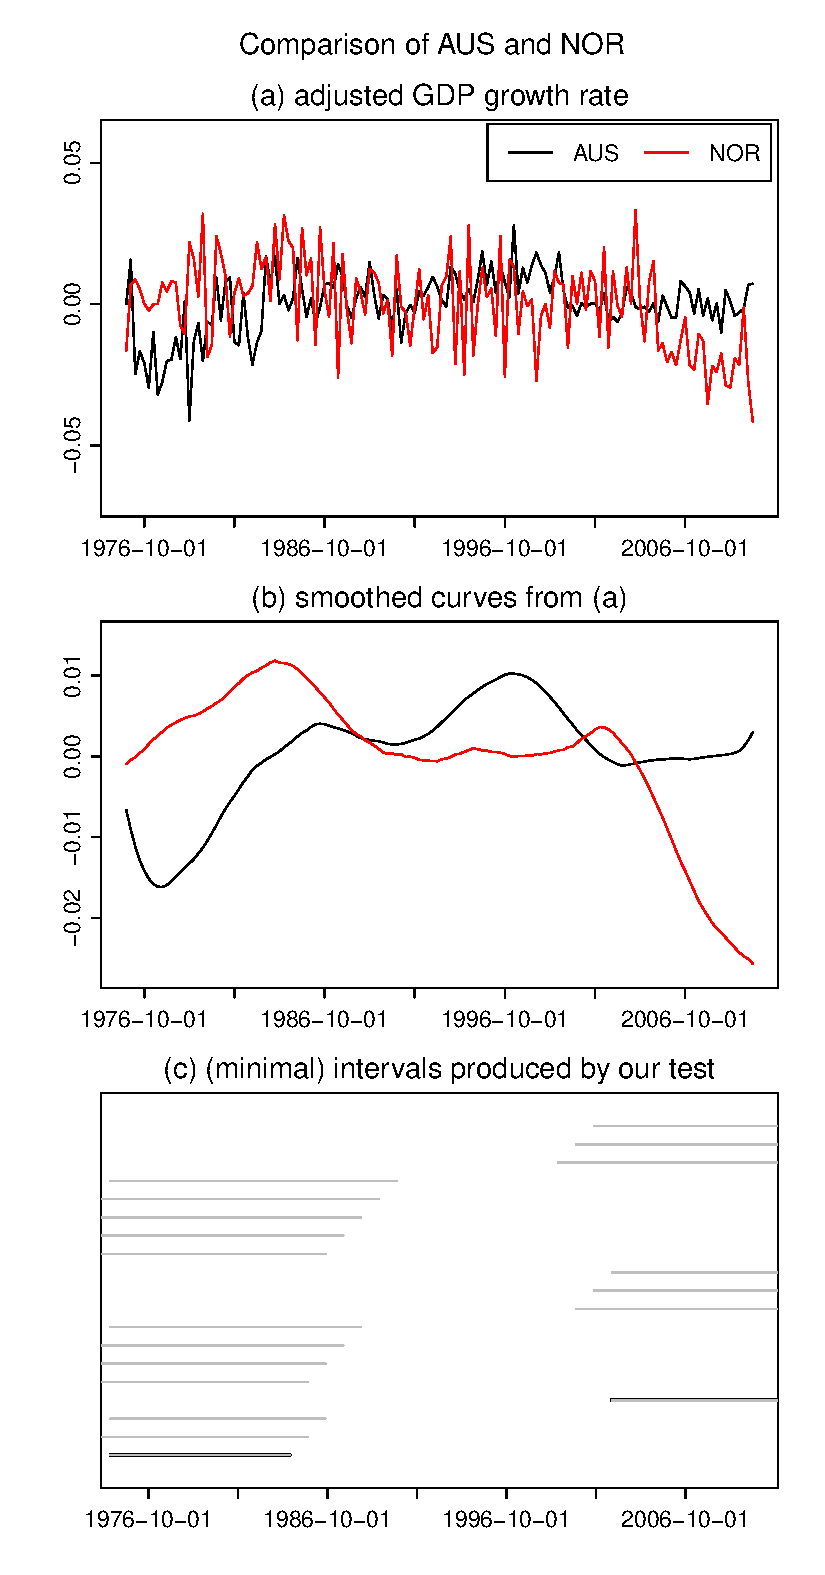
\includegraphics[width=\textwidth]{output/plots/gdp/AUS_vs_NOR}
\caption{Test results for the comparison of Australia and Norway.}\label{fig:Australia:Norway}
\end{minipage}
\hspace{0.1cm}
\begin{minipage}[t]{0.24\textwidth}
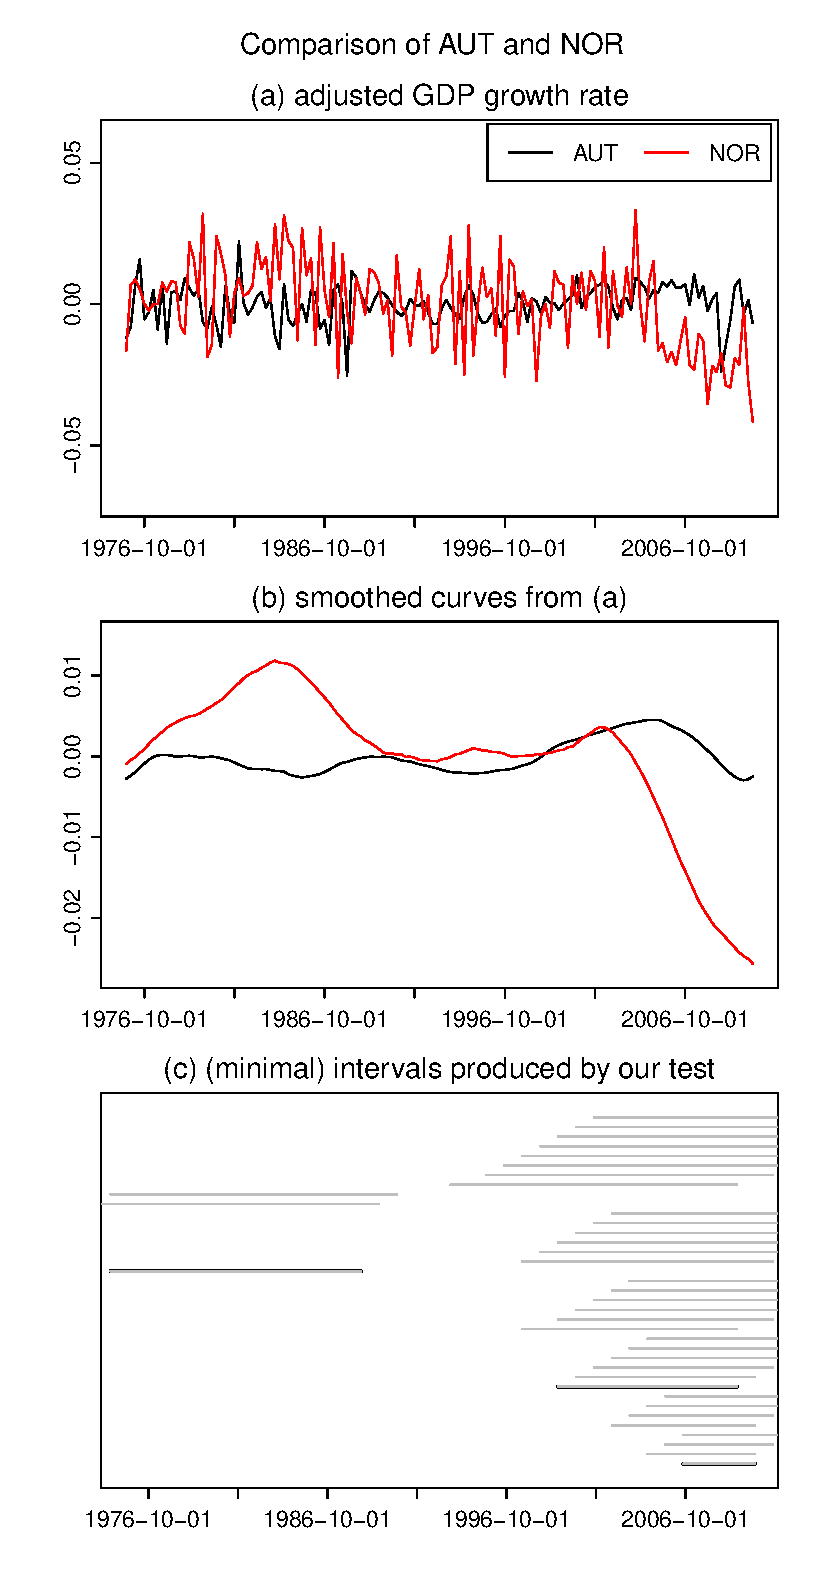
\includegraphics[width=\textwidth]{output/plots/gdp/AUT_vs_NOR}
\caption{Test results for the comparison of Austria and Norway.}\label{fig:Austria:Norway}
\end{minipage}
\hspace{0.1cm}
\begin{minipage}[t]{0.24\textwidth}
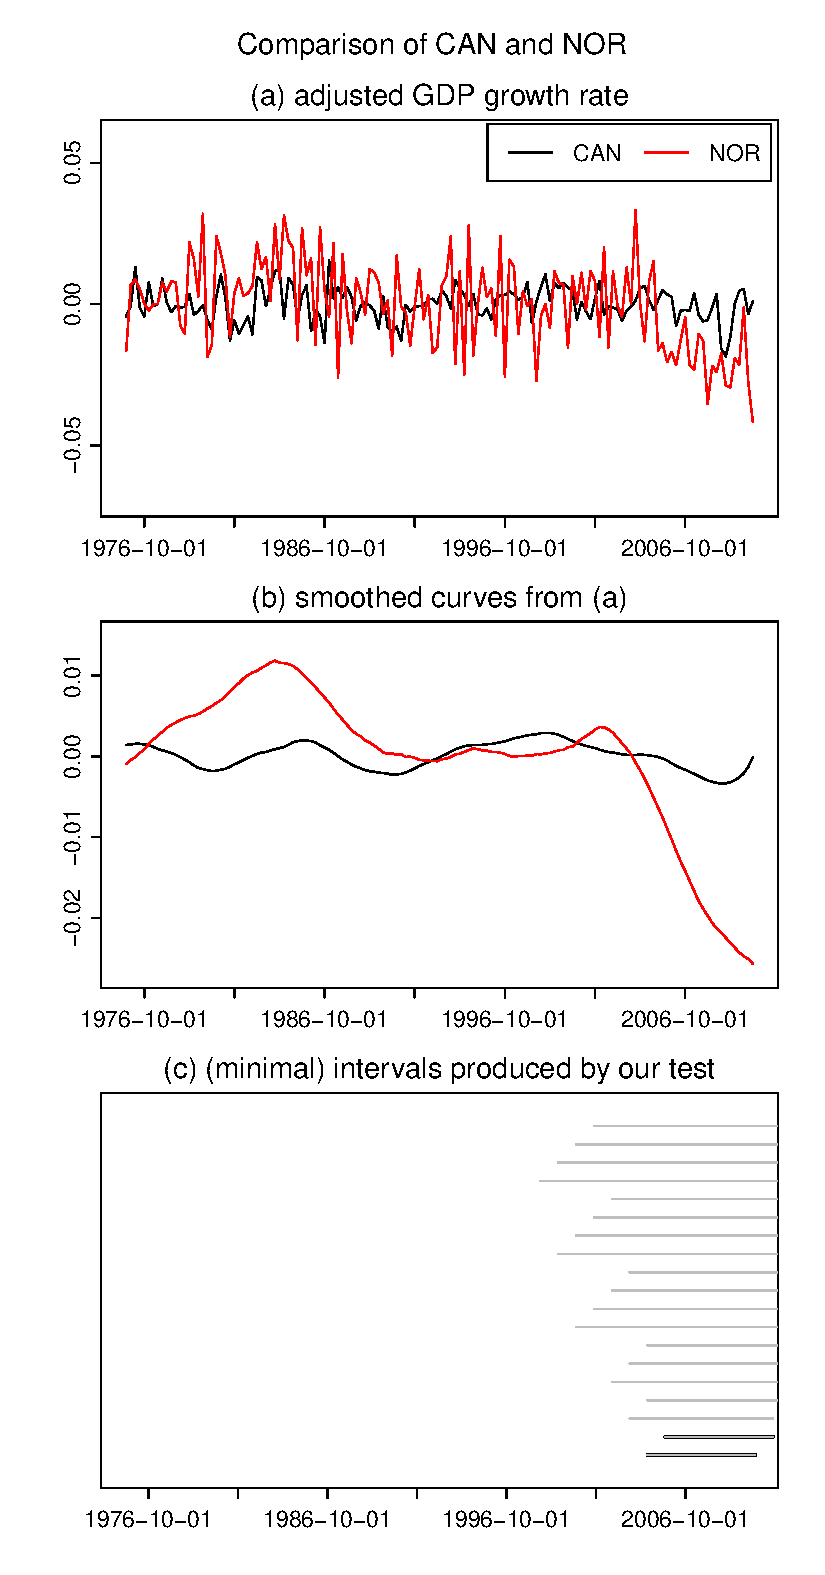
\includegraphics[width=\textwidth]{output/plots/gdp/CAN_vs_NOR}
\caption{Test results for the comparison of Canada and Norway.}\label{fig:Canada:Norway}
\end{minipage}
\hspace{0.1cm}
\begin{minipage}[t]{0.24\textwidth}
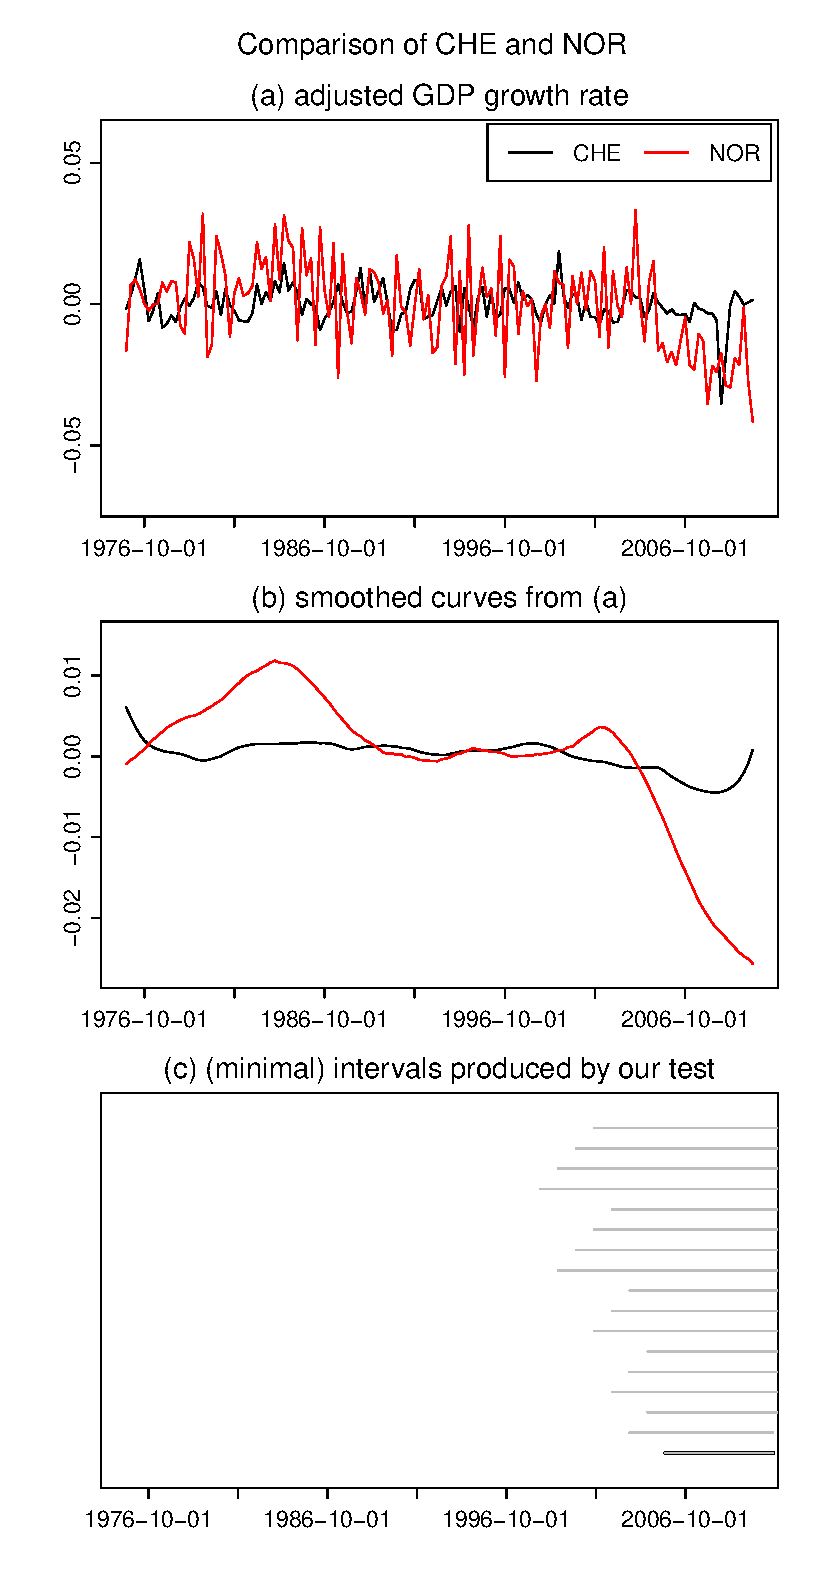
\includegraphics[width=\textwidth]{output/plots/gdp/CHE_vs_NOR}
\caption{Test results for the comparison of Switzerland and Norway.}\label{fig:Switzerland:Norway}
\end{minipage}
\caption*{Note: In each figure, panel (a) shows the two augmented time series, panel (b) presents smoothed versions of the augmented time series, and panel (c) depicts the set of intervals $\mathcal{S}^{[i, j]}(\alpha)$ in grey and the subset of minimal intervals $\mathcal{S}^{[i, j]}_{min}(\alpha)$ in black. }
\end{sidewaysfigure}


\begin{sidewaysfigure}[p!]
\begin{minipage}[t]{0.24\textwidth}
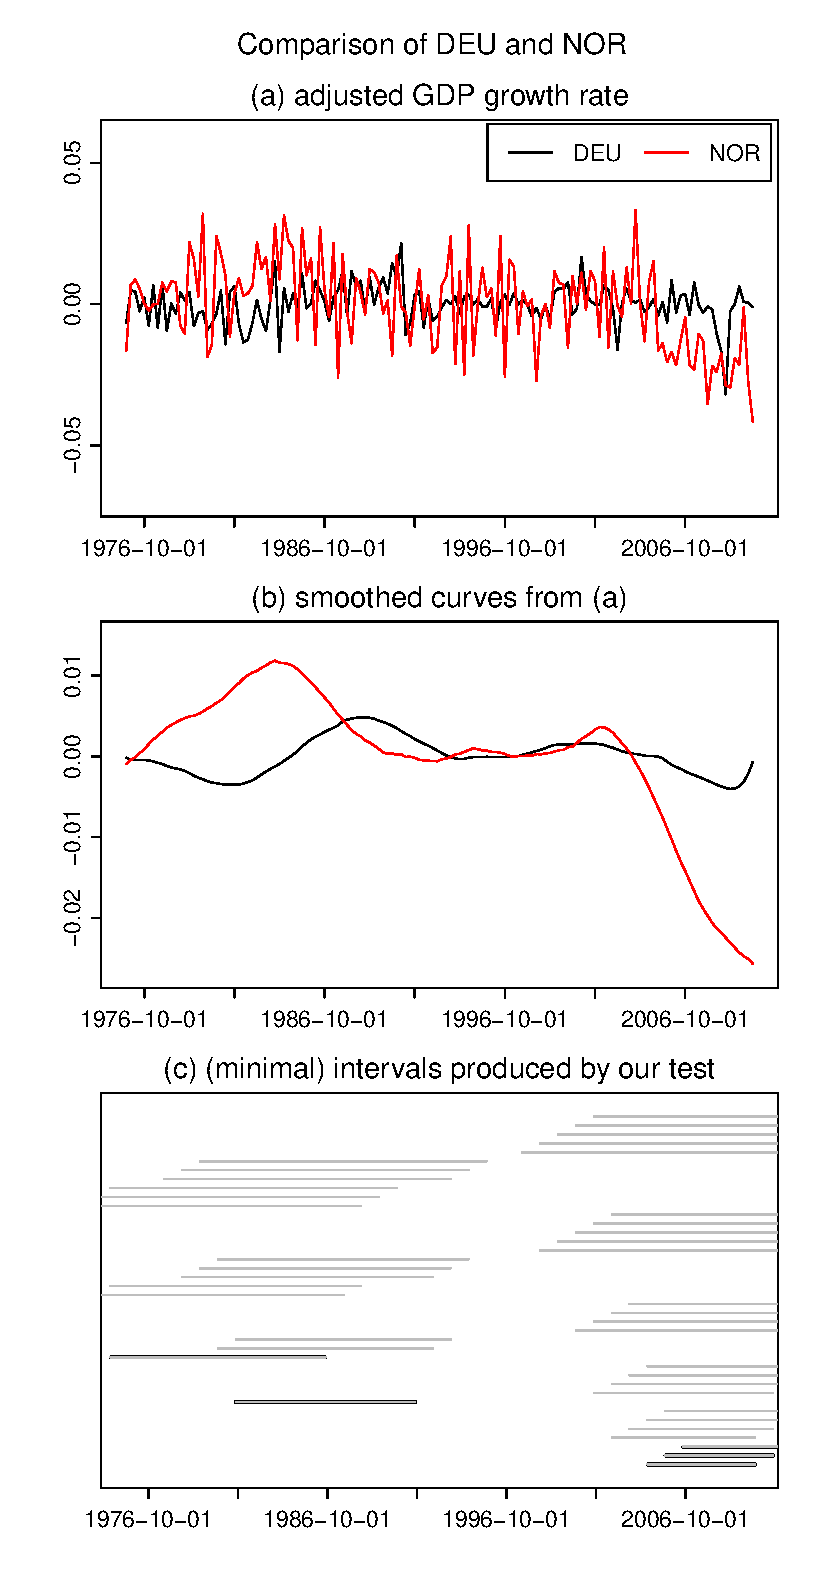
\includegraphics[width=\textwidth]{output/plots/gdp/DEU_vs_NOR}
\caption{Test results for the comparison of Germany and Norway.}\label{fig:Germany:Norway}
\end{minipage}
\hspace{0.1cm}
\begin{minipage}[t]{0.24\textwidth}
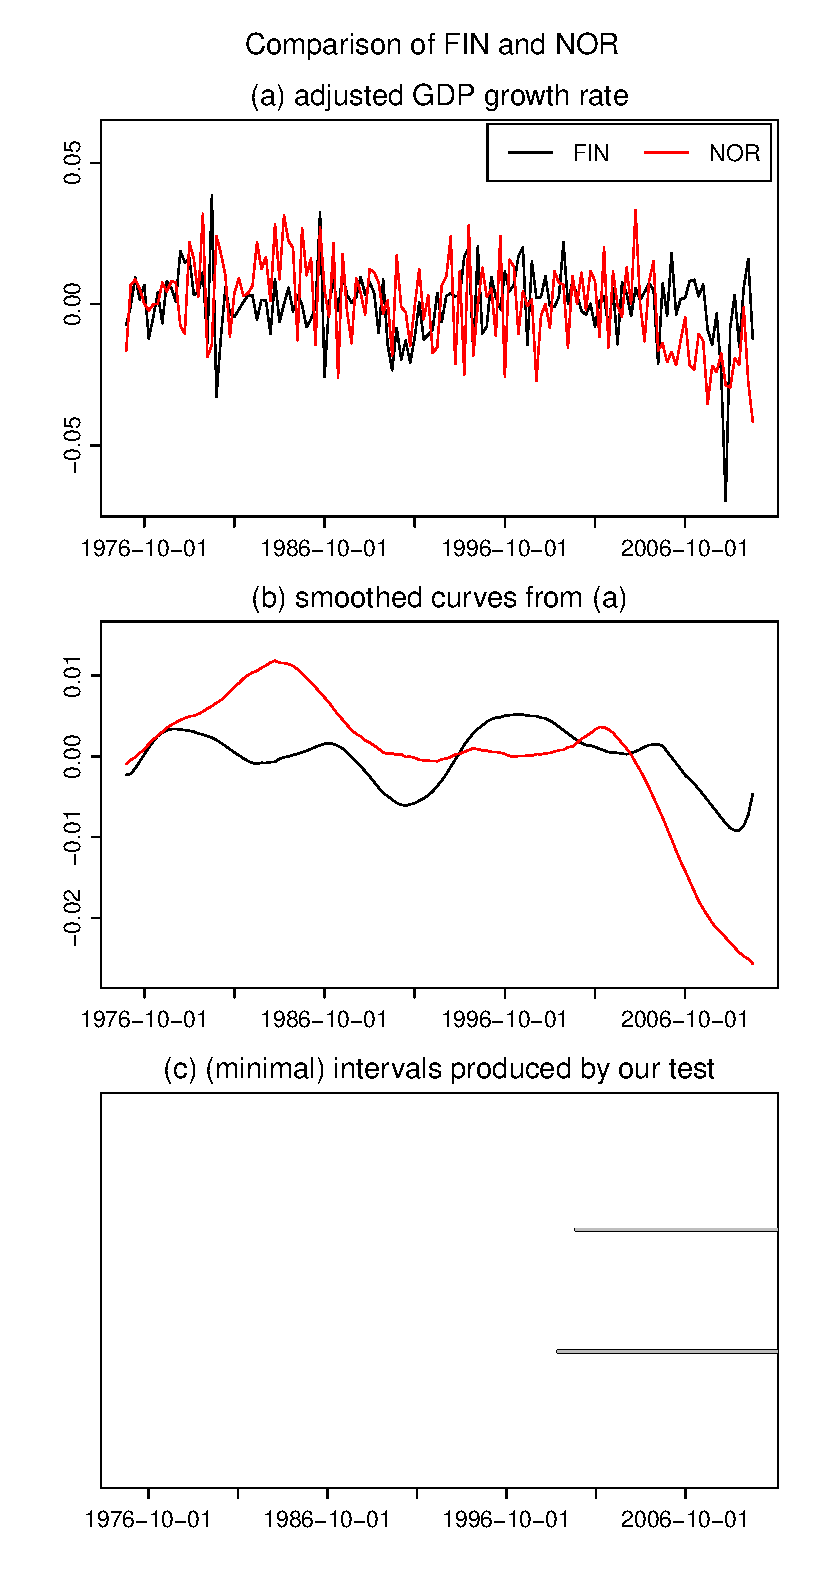
\includegraphics[width=\textwidth]{output/plots/gdp/FIN_vs_NOR}
\caption{Test results for the comparison of Finland and Norway.}\label{fig:Finland:Norway}
\end{minipage}
\hspace{0.1cm}
\begin{minipage}[t]{0.24\textwidth}
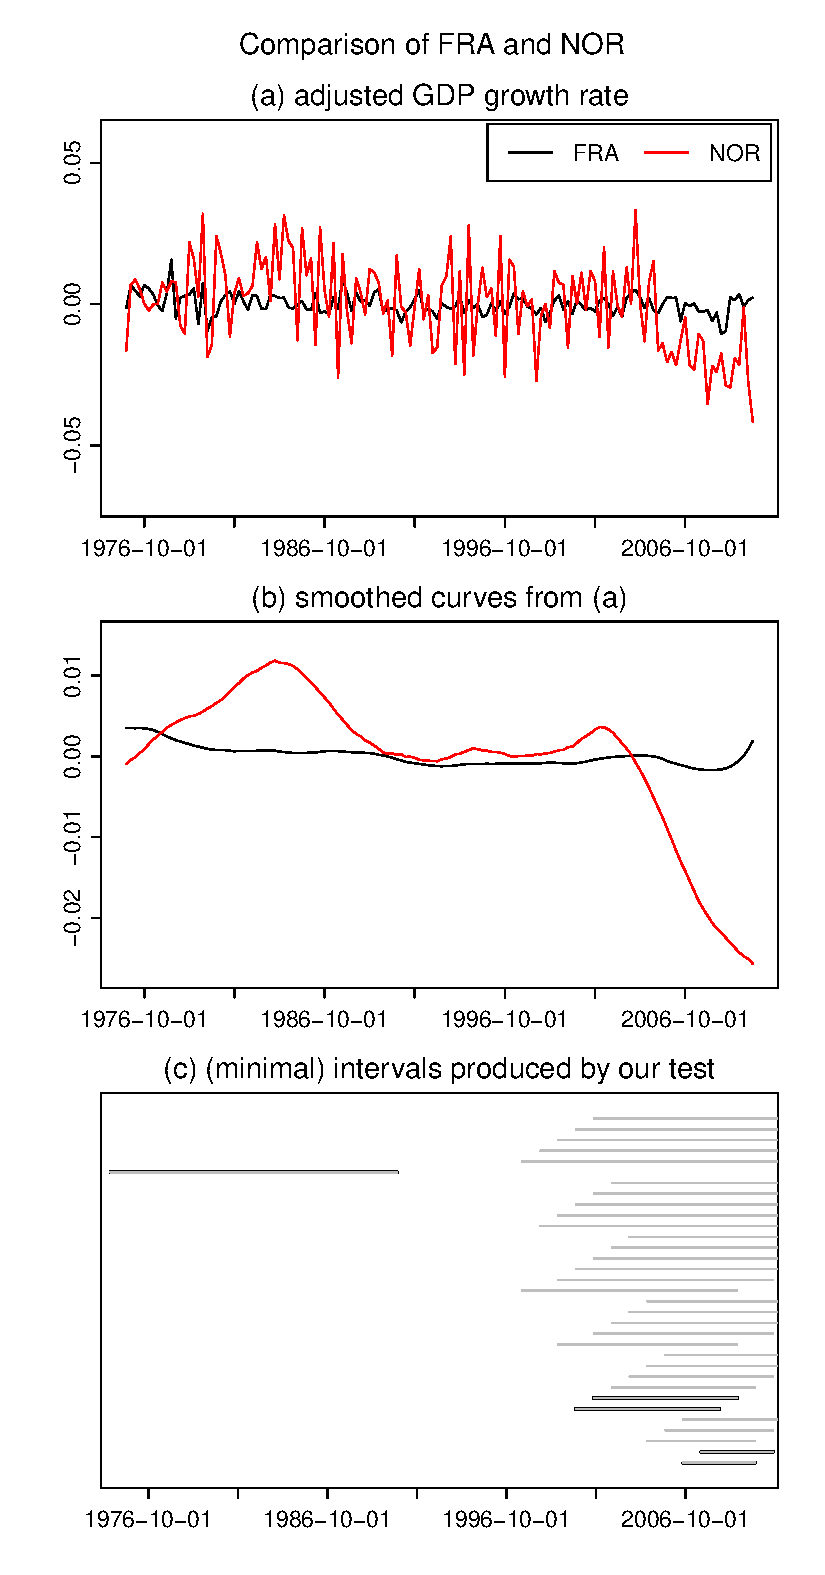
\includegraphics[width=\textwidth]{output/plots/gdp/FRA_vs_NOR}
\caption{Test results for the comparison of France and Norway.}\label{fig:France:Norway}
\end{minipage}
\hspace{0.1cm}
\begin{minipage}[t]{0.24\textwidth}
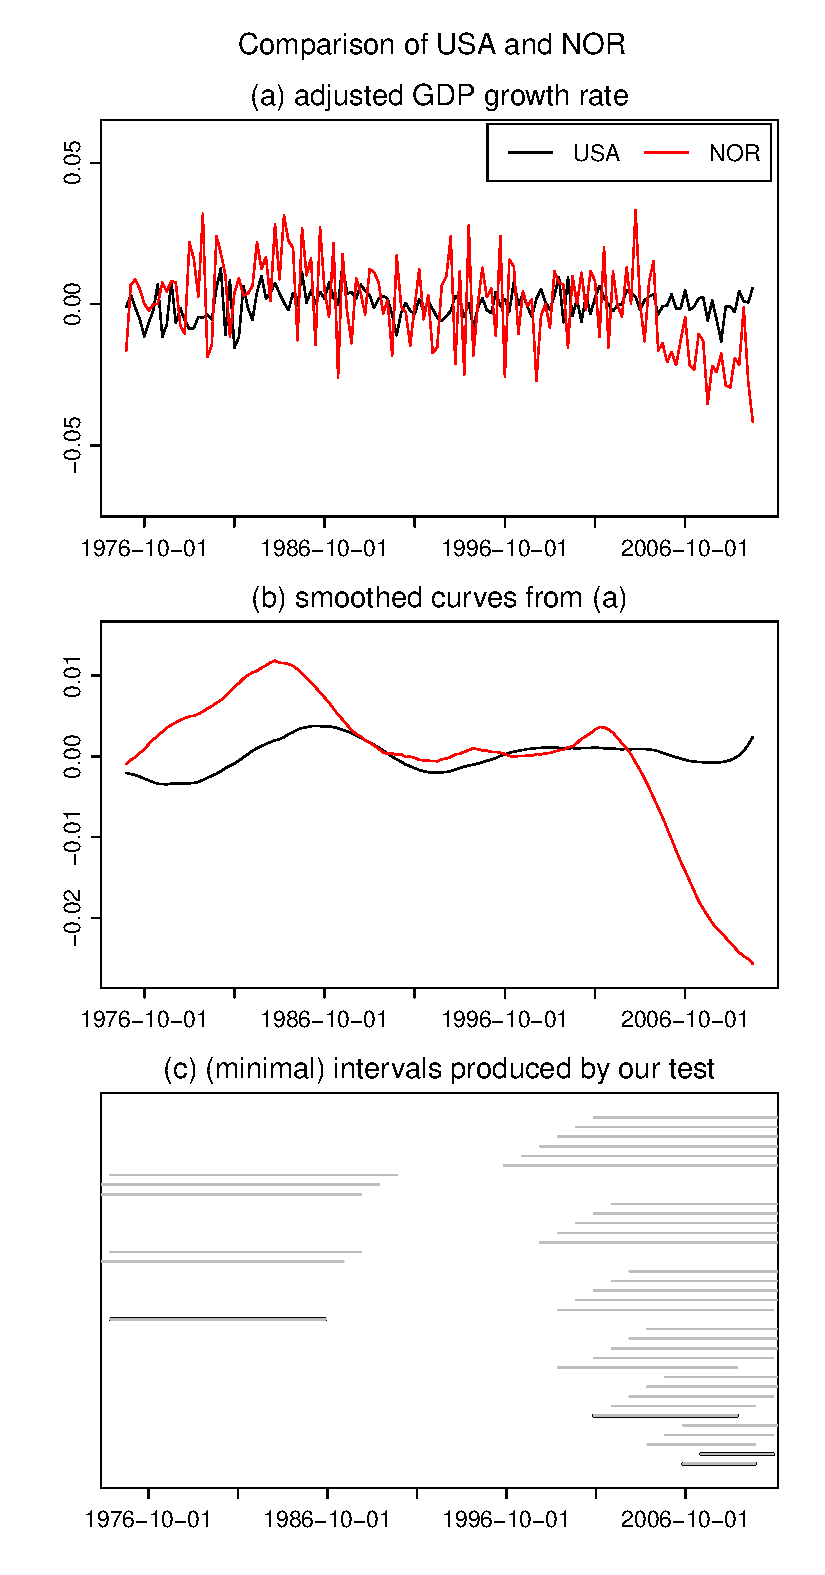
\includegraphics[width=\textwidth]{output/plots/gdp/USA_vs_NOR}
\caption{Test results for the comparison of the USA and Norway.}\label{fig:USA:Norway}
\end{minipage}
\caption*{Note: In each figure, panel (a) shows the two augmented time series, panel (b) presents smoothed versions of the augmented time series, and panel (c) depicts the set of intervals $\mathcal{S}^{[i, j]}(\alpha)$ in grey and the subset of minimal intervals $\mathcal{S}^{[i, j]}_{min}(\alpha)$ in black.}
\end{sidewaysfigure}


\begin{sidewaysfigure}[p!]
\centering
\begin{minipage}[t]{0.24\textwidth}
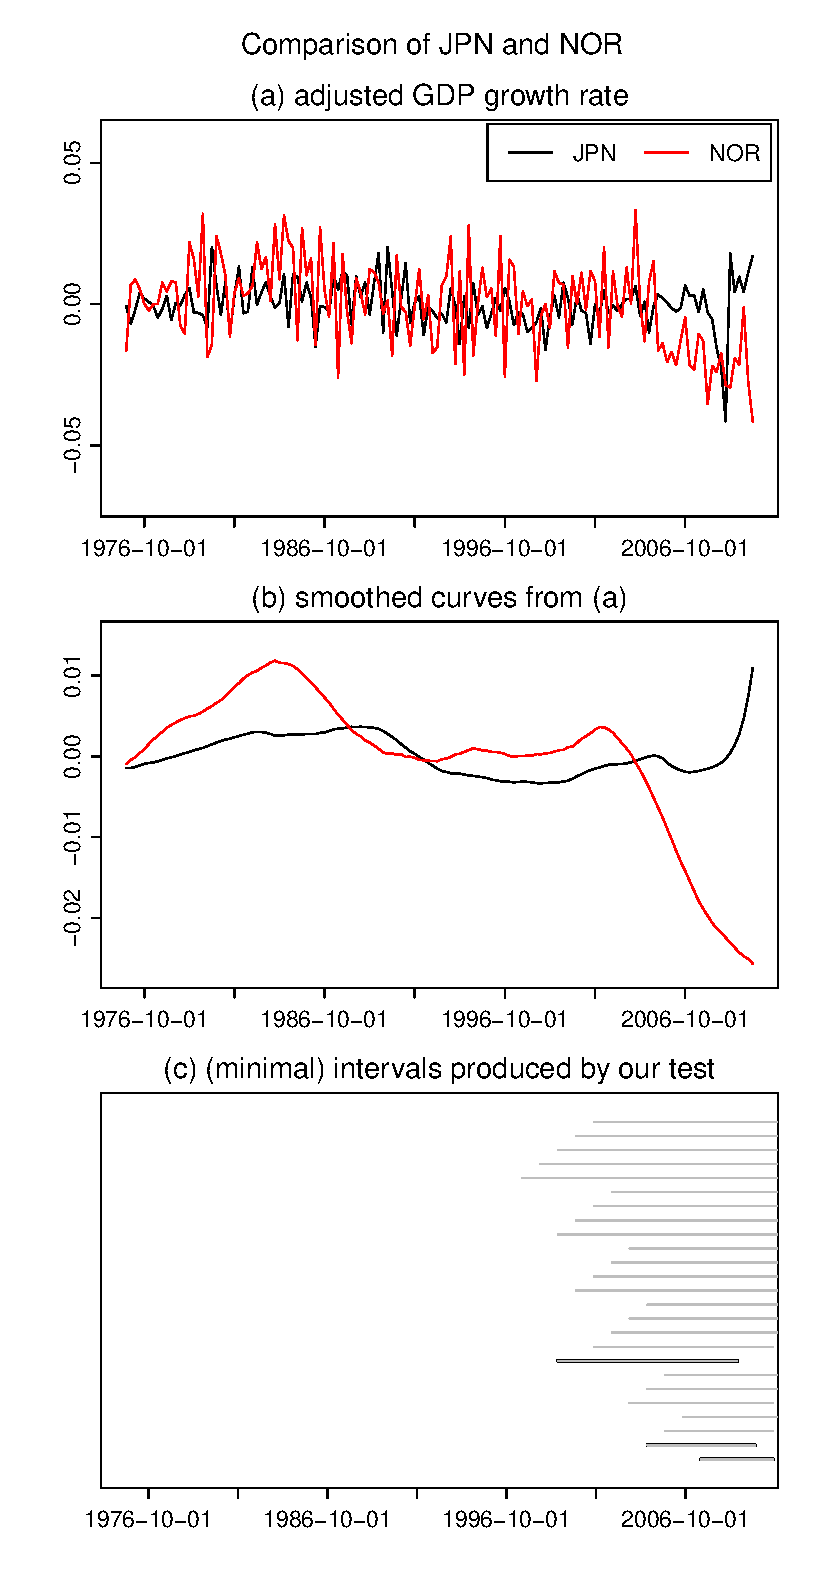
\includegraphics[width=\textwidth]{output/plots/gdp/JPN_vs_NOR}
\caption{Test results for the comparison of Japan and Norway.}\label{fig:Japan:Norway}
\end{minipage}
\hspace{0.1cm}
\begin{minipage}[t]{0.24\textwidth}
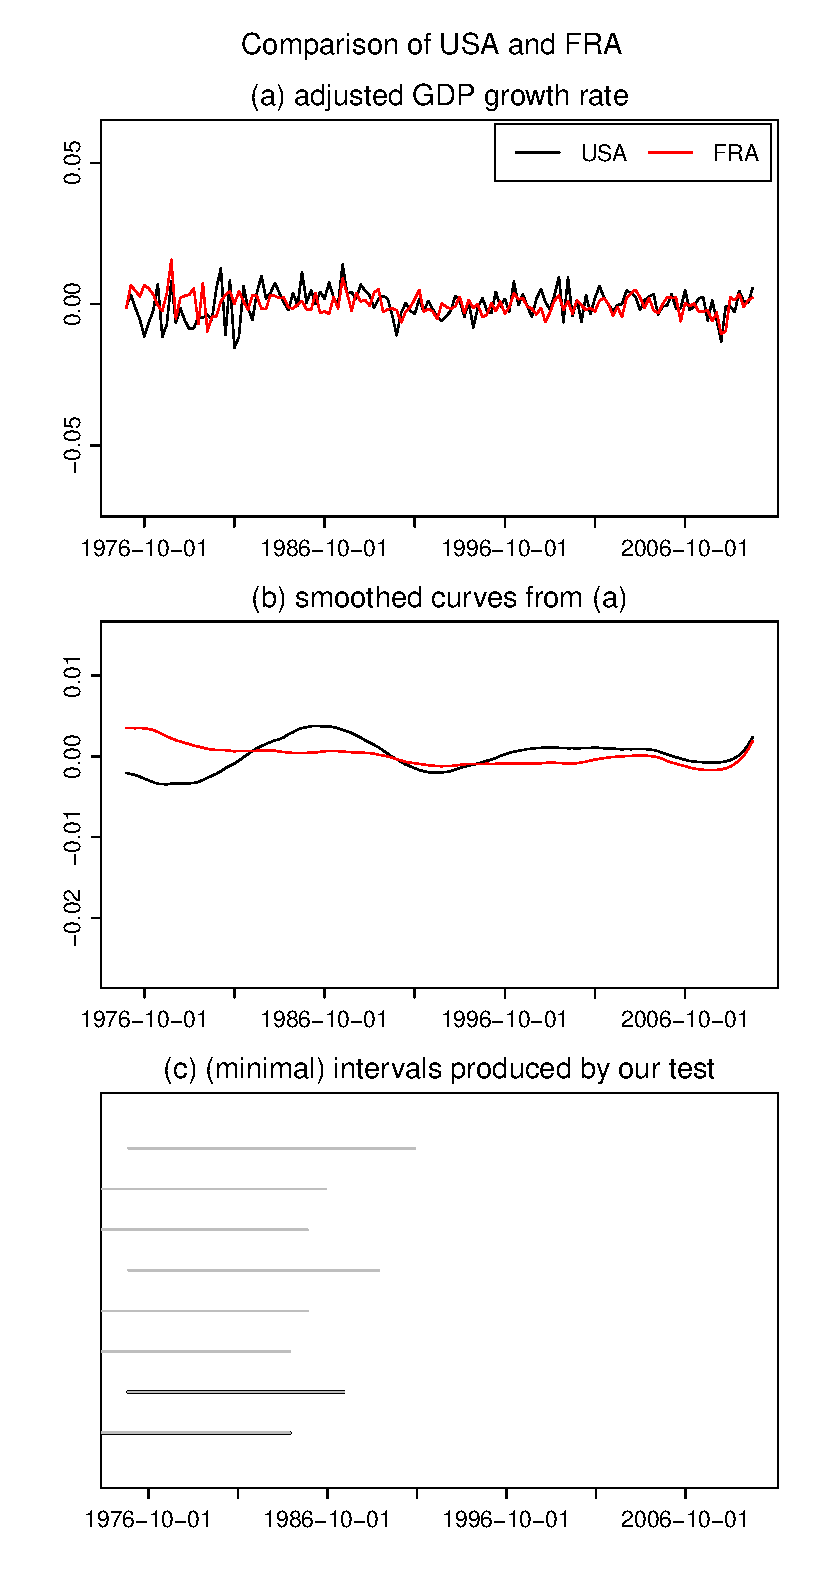
\includegraphics[width=\textwidth]{output/plots/gdp/USA_vs_FRA}
\caption{Test results for the comparison of the USA and France.}\label{fig:USA:France}
\end{minipage}
\hspace{0.1cm}
\begin{minipage}[t]{0.24\textwidth}
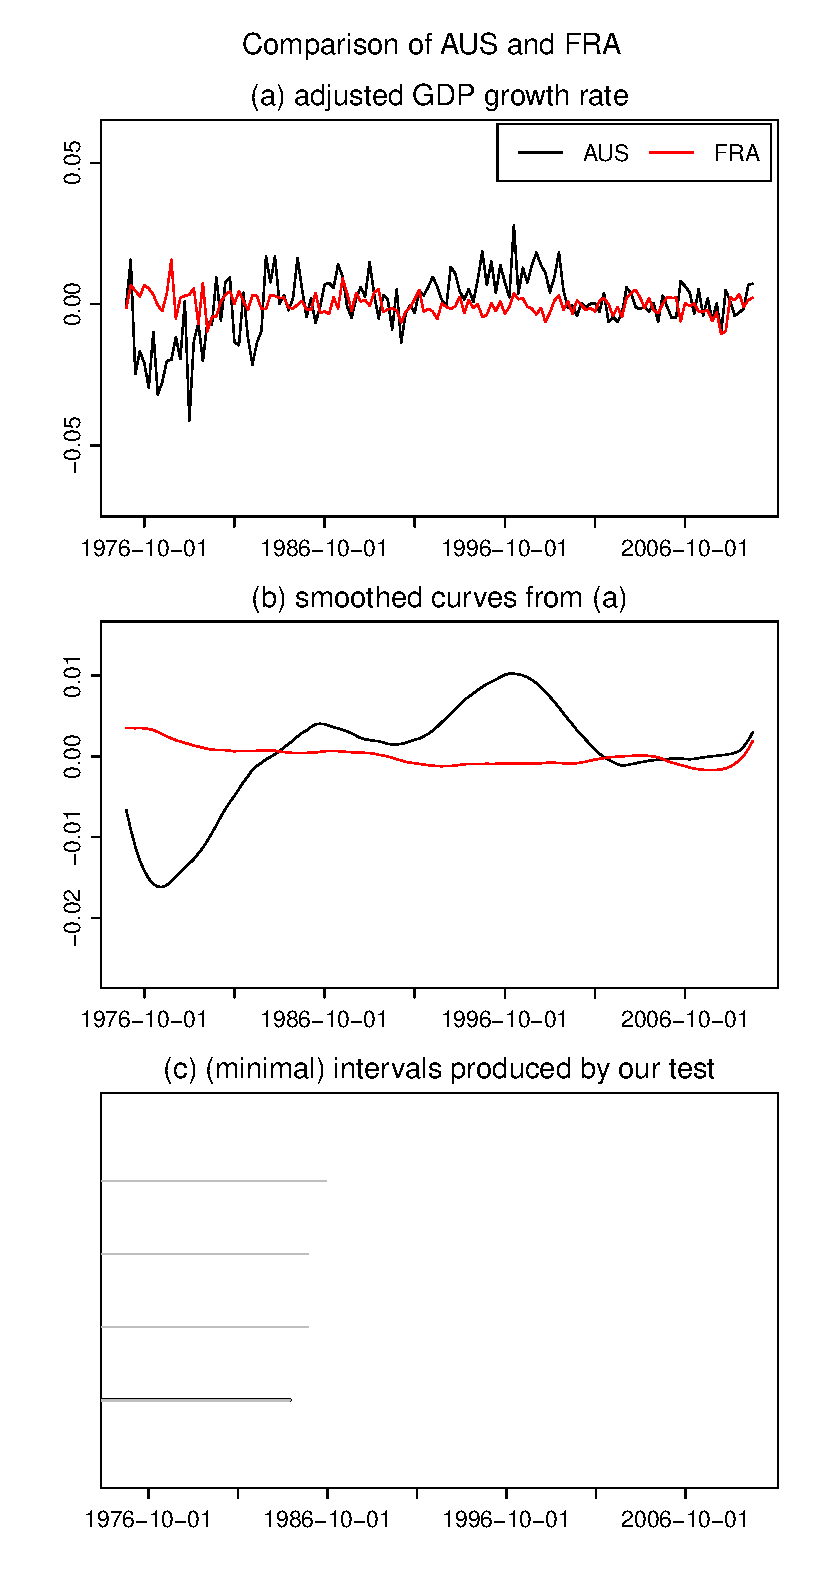
\includegraphics[width=\textwidth]{output/plots/gdp/AUS_vs_FRA}
\caption{Test results for the comparison of Australia and France.}\label{fig:Australia:France}
\end{minipage}
\caption*{Note: In each figure, panel (a) shows the two augmented time series, panel (b) presents smoothed versions of the augmented time series, and panel (c) depicts the set of intervals $\mathcal{S}^{[i, j]}(\alpha)$ in grey and the subset of minimal intervals $\mathcal{S}^{[i, j]}_{min}(\alpha)$ in black.}
\end{sidewaysfigure}


Out of $55$ pairwise comparisons, our test detects differences for $11$ pairs of countries $(i,j)$. These $11$ cases are presented in Figures~\ref{fig:Australia:Norway}--\ref{fig:Australia:France}. In $9$ cases (Figures \ref{fig:Australia:Norway}--\ref{fig:Japan:Norway}), one of the involved countries is Norway. Inspecting the trend estimates in panels (b) of Figures \ref{fig:Australia:Norway}--\ref{fig:Japan:Norway}, the Norwegian trend estimate can be seen to exhibit a strong downward movement at the end of the observation period, whereas the other trend estimates show a much less pronounced downward movement (or even a slight upward movement). According to our test, this is a significant difference between the Norwegian and the other trend functions rather than an artefact of the sampling noise: In all $9$ cases, the test rejects the local null for at least one interval which covers the last $10$ years of the analysed time period (from the first quarter in $2000$ up to the third quarter in $2010$). Apart from these differences at the end of the sampling period, our test also finds differences in the beginning, however, only for part of the pairwise comparisons. 


Figures \ref{fig:USA:France} and \ref{fig:Australia:France} present the results of the pairwise comparison between Australia and France and between the USA and France, respectively. In both cases, our test detects differences between the GDP trends only in the beginning of the considered time period. In the case of Australia and France, it is clearly visible in the raw data (panel (a) in Figure~\ref{fig:Australia:France}) that there is a difference between the trends, whereas this is not so obvious in the case of the USA and France. According to our test, there are indeed significant differences in both cases. In particular, we can claim with confidence at least 95\%, that there are differences between the trends of the USA and France (of Australia and France) up to the fourth quarter in 1991 (the fourth quarter in 1986), but there is no evidence of any differences between the trends from 1992 (1987) onwards.


\begin{figure}[t!]
\begin{center}
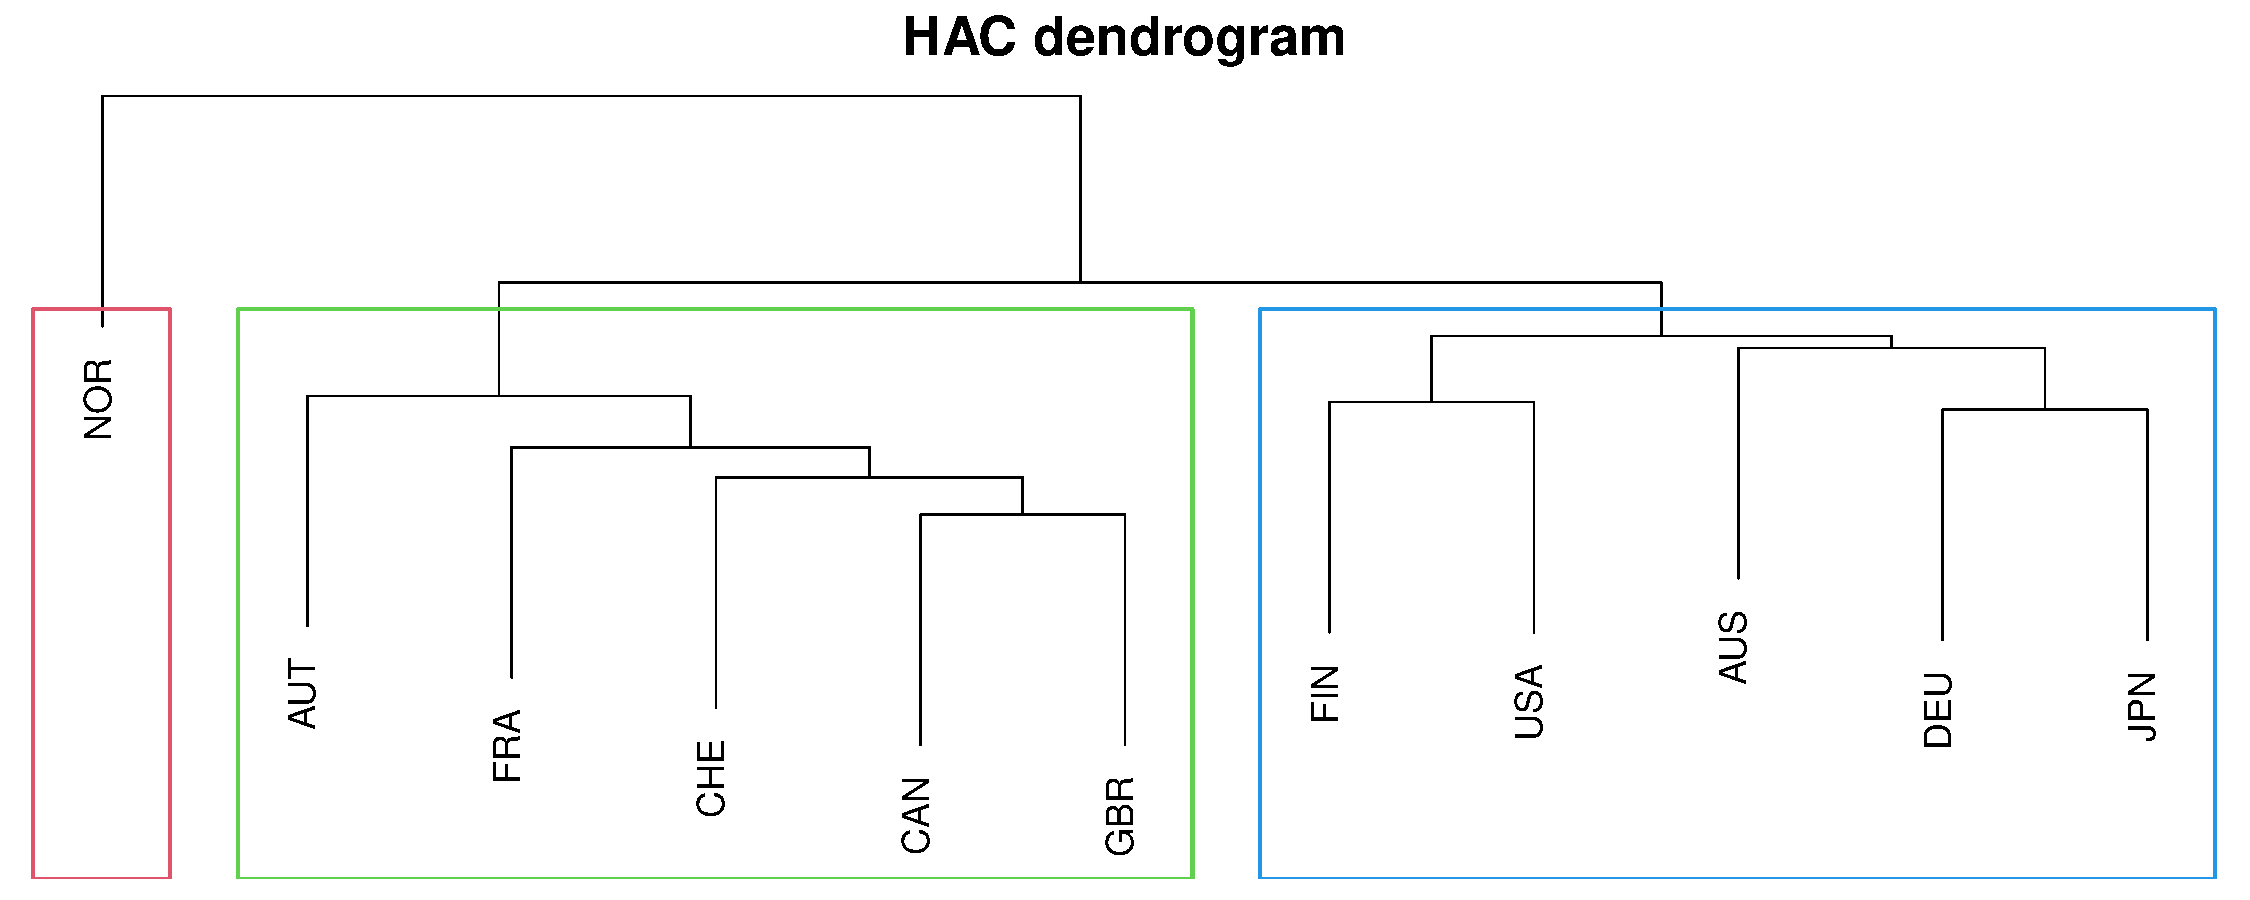
\includegraphics[width=0.75\textwidth]{output/plots/gdp/dendrogram}
\caption{Dendrogram of the HAC algorithm. Each coloured rectangle corresponds to one of the clusters.}\label{fig:gdp:dend}

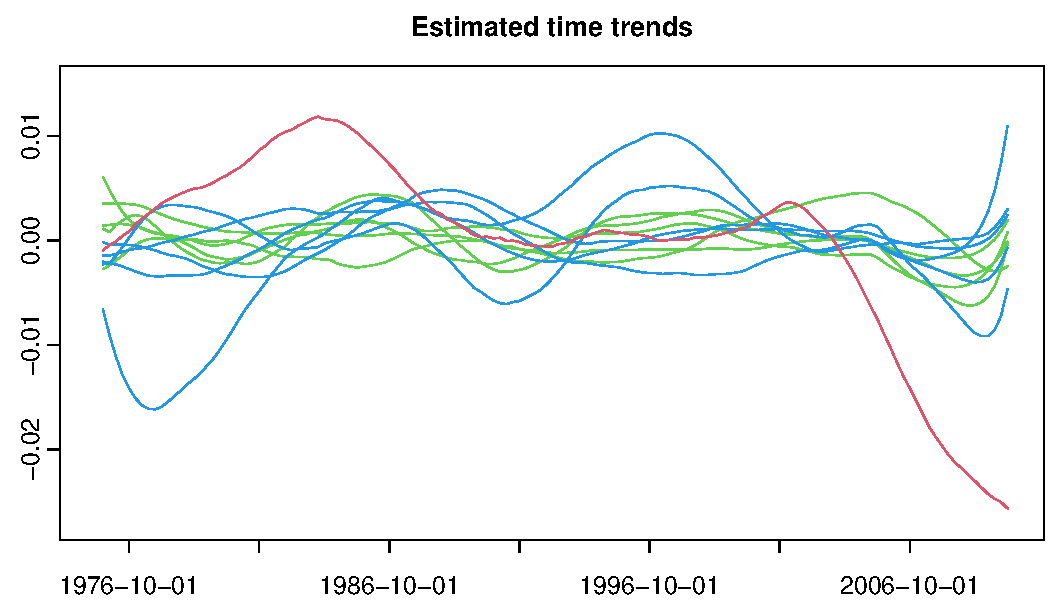
\includegraphics[width=0.75\textwidth]{output/plots/gdp/all_clusters}
\caption{Local linear estimates of the $n=11$ time trends (calculated from the augmented time series $\widehat{Y}_{it}$ with bandwidth $h = 0.1$ and Epanechnikov kernel). Each trend estimate is coloured according to the cluster that it is assigned to. }\label{fig:gdp:all_clusters}
\end{center}
\end{figure}


We next apply our clustering techniques to find groups of countries that have the same time trend. We implement our HAC algorithm with $\alpha = 0.05$ and the same choices as detailed above. The dendrogram that depicts the clustering results is plotted in Figure \ref{fig:gdp:dend}. The number of clusters is estimated to be $\widehat{N} = 3$. The rectangles in Figure \ref{fig:gdp:dend} indicate the $\widehat{N} = 3$ clusters. In particular, each rectangle is drawn around the branches of the dendrogram that correspond to one of the three clusters. Figure \ref{fig:gdp:all_clusters} depicts local linear kernel estimates of the $n=11$ GDP time trends (calculated from the augmented time series $\widehat{Y}_{it}$ with bandwidth $0.1$ and Epanechnikov kernel). Their colour indicates which cluster they belong to. 


The results in Figures \ref{fig:gdp:dend} and \ref{fig:gdp:all_clusters} show that there is one cluster which consists only of Norway (plotted in red). As we have already discussed above and as becomes apparent from Figure \ref{fig:gdp:all_clusters}, the Norwegian trend exhibits a strong downward movement at the end of the sampling period, whereas the other trends show a much more moderate downward movement (if at all). This is presumably the reason why the clustering procedure puts Norway in a separate cluster. The algorithm further finds two other clusters, one consisting of the 5 countries Australia, Finland, Germany, Japan and the USA (plotted in blue in Figures \ref{fig:gdp:dend} and \ref{fig:gdp:all_clusters}) and the other one consisting of the 5 countries Austria, Canada, France, Switzerland and the UK (plotted in  green in Figures \ref{fig:gdp:dend} and \ref{fig:gdp:all_clusters}). Visual inspection of the trend estimates in Figure \ref{fig:gdp:all_clusters} suggests that the GDP time trends in the blue cluster exhibit more pronounced decreases and increases than the GDP time trends in the green cluster. Hence, overall, the clustering procedure appears to produce a reasonable grouping of the GDP trends.
 


\section{Technical details}\label{appendix}


In what follows, we prove the theoretical results from Sections \ref{sec:theo} and \ref{sec:clustering}. We use the following notation: The symbol $C$ denotes a universal real constant which may take a different value on each occurrence. For $a,b \in \reals$, we write $a \vee b = \max\{a,b\}$. For $x \in \reals_{\geq 0}$, we let $\lfloor x \rfloor$ denote the integer value of $x$ and $\lceil x \rceil$ the smallest integer greater than or equal to $x$. For any set $A$, the symbol $|A|$ denotes the cardinality of $A$. The expression $X \stackrel{\mathcal{D}}{=} Y$ means that the two random variables $X$ and $Y$ have the same distribution. Finally, we sometimes use the notation $a_T \ll b_T$ to express that $a_T = o(b_T)$. 



\enlargethispage{0.25cm}
\subsection*{Auxiliary results}\label{subsec:appendix:aux}


Let $\{Z_t\}_{t=-\infty}^\infty$ be a stationary time series process with $Z_t \in \mathcal{L}^q$ for some $q > 2$ and $\ex[Z_t] = 0$. Assume that $Z_t$ can be represented as $Z_t = g(\ldots, \eta_{t-1}, \eta_t)$, where $\eta_t$ are i.i.d.\ variables and $g: \reals^\infty \to \reals$ is a measurable function. We first state a Nagaev-type inequality from \cite{Wu2016}. 


\begin{definitionA}\label{defA-DAN} 
Let $q > 0$ and $\alpha > 0$. The dependence adjusted norm of the process $Z. = \{Z_t\}_{t=-\infty}^\infty$ is given by 
$\|Z.\|_{q, \alpha} = \sup_{t\geq 0} (t+1)^{\alpha} \sum_{s=t}^{\infty} \delta_{q}(g,s)$.
\end{definitionA}


\begin{propA}[\cite{Wu2016}, Theorem 2]\label{theo-wu2016}
Assume that $\|Z.\|_{q, \alpha} < \infty$ with $q > 2$ and $\alpha > 1/2 - 1/q$. Let $S_T = a_1 Z_1 + \ldots + a_T Z_T$, where $a_1,\ldots,a_T$ are real numbers with $\sum_{t=1}^T a_t^2 = T$. Then for any $w>0$,
\[ \pr(|S_T| \geq w) \leq C_1 \frac{|a|_{q}^{q}\|Z.\|^{q}_{q, \alpha}}{w^{q}} + C_2 \exp \left( - \frac{C_3 w^2} {T \|Z.\|^2_{2, \alpha}}\right), \]
where $C_1, C_2, C_3$ are constants that only depend on $q$ and $\alpha$.
\end{propA}


The following lemma is a simple consequence of the above inequality. 


\begin{lemmaA}\label{lemma-wlln}
Let $\sum_{s=t}^\infty \delta_{q}(g,s) = O(t^{-\alpha})$ for some $q > 2$ and $\alpha > 1/2 - 1/q$. Then 
\[ \frac{1}{\sqrt{T}} \sum_{t=1}^T Z_t = O_p(1). \]
\end{lemmaA} 


\begin{proof}[\textnormal{\textbf{Proof of Lemma \ref{lemma-wlln}.}}]
Let $\eta > 0$ be a fixed number. We apply Proposition \ref{theo-wu2016} to the sum $S_T = \sum_{t=1}^T a_t Z_t$ with $a_t = 1$ for all $t$. The assumption $\sum_{s=t}^\infty \delta_{q}(g,s) = O(t^{-\alpha})$ implies that $\|Z.\|_{2, \alpha} \le \|Z.\|_{q, \alpha} \le C_Z < \infty$. Hence, for $w$ chosen sufficiently large, we get 
\begin{align*}
\pr\Big( \Big| \sum_{t=1}^T Z_t \Big| \geq \sqrt{T} w\Big) 
 & \leq C_1 \frac{T C_Z^q}{T^{q/2} w^q} + C_2 \exp \left( - \frac{C_3 T w^2} {T C_Z^2}\right) \\
 & = \frac{\{C_1 C_Z^q\} T^{1-q/2}}{w^q} + C_2 \exp \left( - \frac{C_3 w^2} {C_Z^2}\right) \le \eta
\end{align*}
for all $T$. This means that $\sum_{t=1}^T Z_t / \sqrt{T} = O_p(1)$. 
\end{proof}


Let $\Delta \varepsilon_{it} = \varepsilon_{it} - \varepsilon_{it-1}$ and $\Delta \X_{it} = \X_{it} - \X_{it-1}$. By Assumptions \ref{C-err1} and \ref{C-reg1}, $\Delta \varepsilon_{it} = \Delta g_i(\mathcal{F}_{it})$ and $\Delta \X_{it} = \Delta \boldsymbol{h}_{i}(\mathcal{G}_{it})$. We further define
\begin{align*}
\boldsymbol{a}_{i}(\mathcal{H}_{it}) & := \Delta \boldsymbol{h}_{i}(\mathcal{G}_{it}) \Delta g_i(\mathcal{F}_{it})\phantom{^\top} = \Delta \X_{it} \Delta \varepsilon_{it} \\
\boldsymbol{b}_{i}(\mathcal{G}_{it}) & := \Delta \boldsymbol{h}_{i}(\mathcal{G}_{it}) \Delta \boldsymbol{h}_{i}(\mathcal{G}_{it})^\top = \Delta \X_{it} \Delta \X_{it}^\top,
\end{align*}
where $\boldsymbol{a}_i = (a_{ij})_{j=1}^d$, $\boldsymbol{b}_i = (b_{ikl})_{k,l=1}^d$ and $\mathcal{H}_{it} = (\mathcal{H}_{it,1},\ldots,\mathcal{H}_{it,d})^\top$ with $\mathcal{H}_{it,j} = (\ldots, \nu_{it-1,j},\linebreak \nu_{it,j})$ and $\nu_{it,j} = (\eta_{it},\xi_{it,j})$. The next result gives bounds on the physical dependence measures of the processes $\{ \boldsymbol{a}_{i}(\mathcal{H}_{it}) \}_{t=-\infty}^\infty$ and $\{ \boldsymbol{b}_{i}(\mathcal{G}_{it}) \}_{t=-\infty}^\infty$. 


\begin{lemmaA}\label{lemma-bounds-dep-measure}
Let Assumptions \ref{C-err1}, \ref{C-err3}, \ref{C-reg1} and \ref{C-reg3} be satisfied. Then for each $i$, $j$, $k$ and $l$, it holds that
\begin{align*}
 & \sum_{s=t}^\infty \delta_p(a_{ij}, s) = O(t^{-\alpha}) \, \qquad \text{for } p = \min\{q,q^\prime\}/2 \text{ and some } \alpha > 1/2 - 1/p \\
 & \sum_{s=t}^\infty \delta_p(b_{ikl}, s) = O(t^{-\alpha}) \qquad \text{for } p = q^\prime/2 \text{ and some } \alpha > 1/2 - 1/p.
\end{align*}
\end{lemmaA}


\begin{proof}[\textnormal{\textbf{Proof of Lemma \ref{lemma-bounds-dep-measure}.}}]
We only prove the first statement. The second one follows by analogous arguments. By the definition of the physical dependence measure and the Cauchy-Schwarz inequality, we have with $p = \min\{q,q^\prime\}/2$ that
\begin{align*}
\delta_p(a_{ij}, s) 
 & = \| a_{ij}(\mathcal{H}_{it,j}) - a_{ij}(\mathcal{H}_{it,j}^\prime) \|_p \\
 &= \| \Delta h_{ij}(\mathcal{G}_{it}) \Delta g_i(\mathcal{F}_{it}) -  \Delta h_{ij}(\mathcal{G}_{it}^\prime) \Delta g_i(\mathcal{F}_{it}^\prime) \|_p \\
 &\leq \| h_{ij}(\mathcal{G}_{it}) g_i(\mathcal{F}_{it}) - h_{ij}(\mathcal{G}_{it}^\prime) g_i(\mathcal{F}_{it}^\prime) \|_p \\
 &\quad + \| h_{ij}(\mathcal{G}_{it-1}) g_i(\mathcal{F}_{it-1}) - h_{ij}(\mathcal{G}_{it-1}^\prime) g_i(\mathcal{F}_{it-1}^\prime) \|_p \\
 &\quad + \| h_{ij}(\mathcal{G}_{it-1}) g_i(\mathcal{F}_{it}) - h_{ij}(\mathcal{G}_{it-1}^\prime) g_i(\mathcal{F}_{it}^\prime) \|_p \\
 &\quad + \| h_{ij}(\mathcal{G}_{it}) g_i(\mathcal{F}_{it-1}) - h_{ij}(\mathcal{G}_{it}^\prime) g_i(\mathcal{F}_{it-1}^\prime) \|_p \\
 & = \| \{ h_{ij}(\mathcal{G}_{it}) - h_{ij}(\mathcal{G}_{it}^\prime)\} g_i(\mathcal{F}_{it}) + h_{ij}(\mathcal{G}_{it}^\prime) \{g_i(\mathcal{F}_{it}) - g_i(\mathcal{F}_{it}^\prime)\} \|_p \\
 & \quad + \| \{ h_{ij}(\mathcal{G}_{it-1}) - h_{ij}(\mathcal{G}_{it-1}^\prime)\} g_i(\mathcal{F}_{it-1}) + h_{ij}(\mathcal{G}_{it-1}^\prime) \{g_i(\mathcal{F}_{it-1}) - g_i(\mathcal{F}_{it-1}^\prime)\} \|_p \\
 &\quad + \| \{ h_{ij}(\mathcal{G}_{it-1}) - h_{ij}(\mathcal{G}_{it-1}^\prime)\} g_i(\mathcal{F}_{it}) + h_{ij}(\mathcal{G}_{it-1}^\prime) \{g_i(\mathcal{F}_{it}) - g_i(\mathcal{F}_{it}^\prime)\} \|_p \\
 &\quad + \| \{ h_{ij}(\mathcal{G}_{it}) - h_{ij}(\mathcal{G}_{it}^\prime)\} g_i(\mathcal{F}_{it-1}) + h_{ij}(\mathcal{G}_{it}^\prime) \{g_i(\mathcal{F}_{it-1}) - g_i(\mathcal{F}_{it-1}^\prime)\} \|_p \\
 &\leq \delta_{2p}(h_{ij}, t) \| g_i(\mathcal{F}_t) \|_{2p} + \delta_{2p} (g_i, t) \| h_{ij}(\mathcal{G}_{it}^\prime) \|_{2p} \\
&\quad + \delta_{2p}(h_{ij}, t-1) \| g_i(\mathcal{F}_{t-1}) \|_{2p} + \delta_{2p} (g_i, t-1) \| h_{ij}(\mathcal{G}_{it-1}^\prime) \|_{2p} \\
&\quad + \delta_{2p}(h_{ij}, t-1) \| g_i(\mathcal{F}_t) \|_{2p} + \delta_{2p} (g_i, t) \| h_{ij}(\mathcal{G}_{it-1}^\prime) \|_{2p} \\
&\quad + \delta_{2p}(h_{ij}, t) \| g_i(\mathcal{F}_{t-1}) \|_{2p} + \delta_{2p} (g_i, t-1) \| h_{ij}(\mathcal{G}_{it}^\prime) \|_{2p}, 
\end{align*}
where $\mathcal{H}_{it,j}^\prime  = (\ldots, \nu_{i(-1),j}, \nu^\prime_{i0,j}, \nu_{i1,j}, \ldots, \nu_{it-1,j}, \nu_{it,j})$, $\mathcal{G}_{it,j}^\prime  = (\ldots, \xi_{i(-1),j}, \xi^\prime_{i0,j}, \xi_{i1,j}, \ldots, \linebreak \xi_{it-1,j}, \xi_{it,j})$ and $\mathcal{F}_{it}^\prime  = (\ldots, \eta_{i(-1)}, \eta^\prime_{i0}, \eta_{i1}, \ldots, \eta_{it-1}, \eta_{it})$ are coupled processes with $\nu_{i0,j}^\prime$, $\xi_{i0,j}^\prime$ and $\eta_{i0,j}^\prime$ being i.i.d.\ copies of $\nu_{i0,j}$, $\xi_{i0,j}$ and $\eta_{i0}$. From this and Assumptions \ref{C-err1}, \ref{C-err3}, \ref{C-reg1} and \ref{C-reg3}, it immediately follows that $\sum_{s=t}^\infty \delta_p(a_{ij}, s) = O(t^{-\alpha})$.
\end{proof}


We now show that the estimator $\widehat{\bfbeta}_i$ is $\sqrt{T}$-consistent for each $i$ under our conditions.


\begin{lemmaA}\label{lemma-beta-rate}
Let Assumptions \ref{C-err1}, \ref{C-err3} and \ref{C-reg1}--\ref{C-reg-err} be satisfied. Then for each $i$, it holds that
\[ \widehat{\bfbeta}_i - \bfbeta_i = O_p\Big(\frac{1}{\sqrt{T}}\Big). \]
\end{lemmaA}


\begin{proof}[\textnormal{\textbf{Proof of Lemma \ref{lemma-beta-rate}.}}]
The estimator $\widehat{\bfbeta}_i$ can be written as
\begin{align*}
\widehat{\bfbeta}_i &= \Big( \sum_{t=2}^T \Delta \X_{it} \Delta \X_{it}^\top \Big)^{-1} \sum_{t=2}^T \Delta \X_{it} \Delta Y_{it} \\
& =  \Big( \sum_{t=2}^T \Delta \X_{it} \Delta \X_{it}^\top \Big)^{-1} \sum_{t=2}^T \Delta \X_{it} \bigg(\Delta \X_{it}^\top \bfbeta_i +  \Delta m_{it}+ \Delta \varepsilon_{it} \bigg) \\
&= \bfbeta_i + \Big( \sum_{t=2}^T \Delta \X_{it} \Delta \X_{it}^\top \Big)^{-1} \sum_{t=2}^T \Delta \X_{it} \Delta m_{it} +  \Big( \sum_{t=2}^T \Delta \X_{it} \Delta \X_{it}^\top \Big)^{-1} \sum_{t=2}^T \Delta \X_{it} \Delta \varepsilon_{it}, 
\end{align*}
where $\Delta \X_{it} = \X_{it} - \X_{it-1}$, $\Delta \varepsilon_{it} = \varepsilon_{it} - \varepsilon_{it-1}$ and $\Delta m_{it} = m_i (\frac{t}{T}) - m_i(\frac{t-1}{T})$. Hence, 
\begin{align}
 \sqrt{T}( \widehat{\bfbeta}_i - \bfbeta_i) = &\Big( \frac{1}{T}\sum_{t=2}^T \Delta \X_{it} \Delta \X_{it}^\top \Big)^{-1} \frac{1}{\sqrt{T}}\sum_{t=2}^T \Delta \X_{it} \Delta m_{it} \nonumber \\
&\quad+  \Big(\frac{1}{T} \sum_{t=2}^T \Delta \X_{it} \Delta \X_{it}^\top \Big)^{-1}\frac{1}{\sqrt{T}} \sum_{t=2}^T \Delta \X_{it} \Delta \varepsilon_{it}. \label{theo:beta:proof1}
\end{align}
In what follows, we show that 
\begin{align}
\frac{1}{\sqrt{T}} \sum_{t=2}^T \Delta \X_{it} \Delta \varepsilon_{it} & = O_p(1) \label{lemma-beta-rate-claim1} \\
\Big( \frac{1}{T}\sum_{t=2}^T \Delta \X_{it} \Delta \X_{it}^\top \Big)^{-1} & = O_p(1) \label{lemma-beta-rate-claim2} \\
\frac{1}{\sqrt{T}} \sum_{t=2}^T \Delta \X_{it} \Delta m_{it} & = O_p\Big(\frac{1}{\sqrt{T}}\Big). \label{lemma-beta-rate-claim3}
\end{align} 
Lemma \ref{lemma-beta-rate} follows from applying these three statements together with standard arguments to formula \eqref{theo:beta:proof1}.


Since $\ex[\Delta \X_{it} \Delta \varepsilon_{it}] = 0$ by \ref{C-reg-err} and $\sum_{s=t}^\infty \delta_p(a_{ij}, s) = O(t^{-\alpha})$ for some $p > 2$, $\alpha > 1/2 - 1/p$ and all $j$ by Lemma \ref{lemma-bounds-dep-measure}, the claim \eqref{lemma-beta-rate-claim1} follows upon applying Lemma \ref{lemma-wlln}. Another application of Lemma \ref{lemma-wlln} yields that 
\[ \frac{1}{T}\sum_{t=2}^T \Big\{ \Delta \X_{it} \Delta \X_{it}^\top - \ex[\Delta \X_{it} \Delta \X_{it}^\top] \Big\} = O_p\Big(\frac{1}{\sqrt{T}}\Big). \]
As $\ex[\Delta \X_{it} \Delta \X_{it}^\top]$ is invertible, we can invoke Slutsky's lemma to obtain \eqref{lemma-beta-rate-claim2}. By assumption, $m_i$ is Lipschitz continuous, which implies that $|\Delta m_{it}| = |m_i (\frac{t}{T}) - m_i (\frac{t-1}{T}) | \leq C/T$ for all $t \in \{1, \ldots, T\}$ and some constant $C > 0$. Hence, 
\begin{align*}
\Big| \frac{1}{\sqrt{T}}\sum_{t=2}^T \Delta X_{it,j} \Delta m_{it}\Big| &\leq \frac{1}{\sqrt{T}}\sum_{t=2}^T \big|\Delta X_{it,j} \big| \cdot \big| \Delta m_{it} \big| \\
	& \leq \frac{C}{\sqrt{T}} \cdot \frac{1}{T} \sum_{t=2}^T \left|\Delta X_{it,j} \right| = O_p\Big(\frac{1}{\sqrt{T}}\Big),
\end{align*}
where we have used that $T^{-1} \sum_{t=2}^T |\Delta X_{it,j}| = O_p(1)$ by Markov's inequality. This yields \eqref{lemma-beta-rate-claim3}.
\end{proof}


{\color{red}
\begin{lemmaA}\label{lemmaA:lrv}
Let
\begin{align*}
\widehat{\sigma}_i^2 = \frac{1}{2(M-1)s_T}\sum_{m=1}^M \bigg[ \sum_{t = 1}^{s_T} & \Big(Y_{i(t + ms_T)} - Y_{i(t + (m-1)s_T)} \\[-0.2cm] & - \widehat{\bfbeta}_i^\top\big(\X_{i(t+ms_T)} - \X_{i(t+(m-1)s_T)}\big) \Big)\bigg]^2, 
\end{align*}
be the subseries estimator of $\sigma_i^2$, where $s_T \asymp T^{1/3}$ is the length of the subseries and $M = \lfloor T/s_T\rfloor$ is the largest integer not exceeding $T/s_T$. Under Assumptions \ref{C-err1}--\ref{C-reg-err}, 
$$\widehat{\sigma}_i^2 = \sigma_i^2 + O_p(T^{-1/3})$$
for each $i$.
\end{lemmaA}}


\begin{proof}[\textnormal{\textbf{Proof of Lemma \ref{lemmaA:lrv}}}]
%For notational convenience, we let $Y_{it}^* = Y_{it} - \bfbeta_i^\top \X_{it}$. Note that 
%\begin{align*}
%&Y_{i(t + ms_T)}^* - Y_{i(t + (m-1)s_T)}^* \\
%&= \alpha_i + m_i\left(\frac{t+m s_T}{T}\right) + \varepsilon_{i(t + ms_T)} - \alpha_i - m_i\left(\frac{t+(m-1) s_T}{T}\right) - \varepsilon_{i(t + (m-1)s_T)} \\
%&=m_i\left(\frac{t+m s_T}{T}\right) + \varepsilon_{i(t + ms_T)}  - m_i\left(\frac{t+(m-1) s_T}{T}\right) + \varepsilon_{i(t + (m-1)s_T)}\\
%& = Y_{i(t + ms_T)}^\circ - Y_{i(t + (m-1)s_T)}^\circ, 
%\end{align*}
%where we use the shorthand $Y_{it}^\circ := m_i(t/T) + \varepsilon_{it}$. 
Let $Y_{it}^\circ := m_i(t/T) + \varepsilon_{it}$. Using simple arithmetic calculations, we can rewrite $\widehat{\sigma}_i^2$ as $\widehat{\sigma}_i^2 = \widehat{\sigma}_{i,A}^2 + \widehat{\sigma}_{i,B}^2 - \widehat{\sigma}_{i,C}^2$, where
\begin{align}
\widehat{\sigma}_{i,A}^2 &= \frac{1}{2(M-1)s_T}\sum_{m=1}^M \left[\sum_{t = 1}^{s_T} \left(Y_{i(t + ms_T)}^\circ - Y_{i(t + (m-1)s_T)}^\circ\right)\right]^2 \nonumber\\
\widehat{\sigma}_{i,B}^2 &= \frac{1}{2(M-1)s_T}\sum_{m=1}^M \left[\sum_{t = 1}^{s_T} (\widehat{\bfbeta}_i - \bfbeta_i)^\top\left(\X_{i(t+ms_T)} - \X_{i(t+(m-1)s_T)}\right) \right]^2 \nonumber \\
\widehat{\sigma}_{i,C}^2 &= \frac{1}{(M-1)s_T}\sum_{m=1}^M \bigg[\sum_{t = 1}^{s_T}  \left(Y_{i(t + ms_T)}^\circ - Y_{i(t + (m-1)s_T)}^\circ\right) \nonumber \\ & \phantom{\quad - \frac{1}{(M-1)s_T}\sum_{m=1}^M \bigg[} \times \sum_{t = 1}^{s_T} (\widehat{\bfbeta}_i - \bfbeta_i)^\top\left(\X_{i(t+ms_T)} - \X_{i(t+(m-1)s_T)}\right) \bigg]. \nonumber
\end{align}
By \cite{Carlstein1986} and \cite{WuZhao2007}, $\widehat{\sigma}_{i,A}^2 = \sigma_i^2 + O_p(T^{-1/3})$. Moreover, under our assumptions, it is straightforward to see that $\widehat{\sigma}_{i,B}^2 = O_p(T^{-1/3})$ and $\widehat{\sigma}_{i,C}^2 = O_p(T^{-1/3})$.
%By \cite{Carlstein1986} and \cite{WuZhao2007}, we have
%\begin{align}\label{eqA:lrv:proof2}
%\frac{1}{2(M-1)s_T}\sum_{m=1}^M \left[\sum_{t = 1}^{s_T} \Big(Y_{i(t + ms_T)}^\circ - Y_{i(t + (m-1)s_T)}^\circ\Big)\right]^2  = \sigma_i^2 + O_p(T^{-1/3}).
%\end{align}
%Furthermore, by our assumption that $s_T \asymp T^{1/3}$, Assumption \ref{C-reg1} and Lemma \ref{lemma-beta-rate}, we have
%\begin{align}\label{eqA:lrv:proof3}
%\frac{1}{2(M-1)s_T}\sum_{m=1}^M \left[\sum_{t = 1}^{s_T} (\widehat{\bfbeta}_i - \bfbeta_i)^\top\Big(\X_{i(t+ms_T)} - \X_{i(t+(m-1)s_T)}\Big) \right]^2 = O_p(T^{-2/3}).
%\end{align}
%Finally, applying \eqref{eqA:lrv:proof2} and \eqref{eqA:lrv:proof3} together with the Cauchy-Schwarz inequality, we obtain
%\begin{align}\label{eqA:lrv:proof4}
%\frac{1}{(M-1)s_T}\sum_{m=1}^M \bigg[ & \sum_{t = 1}^{s_T}  \left(Y_{i(t + ms_T)}^\circ - Y_{i(t + (m-1)s_T)}^\circ\right) \nonumber \\
%& \times \sum_{t = 1}^{s_T} (\widehat{\bfbeta}_i - \bfbeta_i)^\top\left(\X_{i(t+ms_T)} - \X_{i(t+(m-1)s_T)}\right) \bigg] = O_p(T^{-1/3}).
%\end{align}
%Applying \eqref{eqA:lrv:proof2}--\eqref{eqA:lrv:proof4} to \eqref{eqA:lrv:proof1}, the lemma trivially follows.
\end{proof}



\subsection*{Proof of Theorem \ref{theo:stat:global}}\label{subsec-appendix-stat-equality}


We first summarize the main proof strategy, which splits up into five steps, and then fill in the details. We in particular defer the proofs of some intermediate results to the end of the section. 


\subsubsection*{Step 1}


To start with, we consider a simplified setting where the parameter vectors $\bfbeta_i$ are known. In this case, we can replace the estimators $\widehat{\bfbeta}_i$ in the definition of the statistic $\widehat{\Phi}_{n,T}$ by the true vectors $\bfbeta_i$ themselves. This leads to the simpler statistic 
\[ \doublehattwo{\Phi}_{n,T} = \max_{1 \le i < j \le n} \max_{(u,h) \in \mathcal{G}_T}\Bigg\{ \bigg| \frac{\doublehat{\phi}_{ij,T}(u,h)} {\{ \doublehattwo{\sigma}_i^2 + \doublehattwo{\sigma}_j^2 \}^{1/2}} \bigg| - \lambda(h)\Bigg\}, \]
where
\[ \doublehat{\phi}_{ij,T}(u,h) = \sum_{t=1}^T w_{t,T}(u,h) \big\{ (\varepsilon_{it} - \bar{\varepsilon}_i) - (\varepsilon_{jt} - \bar{\varepsilon}_j)  \big\} \]
and $\doublehattwo{\sigma}_i^2$ is computed in exactly the same way as $\widehat{\sigma}_i^2$ except that all occurrences of $\widehat{\bfbeta}_i$ are replaced by $\bfbeta_i$. By assumption, $\widehat{\sigma}_i^2 = \sigma^2_i + o_p(\rho_T)$ with $\rho_T = o(1/\log T)$. For most estimators of $\sigma_i^2$ including those discussed in Section \ref{sec:theo}, this assumption immediately implies that $\doublehattwo{\sigma}_i^2 = \sigma^2_i + o_p(\rho_T)$ as well. In the sequel, we thus take for granted that the estimator $\doublehattwo{\sigma}_i^2$ has this property.


We now have a closer look at the statistic $\doublehattwo{\Phi}_{n,T}$. We in particular show that there exists an identically distributed version $\widetilde{\Phi}_{n, T}$ of $\doublehattwo{\Phi}_{n, T}$ which is close to the Gaussian statistic $\Phi_{n, T}$ from \eqref{eq:Phi}. More formally, we prove the following result.  
\begin{propA}\label{propA:strong_approx}
There exist statistics $\{ \widetilde{\Phi}_{n,T}: T =1,2,\ldots \}$ with the following two properties: (i) $\widetilde{\Phi}_{n, T}$ has the same distribution as $\doublehattwo{\Phi}_{n, T}$ for any $T$, and (ii)
\begin{equation*}
\big| \widetilde{\Phi}_{n, T} - \Phi_{n,T} \big| = o_p(\delta_T),
\end{equation*}
where $\delta_T = T^{1/q} / \sqrt{T h_{\min}} + \rho_T \sqrt{\log T}$ and $\Phi_{n,T}$ is a Gaussian statistic as defined in \eqref{eq:Phi}. 
\end{propA}
The proof makes heavy use of strong approximation theory for dependent processes. As it is quite technical, it is postponed to the end of this section. 


\subsubsection*{Step 2}


In this step, we establish some properties of the Gaussian statistic $\Phi_{n,T}$. Specifically, we prove the following result.  
\begin{propA}\label{propA:anticon}
It holds that 
\begin{equation*}
\sup_{x \in \reals} \pr \big( | \Phi_{n,T} - x | \le \delta_T \big) = o(1),
\end{equation*}
where $\delta_T = T^{1/q} / \sqrt{T h_{\min}} + \rho_T \sqrt{\log T}$.
\end{propA}
Roughly speaking, this proposition says that the random variable $\Phi_{n,T}$ does not concentrate too strongly in small regions of the form $[x-\delta_T,x+\delta_T]$ with $\delta_T$ converging to $0$. The main technical tool for deriving it are anti-concentration bounds for Gaussian random vectors. The details are provided below. 


\subsubsection*{Step 3}


We now use Steps 1 and 2 to prove that 
\begin{equation}\label{eq:claim-step3}
\sup_{x \in \reals} \big| \pr(\doublehattwo{\Phi}_{n, T} \le x) - \pr(\Phi_{n,T} \le x) \big| = o(1). 
\end{equation}
\begin{proof}[\textnormal{\textbf{Proof of (\ref{eq:claim-step3}).}}]
It holds that
\begin{align*}
 & \sup_{x \in \reals} \Big| \pr(\doublehattwo{\Phi}_{n, T} \le x) - \pr(\Phi_{n,T} \le x) \Big| \\
 & = \sup_{x \in \reals} \Big| \pr(\widetilde{\Phi}_{n, T} \le x) - \pr(\Phi_{n,T} \le x) \Big| \\
 & = \sup_{x \in \reals} \Big| \ex \Big[ \ind(\widetilde{\Phi}_{n, T} \le x) - \ind (\Phi_{n,T} \le x) \Big] \Big| \\
 & \le \sup_{x \in \reals} \Big| \ex \Big[ \big\{ \ind(\widetilde{\Phi}_{n, T} \le x) - \ind (\Phi_{n,T} \le x) \big\} \ind \big( |\widetilde{\Phi}_{n, T} - \Phi_{n,T}| \le \delta_T \big) \Big] \Big| \\
 & \quad + \ex \Big[ \ind \big( |\widetilde{\Phi}_{n, T} - \Phi_{n,T}| > \delta_T \big) \Big].
\end{align*} 
Moreover, since  
\[ \ex \Big[ \ind \big( |\widetilde{\Phi}_{n, T} - \Phi_{n,T}| > \delta_T \big) \Big] = \pr  \big( |\widetilde{\Phi}_{n, T} - \Phi_{n,T}| > \delta_T \big) = o(1) \]
by Step 1 and 
\begin{align*}
 & \sup_{x \in \reals} \Big| \ex \Big[ \big\{ \ind(\widetilde{\Phi}_{n, T} \le x) - \ind (\Phi_{n,T} \le x) \big\} \ind \big( |\widetilde{\Phi}_{n, T} - \Phi_{n,T}| \le \delta_T \big) \Big] \Big| \\
 & \le \sup_{x \in \reals} \ex \Big[ \ind \big( |\Phi_{n, T} - x| \le \delta_T, |\widetilde{\Phi}_{n, T} - \Phi_{n,T}| \le \delta_T \big) \Big] \\
 & \le \sup_{x \in \reals} \pr \big( |\Phi_{n, T} - x| \le \delta_T \big) = o(1)
\end{align*}
by Step 2, we arrive at \eqref{eq:claim-step3}.
\end{proof}


\subsubsection*{Step 4}


In this step, we show that the auxiliary statistic $\doublehattwo{\Phi}_{n,T}$ is close to $\widehat{\Phi}_{n,T}$ in the following sense.
\begin{propA}\label{propA:step4}
It holds that 
\[ \doublehattwo{\Phi}_{n,T} - \widehat{\Phi}_{n,T} = o_p(\delta_T) \]
with $\delta_T = T^{1/q}/\sqrt{T h_{\min}} + \rho_T \sqrt{\log T}$.
\end{propA}
The proof can be found at the end of this section. 


\subsubsection*{Step 5} 


We finally show that 
\begin{equation}\label{eq:claim:step5}
\sup_{x \in \reals} \big| \pr(\widehat{\Phi}_{n, T} \le x) - \pr(\Phi_{n,T} \le x) \big| = o(1).
\end{equation}
\begin{proof}[\textnormal{\textbf{Proof of (\ref{eq:claim:step5}).}}]
To start with, we verify that for any $x \in \reals$ and any $\delta > 0$, 
\begin{align}
\pr\Big( \doublehattwo{\Phi}_{n,T} \le x & - \delta\Big) - \pr \Big(\big|\doublehattwo{\Phi}_{n,T} - \widehat{\Phi}_{n,T}\big| > \delta \Big) \nonumber \\
 & \le \pr\big(\widehat{\Phi}_{n, T} \le x\big) \le\pr\Big(\doublehattwo{\Phi}_{n,T} \le x + \delta\Big) + \pr \Big(\big|\doublehattwo{\Phi}_{n,T} - \widehat{\Phi}_{n,T}\big| > \delta \Big). \label{eq:lemmaA-step1}
\end{align}
It holds that
\begin{align*} 
\pr(\widehat{\Phi}_{n, T} \le x) &= \pr \Big(\widehat{\Phi}_{n, T} \le x, \big|\doublehattwo{\Phi}_{n,T} - \widehat{\Phi}_{n,T}\big| \le \delta \Big) + \pr \Big(\widehat{\Phi}_{n, T} \le x, \big|\doublehattwo{\Phi}_{n,T} - \widehat{\Phi}_{n,T}\big| > \delta \Big) \\
& \le  \pr \Big(\widehat{\Phi}_{n, T} \le x, \widehat{\Phi}_{n,T} - \delta \le \doublehattwo{\Phi}_{n,T} \le \widehat{\Phi}_{n,T} + \delta \Big) + \pr \Big(\big|\doublehattwo{\Phi}_{n,T} - \widehat{\Phi}_{n,T}\big| > \delta \Big) \\
& \le  \pr \Big(\doublehattwo{\Phi}_{n,T} \le x + \delta \Big) + \pr \Big(\big|\doublehattwo{\Phi}_{n,T} - \widehat{\Phi}_{n,T}\big| > \delta \Big)
\end{align*}
and analogously 
\begin{align*} \pr(\doublehattwo{\Phi}_{n, T} \le x - \delta)  \le  \pr \Big(\widehat{\Phi}_{n,T} \le x \Big) + \pr \Big(\big|\doublehattwo{\Phi}_{n,T} - \widehat{\Phi}_{n,T}\big| > \delta \Big).
\end{align*}
Combining these two inequalities, we arrive at \eqref{eq:lemmaA-step1}.


Now let $x\in \reals$ be any point such that $\pr(\widehat{\Phi}_{n,T} \le x) \geq \pr(\Phi_{n, T} \le x)$. With the help of \eqref{eq:lemmaA-step1}, we get that
\begin{align*}
\Big| \pr\big(\widehat{\Phi}_{n, T} \le x\big) - \pr\big(\Phi_{n,T} \le x\big) \Big| 
 & = \pr\big(\widehat{\Phi}_{n, T} \le x\big) - \pr\big(\Phi_{n,T} \le x\big) \\ 
 & \le \pr\Big(\doublehattwo{\Phi}_{n,T} \le x + \delta_{T}\Big) + \pr \Big(\big|\doublehattwo{\Phi}_{n,T} - \widehat{\Phi}_{n,T}\big| > \delta_{T} \Big) \\ 
 & \quad - \pr\big(\Phi_{n,T} \le x\big)  \\
 & = \pr\Big(\doublehattwo{\Phi}_{n,T} \le x + \delta_{T}\Big) - \pr\Big(\Phi_{n,T} \le x + \delta_{T}\Big)  \\
 & \quad +  \pr\big(\Phi_{n,T} \le x + \delta_{T}\big)   - \pr\big(\Phi_{n,T} \le x\big) \\ 
 & \quad + \pr \Big(\big|\doublehattwo{\Phi}_{n,T} - \widehat{\Phi}_{n,T}\big| > \delta_{T} \Big). 
\end{align*}
Analogously, for any point $x\in \reals$ with $\pr(\widehat{\Phi}_{n,T}\le x) < \pr(\Phi_{n, T}\le x)$, it holds that 
\begin{align*}
\Big| \pr\big(\widehat{\Phi}_{n, T} \le x\big) - \pr\big(\Phi_{n,T} \le x\big) \Big| 
 & \le \pr\Big( \Phi_{n,T} \le x - \delta_T \Big) - \pr\Big(\doublehattwo{\Phi}_{n,T} \le x - \delta_{T}\Big) \\
 & \quad + \pr\big( \Phi_{n,T} \le x \big) - \pr\big( \Phi_{n,T} \le x - \delta_T \big) \\
 & \quad + \pr \Big(\big|\doublehattwo{\Phi}_{n,T} - \widehat{\Phi}_{n,T}\big| > \delta_{T} \Big).  
\end{align*}
Consequently,  
\begin{align*}
\sup_{x \in \reals} \Big| \pr\big(\widehat{\Phi}_{n, T} \le x\big) - \pr\big(\Phi_{n,T} \le x\big) \Big| 
 & \le \sup_{x \in \reals} \Big| \pr\big(\doublehattwo{\Phi}_{n, T} \le x\big) - \pr\big(\Phi_{n,T} \le x\big) \Big| \\
 & \quad + \sup_{x \in \reals} \pr\big( | \Phi_{n,T} - x | \le \delta_T \big) \\
 & \quad + \pr \Big(\big|\doublehattwo{\Phi}_{n,T} - \widehat{\Phi}_{n,T}\big| > \delta_{T} \Big). 
\end{align*}
Since the terms on the right-hand side are all $o(1)$ by Steps 2--4, we arrive at \eqref{eq:claim:step5}. 
\end{proof}


\subsubsection*{Details on Steps 1--5}


\begin{proof}[\textnormal{\textbf{Proof of Proposition \ref{propA:strong_approx}}}] 
Consider the stationary process $\mathcal{E}_i = \{\varepsilon_{it}: 1 \leq t \leq T\}$ for some fixed $i \in \{1,\ldots,n\}$. By Theorem 2.1 and Corollary 2.1 in \cite{BerkesLiuWu2014}, the following strong approximation result holds true: On a richer probability space, there exist a standard Brownian motion $\mathbb{B}_i$ and a sequence $\{ \widetilde{\varepsilon}_{it}: t \in \naturals \}$ such that $[\widetilde{\varepsilon}_{i1},\ldots,\widetilde{\varepsilon}_{iT}] \stackrel{\mathcal{D}}{=} [\varepsilon_{i1},\ldots,\varepsilon_{iT}]$ for each $T$ and 
\begin{equation}\label{eq-strongapprox-dep}
\max_{1 \le t \le T} \Big| \sum\limits_{s=1}^t \widetilde{\varepsilon}_{is} - \sigma_i \mathbb{B}_i(t) \Big| = o\big( T^{1/q} \big) \quad \text{a.s.},  
\end{equation}
where $\sigma^2_i = \sum_{k \in \integers} \cov(\varepsilon_{i0}, \varepsilon_{ik})$ denotes the long-run error variance. We apply this result separately for each $i \in \{1,\ldots,n\}$. Since the error processes $\mathcal{E}_i = \{\varepsilon_{it}: 1 \leq t \leq T\}$ are independent across $i$, we can construct the processes $\widetilde{\mathcal{E}}_i = \{\widetilde{\varepsilon}_{it}: t\in \naturals\}$ in such a way that they are independent across $i$ as well. 


We now define the statistic $\widetilde{\Phi}_{n,T}$ in the same way as $\doublehattwo{\Phi}_{n, T}$ except that the error processes $\mathcal{E}_i$ are replaced by $\widetilde{\mathcal{E}}_i$. Specifically, we set
\[ \widetilde{\Phi}_{n,T} = \max_{1 \le i < j \le n}\max_{(u,h) \in \mathcal{G}_T} \Bigg\{ \bigg|\frac{\widetilde{\phi}_{ij, T}(u,h)}{\big(\widetilde{\sigma}_i^2 + \widetilde{\sigma}_j^2 \big)^{1/2}} \bigg| - \lambda(h)\Bigg\}, \]
where
\[ \widetilde{\phi}_{ij, T}(u,h) = \sum\limits_{t=1}^T w_{t,T}(u,h) \big\{ (\widetilde{\varepsilon}_{it} - \bar{\widetilde{\varepsilon}}_i)  - (\widetilde{\varepsilon}_{jt} - \bar{\widetilde{\varepsilon}}_j)\big\} \]
and the estimator $\widetilde{\sigma}^2_i$ is constructed from the sample $\widetilde{\mathcal{E}}_i$ in the same way as $\doublehattwo{\sigma}^2_i$ is constructed from $\mathcal{E}_i$. Since $[\widetilde{\varepsilon}_{i1},\ldots,\widetilde{\varepsilon}_{iT}] \stackrel{\mathcal{D}}{=} [\varepsilon_{i1},\ldots,\varepsilon_{iT}]$ and $\doublehattwo{\sigma}_i^2 = \sigma_i^2 + o_p(\rho_T)$, we have that $\widetilde{\sigma}_i^2 = \sigma_i^2 + o_p(\rho_T)$ as well. In addition to $\widetilde{\Phi}_{n,T}$, we introduce the Gaussian statistic
\[ \Phi_{n, T} = \max_{1\leq i< j \leq n}\max_{(u,h) \in \mathcal{G}_T} \bigg\{ \bigg|\frac{\phi_{ij, T}(u,h)}{\big(\sigma_i^2 + \sigma_j^2 \big)^{1/2}}\bigg| - \lambda(h) \bigg\} \]
and the auxiliary statistic 
\[ \Phi_{n, T}^{\diamond} = \max_{1\leq i<j \leq n}\max_{(u,h) \in \mathcal{G}_T} \bigg\{ \bigg|\frac{\phi_{ij, T}(u,h)}{\big(\widetilde{\sigma}_i^2 + \widetilde{\sigma}_j^2 \big)^{1/2}}\bigg| - \lambda(h) \bigg\}, \]
where $\phi_{ij,T}(u,h) = \sum\nolimits_{t=1}^T w_{t,T}(u,h) \{ \sigma_i (Z_{it} - \bar{Z}_i) - \sigma_j (Z_{jt} - \bar{Z}_j) \}$ and the Gaussian variables $Z_{it}$ are chosen as $Z_{it} = \mathbb{B}_i(t) - \mathbb{B}_i(t-1)$. With this notation, we obtain the obvious bound 
\begin{equation*}
\big| \widetilde{\Phi}_{n, T} - \Phi_{n, T} \big| \le \big| \widetilde{\Phi}_{n, T} - \Phi_{n, T}^{\diamond} \big| + \big| \Phi_{n, T}^{\diamond} - \Phi_{n, T} \big|. 
\end{equation*}
In what follows, we prove that 
\begin{align}
\big| \widetilde{\Phi}_{n, T} - \Phi_{n, T}^{\diamond} \big| & = o_p\Big( \frac{T^{1/q}}{\sqrt{Th_{\min}}} \Big) \label{eq-strongapprox-bound-A} \\
\big| \Phi_{n, T}^{\diamond} - \Phi_{n, T} \big| & = o_p(\rho_T \sqrt{\log T}), \label{eq-strongapprox-bound-B}
\end{align}
which completes the proof. 


First consider $|\widetilde{\Phi}_{n, T} - \Phi_{n, T}^{\diamond}|$. Straightforward calculations yield that 
\begin{align}
\big| \widetilde{\Phi}_{n, T} - \Phi_{n, T}^{\diamond} \big| 
 & \le \max_{1\le i < j \le n} \big(\widetilde{\sigma}_i^2 + \widetilde{\sigma}_j^2 \big)^{-1/2} \max_{1\le i < j \le n} \max_{(u,h) \in \mathcal{G}_T} \big| \widetilde{\phi}_{ij, T}(u,h) - \phi_{ij, T}(u,h) \big|\Big\}  \nonumber \\ 
 & = O_p(1) \cdot \max_{1\le i < j \le n} \max_{(u,h) \in \mathcal{G}_T} \big| \widetilde{\phi}_{ij, T}(u,h) - \phi_{ij, T}(u,h) \big|, \label{eqA:strong_approx:bound2}
\end{align}
where the last line follows from the fact that $\widetilde{\sigma}_i^2 = \sigma_i^2 + o_p(\rho_T)$. Using summation by parts (that is, $\sum_{t=1}^T a_t b_t = \sum_{t=1}^{T-1} A_t (b_t - b_{t+1}) + A_T b_T$ with $A_t = \sum_{s=1}^t a_s$), we further obtain that 
\begin{align*}
\big| & \widetilde{\phi}_{ij, T}(u,h) - \phi_{ij, T}(u,h) \big|  \\
 & =\bigg|\sum_{t=1}^T w_{t,T}(u,h) \big\{ (\widetilde{\varepsilon}_{it} - \bar{\widetilde{\varepsilon}}_i) - (\widetilde{\varepsilon}_{jt} - \bar{\widetilde{\varepsilon}}_j) -{\sigma}_i (Z_{it} - \bar{Z}_i) + {\sigma}_j (Z_{jt} - \bar{Z}_j) \big\}\bigg|  \\
 & =\Big|\sum_{t=1}^{T-1} A_{ij, t} \big(w_{t,T}(u,h) -w_{t+1,T}(u,h)\big) + A_{ij, T} w_{T,T}(u,h)\Big|,
\end{align*}
where 
\begin{align*}
A_{ij, t} = \sum_{s=1}^t \big\{ (\widetilde{\varepsilon}_{is} - \bar{\widetilde{\varepsilon}}_i)  - (\widetilde{\varepsilon}_{js} - \bar{\widetilde{\varepsilon}}_j) -{\sigma}_i (Z_{is} - \bar{Z}_i) + {\sigma}_j (Z_{js} - \bar{Z}_j) \big\}
\end{align*}
and $A_{ij, T} = 0$ for all pairs $(i, j)$ by construction. From this, it follows that 
\begin{equation}\label{eq-strongapprox-bound3}
\big| \widetilde{\phi}_{ij, T}(u,h) - \phi_{ij, T}(u,h) \big| \le W_T(u, h) \max_{1 \le t \le T} |A_{ij, t}|
\end{equation}
with $W_T(u,h) = \sum_{t=1}^{T-1} |w_{t+1,T}(u,h) - w_{t,T}(u,h)|$. Straightforward calculations yield that
\begin{align*}
\max_{1 \le t \le T} |A_{ij, t}| 
 & \le \max_{1 \le t \le T} \Big| \sum\limits_{s=1}^t \widetilde{\varepsilon}_{is} -{\sigma}_i \sum\limits_{s=1}^t Z_{is} \Big| + \max_{1 \le t \le T} \Big| t (\bar{\widetilde{\varepsilon}}_{i} - {\sigma}_i \bar{Z_i}) \Big|\\
 & \quad + \max_{1 \le t \le T} \Big| \sum\limits_{s=1}^t \widetilde{\varepsilon}_{js} - {\sigma}_j \sum\limits_{s=1}^t Z_{js} \Big| + \max_{1 \le t \le T} \Big| t (\bar{\widetilde{\varepsilon}}_{j} -{\sigma}_j \bar{Z_j}) \Big| \\
 & \le 2 \max_{1 \le t \le T} \Big| \sum\limits_{s=1}^t \widetilde{\varepsilon}_{is} -{\sigma}_i \sum\limits_{s=1}^t Z_{is} \Big| + 2 \max_{1 \le t \le T} \Big| \sum\limits_{s=1}^t \widetilde{\varepsilon}_{js} -{\sigma}_j \sum\limits_{s=1}^t Z_{js} \Big| \\
 & = 2 \max_{1 \le t \le T} \Big| \sum\limits_{s=1}^t \widetilde{\varepsilon}_{is} - {\sigma}_i \sum\limits_{s=1}^t \big(\mathbb{B}_{i}(s) - \mathbb{B}_{i}(s-1) \big) \Big| \\
 & \quad +  2 \max_{1 \le t \le T} \Big| \sum\limits_{s=1}^t \widetilde{\varepsilon}_{js} -{\sigma}_j \sum\limits_{s=1}^t \big(\mathbb{B}_{j}(s) - \mathbb{B}_{j}(s-1) \big) \Big|\\
 & = 2 \max_{1 \le t \le T} \Big| \sum\limits_{s=1}^t \widetilde{\varepsilon}_{is} - {\sigma}_i \mathbb{B}_{i}(t) \Big| + 2 \max_{1 \le t \le T} \Big| \sum\limits_{s=1}^t \widetilde{\varepsilon}_{js} - {\sigma}_j \mathbb{B}_{j}(t) \Big|.
\end{align*}
Applying the strong approximation result \eqref{eq-strongapprox-dep}, we can infer that
\[ \max_{1 \le t \le T} |A_{ij, t}| = o_p\big(T^{1/q}\big). \]
Moreover, standard arguments show that $\max_{(u,h) \in \mathcal{G}_T} W_T(u,h) = O( 1/\sqrt{Th_{\min}} )$. Plugging these two results into \eqref{eq-strongapprox-bound3}, we obtain that 
\[ \max_{1\le i < j \le n} \max_{(u,h) \in \mathcal{G}_T} \big| \widetilde{\phi}_{ij, T}(u,h) - \phi_{ij, T}(u,h) \big| = o_p \Big( \frac{T^{1/q}}{\sqrt{Th_{\min}}} \Big), \]
which in view of \eqref{eqA:strong_approx:bound2} yields that $| \widetilde{\Phi}_{n, T} - \Phi_{n, T}^{\diamond} | = o_p( T^{1/q}/\sqrt{Th_{\min}})$. This completes the proof of \eqref{eq-strongapprox-bound-A}.


Next consider $|\Phi_{n, T}^{\diamond} - \Phi_{n, T}|$. It holds that
\begin{align}
\big| \Phi_{n, T}^{\diamond} - \Phi_{n, T} \big| 
 & \le \max_{1\leq i< j \leq n}\max_{(u,h) \in \mathcal{G}_T} \Big|\frac{\phi_{ij, T}(u,h)}{\{\widetilde{\sigma}_i^2 + \widetilde{\sigma}_j^2 \}^{1/2}} - \frac{\phi_{ij, T}(u,h)}{\{{\sigma}_i^2 + {\sigma}_j^2 \}^{1/2}}\Big| \nonumber \\
 & \le \max_{1 \le i < j \le n} \left\{ \Big|\big(\widetilde{\sigma}_i^2 + \widetilde{\sigma}_j^2 \big)^{-1/2} - \big(\sigma_i^2 + \sigma_j^2 \big)^{-1/2}\Big| \right\} \max_{1 \le i < j \le n} \max_{(u,h) \in \mathcal{G}_T} \left|\phi_{ij,T}(u,h)\right| \nonumber \\
 & = o_p(\rho_T)  \max_{1 \le i < j \le n} \max_{(u,h) \in \mathcal{G}_T} \left|\phi_{ij,T}(u,h)\right|, \label{eqA:strong_approx:bound5}
\end{align}
where the last line is due to the fact that $\widetilde{\sigma}_i^2 = \sigma_i^2 + o_p(\rho_T)$. We can write $\phi_{ij, T}(u,h) = \phi_{ij, T}^{(I)}(u,h) - \phi_{ij, T}^{(II)}(u,h)$, where
\begin{align*} 
\phi_{ij, T}^{(I)}(u,h) & = \sum\limits_{t=1}^T w_{t,T}(u,h) \, (\sigma_i Z_{it} - \sigma_j Z_{jt}) \sim \normal(0,{\sigma}^2_i + {\sigma}^2_j) \\
\phi_{ij, T}^{(II)}(u,h) & = \sum\limits_{t=1}^T w_{t,T}(u,h) \, ( \sigma_i \bar{Z}_i - \sigma_j \bar{Z}_j) \sim \normal\big(0, (\sigma_i^2 + \sigma_j^2) c_T(u,h)\big) 
\end{align*}
with $c_T(u,h) = \{\sum_{t=1}^T w_{t, T}(u, h)\}^2/T \le C < \infty$ for all $(u,h) \in \mathcal{G}_T$ and $1\le i < j \le n$. This shows that $\phi_{ij, T}(u,h)$ are centred Gaussian random variables with bounded variance for all $(u,h) \in \mathcal{G}_T$ and $1\le i < j \le n$. Hence, standard results on the maximum of Gaussian random variables yield that 
\begin{equation}\label{eq:phi-bound-max-Gaussians}
\max_{1\leq i< j \leq n}\max_{(u,h) \in \mathcal{G}_T} \big|\phi_{ij, T}(u,h)\big| = O_p(\sqrt{\log T}),
\end{equation}
where we have used that $n$ is fixed and $|\mathcal{G}_T| = O(T^\theta)$ for some large but fixed constant $\theta$ by Assumption \ref{C-grid}. Plugging this into \eqref{eqA:strong_approx:bound5} yields 
$| \Phi_{n, T}^{\diamond} - \Phi_{n, T} | = o_p(\rho_T \sqrt{\log T})$, which completes the proof of \eqref{eq-strongapprox-bound-B}.
\end{proof}


\begin{proof}[\textnormal{\textbf{Proof of Proposition \ref{propA:anticon}.}}] 
The proof is an application of anti-concentration bounds for Gaussian random vectors. We in particular make use of the following anti-concentra\-tion inequality from \cite{Nazarov2003}, which can also be found as Lemma A.1 in \cite{Chernozhukov2017}. 
%\pagebreak
\begin{lemmaA}\label{lemma-Nazarov}
Let $\boldsymbol{Z} = (Z_1,\ldots,Z_p)^\top$ be a centred Gaussian random vector in $\reals^p$ such that $\ex[Z_j^2] \ge b$ for all $1 \le j \le p$ and some constant $b > 0$. Then for every $\boldsymbol{z} \in \reals^p$ and $a > 0$,
\[ \pr(\boldsymbol{Z} \le \boldsymbol{z} + a) - \pr(\boldsymbol{Z} \le \boldsymbol{z}) \le C a \sqrt{\log p}, \]  
where the constant $C$ only depends on $b$. 
\end{lemmaA}
To apply this result, we introduce the following notation: We write $x = (u,h)$ and $\mathcal{G}_T = \{x_1,\ldots,x_p\}$, where $p := |\mathcal{G}_T| \le O(T^\theta)$ for some large but fixed $\theta > 0$ by our assumptions. For $k = 1,\ldots,p$ and $1 \le i < j \le n$, we further let 
\[ Z_{ij, 2k-1} = \frac{\phi_{ij, T}(x_{k1},x_{k2})}{\{{\sigma}_i^2 + {\sigma}_j^2\}^{1/2}} \quad \text{and} \quad Z_{ij, 2k} = -\frac{\phi_{ij, T}(x_{k1},x_{k2})}{\{{\sigma}_i^2 + {\sigma}_j^2\}^{1/2}} \]  
along with $\lambda_{ij,2k-1} = \lambda(x_{k2})$ and $\lambda_{ij,2k} = \lambda(x_{k2})$, where $x_k = (x_{k1},x_{k2})$. Under our assumptions, it holds that $\ex[Z_{ij,l}] = 0$ and $\ex[Z_{ij,l}^2] \ge b > 0$ for all $i$, $j$ and $l$. We next construct the random vector $\boldsymbol{Z} = ( Z_{ij,l} : 1 \le i < j \le n, 1 \le l \le 2p)$ by stacking the variables $Z_{ij, l}$ in a certain order (which can be chosen freely) and construct the vector $\boldsymbol{\lambda} = (\lambda_{ij,l}: 1 \le i < j \le n, 1 \le l \le 2p)$ in an analogous way. Since the variables $Z_{ij,l}$ are normally distributed, $\boldsymbol{Z}$ is a Gaussian random vector of length $(n-1)np$. 


With this notation at hand, we can express the probability $\pr(\Phi_{n,T} \le q)$ as follows for each $q \in \reals$: 
\begin{align*} 
\pr(\Phi_{n,T} \le q) 
 & = \pr \Big( \max_{1\leq i< j \leq n}\max_{1 \le l \le 2p} \big\{ Z_{ij,l} - \lambda_{ij,l} \big\} \le q \Big) \\
 & = \pr \big( Z_{ij,l} \le \lambda_{ij,l} + q \text{ for all } (i,j,l) \Big) 
   = \pr \big( \boldsymbol{Z} \le \boldsymbol{\lambda} + q \big). 
\end{align*}
Consequently,
\begin{align*}
\pr\big( |\Phi_{n,T} - x| \le \delta_T \big) 
 & = \pr \big( x - \delta_T \le \Phi_{n,T} \le x + \delta_T \big) \\
 & = \pr \big( \Phi_{n,T} \le x + \delta_T \big) - \pr \big( \Phi_{n,T} \le x \big) \\
 & \quad + \pr \big( \Phi_{n,T} \le x \big) - \pr \big( \Phi_{n,T} \le x - \delta_T \big) \\
 & = \pr \big( \boldsymbol{Z} \le \boldsymbol{\lambda} + x + \delta_T \big) - \pr \big( \boldsymbol{Z} \le \boldsymbol{\lambda} + x \big) \\
 & \quad + \pr \big( \boldsymbol{Z} \le \boldsymbol{\lambda} + x \big) - \pr \big( \boldsymbol{Z} \le \boldsymbol{\lambda} + x - \delta_T\big) \\
 & \le 2 C \delta_T \sqrt{\log((n-1)np)},
\end{align*} 
where the last line is by Lemma \ref{lemma-Nazarov}. This immediately implies Proposition \ref{propA:anticon}.
\end{proof}


\begin{proof}[\textnormal{\textbf{Proof of Proposition \ref{propA:step4}}}] 
Straightforward calculations yield that
\begin{align*}
\begin{split}
\big| \doublehattwo{\Phi}_{n, T} - \widehat{\Phi}_{n, T} \big| &\le \max_{1 \le i < j \le n} \max_{(u,h) \in \mathcal{G}_T} \left|\frac{\doublehat{\phi}_{ij,T}(u,h)}{\big(\doublehattwo{\sigma}_i^2 + \doublehattwo{\sigma}_j^2\big)^{1/2}} - \frac{\doublehat{\phi}_{ij,T}(u,h)}{\big(\widehat{\sigma}_i^2 + \widehat{\sigma}_j^2\big)^{1/2}}\right| \\
&\quad+\max_{1 \le i < j \le n} \max_{(u,h) \in \mathcal{G}_T} \left|\frac{\doublehat{\phi}_{ij,T}(u,h)}{\big(\widehat{\sigma}_i^2 + \widehat{\sigma}_j^2\big)^{1/2}} - \frac{\widehat{\phi}_{ij,T}(u,h)} {\big( \widehat{\sigma}_i^2 + \widehat{\sigma}_j^2 \big)^{1/2}} \right|.
\end{split}
\end{align*}
Since $\doublehattwo{\sigma}_i^2 = \sigma_i^2 + o_p(\rho_T)$ and $\widehat{\sigma}_i^2 = \sigma_i^2 + o_p(\rho_T)$, we further get that 
\begin{align*}
\max_{1 \le i < j \le n} &\max_{(u,h) \in \mathcal{G}_T} \left|\frac{\doublehat{\phi}_{ij,T}(u,h)}{\big(\doublehattwo{\sigma}_i^2 + \doublehattwo{\sigma}_j^2\big)^{1/2}} - \frac{\doublehat{\phi}_{ij,T}(u,h)}{\big(\widehat{\sigma}_i^2 + \widehat{\sigma}_j^2\big)^{1/2}}\right|  \\
&\le\max_{1 \le i < j \le n} \left\{ \Big|\big(\doublehattwo{\sigma}_i^2 + \doublehattwo{\sigma}_j^2 \big)^{-1/2} - \big(\widehat{\sigma}_i^2 + \widehat{\sigma}_j^2 \big)^{-1/2}\Big| \right\} \max_{1 \le i < j \le n} \max_{(u,h) \in \mathcal{G}_T} \Big|\doublehat{\phi}_{ij,T}(u,h)\Big| \\
& = o_p(\rho_T) \max_{1 \le i < j \le n} \max_{(u,h) \in \mathcal{G}_T} \Big|\doublehat{\phi}_{ij,T}(u,h)\Big|
\end{align*}
and 
\begin{align*}
\max_{1 \le i < j \le n} &\max_{(u,h) \in \mathcal{G}_T} \left|\frac{\doublehat{\phi}_{ij,T}(u,h)}{\big(\widehat{\sigma}_i^2 + \widehat{\sigma}_j^2\big)^{1/2}} - \frac{\widehat{\phi}_{ij,T}(u,h)} {\big( \widehat{\sigma}_i^2 + \widehat{\sigma}_j^2\big)^{1/2}} \right| \\
 & \le \max_{1\le i < j \le n} \left\{ \big(\widehat{\sigma}_i^2 + \widehat{\sigma}_j^2 \big)^{-1/2} \right\} \max_{1\le i < j \le n} \max_{(u,h) \in \mathcal{G}_T} \Big| \doublehat{\phi}_{ij, T}(u,h) - \widehat{\phi}_{ij, T}(u,h) \Big| \\
 & = O_p(1) \max_{1 \le i < j \le n} \max_{(u,h) \in \mathcal{G}_T} \Big| \doublehat{\phi}_{ij, T}(u,h) - \widehat{\phi}_{ij, T}(u,h) \Big|,
\end{align*}
where the difference of the kernel averages $\doublehat{\phi}_{ij, T}(u,h) - \widehat{\phi}_{ij, T}(u,h) $ does not include the error terms (they cancel out) and can be written as
\begin{align*}
\Big| & \doublehat{\phi}_{ij, T}(u,h) - \widehat{\phi}_{ij, T}(u,h) \Big| \\
 & = \bigg| \sum_{t=1}^T w_{t,T}(u,h) \big\{ (\bfbeta_i - \widehat{\bfbeta}_i)^\top (\X_{it} - \bar{\X}_{i}) - (\bfbeta_j - \widehat{\bfbeta}_j)^\top (\X_{jt} - \bar{\X}_{j}) \big\} \bigg| \\
 & \le \Big|(\bfbeta_i - \widehat{\bfbeta}_i)^\top \sum_{t=1}^T w_{t,T}(u,h) \X_{it} \Big| +  \big|(\bfbeta_i - \widehat{\bfbeta}_i)^\top\bar{\X}_{i}\big| \bigg| \sum_{t=1}^T w_{t,T}(u,h)  \bigg| \\
 & \quad +\Big|(\bfbeta_j - \widehat{\bfbeta}_j)^\top \sum_{t=1}^T w_{t,T}(u,h) \X_{jt}  \Big| + \big|(\bfbeta_j - \widehat{\bfbeta}_j)^\top\bar{\X}_{j}\big| \bigg| \sum_{t=1}^T w_{t,T}(u,h)  \bigg|. 
\end{align*}
Hence,
\begin{equation}\label{ineq-diff-1}
\big| \doublehattwo{\Phi}_{n, T} - \widehat{\Phi}_{n, T} \big| \le o_p( \rho_T) A_{n,T} + O_p(1) \big\{ 2B_{n,T} + 2C_{n,T} \}, 
\end{equation}
where 
\begin{align*}
A_{n,T} & = \max_{1 \le i< j \le n} \max_{(u,h) \in \mathcal{G}_T} \Big|\doublehat{\phi}_{ij,T}(u,h)\Big| \\
B_{n,T} & = \max_{1 \le i \le n} \max_{(u,h) \in \mathcal{G}_T} \Big| (\bfbeta_i - \widehat{\bfbeta}_i)^\top\sum_{t=1}^T w_{t,T}(u,h) \X_{it} \Big| \\
C_{n,T} & = \max_{1 \le i \le n}\big|(\bfbeta_i - \widehat{\bfbeta}_i)^\top\bar{\X}_{i}\big| \max_{(u,h) \in \mathcal{G}_T}  \Big| \sum_{t=1}^T w_{t,T}(u,h)  \Big|. 
\end{align*}
We examine these three terms separately. 


We first prove that 
\begin{equation}\label{eq:Ant:1} 
A_{n,T}  = \max_{1 \le i< j \le n} \max_{(u,h) \in \mathcal{G}_T} \Big|\doublehat{\phi}_{ij,T}(u,h)\Big| = O_p\big(\sqrt{\log T}\big).
\end{equation}
From the proof of Proposition \ref{propA:strong_approx}, we know that there exist identically distributed versions $\widetilde{\phi}_{ij, T}(u, h)$ of the statistics $\doublehat{\phi}_{ij,T}(u,h)$ with the property that 
\begin{equation}\label{eq:result-from-propA-strong_approx}
\max_{1\le i < j \le n} \max_{(u,h) \in \mathcal{G}_T} \big| \widetilde{\phi}_{ij, T}(u,h) - \phi_{ij, T}(u,h) \big| = o_p \Big( \frac{T^{1/q}}{\sqrt{Th_{\min}}} \Big). 
\end{equation}
Instead of \eqref{eq:Ant:1}, it thus suffices to show that 
\begin{equation}\label{eq:Ant:2} 
\max_{1 \le i< j \le n}\max_{(u,h) \in \mathcal{G}_T}\Big|\widetilde{\phi}_{ij, T}(u, h)\Big| = O_p\big(\sqrt{\log T}\big).
\end{equation}
Since for any constant $c > 0$, 
\begin{align*}
&\pr\left( \max_{i,j,(u,h)}\left|\phi_{ij, T}(u, h)\right| \leq \frac{c \sqrt{\log T}}{2} \right) \\
&\leq \pr\left( \max_{i,j,(u,h)}\left|\widetilde{\phi}_{ij, T}(u, h)\right| \leq c \sqrt{\log T}\right) \\
& \quad + \pr\left(\left|\max_{i,j,(u,h)}\left|\widetilde{\phi}_{ij, T}(u, h)\right| - \max_{i,j,(u,h)}\left|\phi_{ij, T}(u, h)\right| \right| > \frac{c\sqrt{\log T}}{2}\right) \\
&\leq \pr\left( \max_{i,j,(u,h)}\left|\widetilde{\phi}_{ij, T}(u, h)\right| \leq c \sqrt{\log T}\right) \\
&\quad + \pr\left(\max_{i,j,(u,h)}\left|\widetilde{\phi}_{ij, T}(u, h)- \phi_{ij, T}(u, h)\right| > \frac{c\sqrt{\log T}}{2}\right)
\end{align*}
and $\pr(\max_{i,j,(u,h)}|\widetilde{\phi}_{ij, T}(u, h)- \phi_{ij, T}(u, h)| > c \sqrt{\log T}/2) = o(1)$ by \eqref{eq:result-from-propA-strong_approx}, we get that
\begin{align} 
\pr\bigg(\max_{i,j,(u,h)} & \left|\widetilde{\phi}_{ij, T}(u, h)\right| \leq c\sqrt{\log T} \bigg) \nonumber \\
 & \geq \pr\left( \max_{i,j,(u,h)}\left|\phi_{ij, T}(u, h)\right| \leq \frac{c\sqrt{\log T}}{2}\right) - o(1). \label{eq:Ant:intermediate}
\end{align}
Moreover, since $\max_{i,j,(u,h)}\left|\phi_{ij, T}(u, h)\right| = O_p(\sqrt{\log{T}})$ as already proven in \eqref{eq:phi-bound-max-Gaussians}, we can make the probability $\pr( \max_{i,j,(u,h)}|\phi_{ij, T}(u, h)| \leq c\sqrt{\log T}/2)$ on the right-hand side of \eqref{eq:Ant:intermediate} arbitrarily close to $1$ by choosing the constant $c$ sufficiently large. Hence, for any $\delta > 0$, we can find a constant $c > 0$ such that $\pr(\max_{i,j,(u,h)}|\widetilde{\phi}_{ij, T}(u, h)| \leq c\sqrt{\log T} ) \ge 1 - \delta$ for sufficiently large $T$. This proves \eqref{eq:Ant:2}, which in turn yields \eqref{eq:Ant:1}. 


We next turn to $B_{n,T}$. Without loss of generality, we assume that $\X_{it}$ is real-valued. The vector-valued case can be handled analogously. To start with, we have a closer look at the term $\sum_{t=1}^T w_{t,T}(u,h) \X_{it}$. By construction, the kernel weights $w_{t, T}(u, h)$ are unequal to $0$ if and only if $T(u-h) \le t \le T(u+h)$. We can use this fact to write
\begin{align*}
\Big| \sum_{t=1}^T w_{t,T}(u,h) \X_{it} \Big|  = \bigg| \sum_{t=\lfloor T(u-h) \rfloor}^{\lceil T(u+h) \rceil} w_{t,T}(u,h) \X_{it}   \bigg|.
\end{align*}
Note that
\begin{align}\label{eq:sum_weights}
\begin{split}
\sum_{t=\lfloor T(u-h) \rfloor}^{\lceil T(u+h) \rceil} w^2_{t,T}(u,h) &= \sum_{t=1}^T w^2_{t,T}(u,h) = \sum_{t=1}^T\frac{\Lambda^2_{t,T}(u,h)}{\sum\nolimits_{s=1}^T\Lambda^2_{s,T}(u,h) } = 1.
\end{split}
\end{align}
Denoting by $D_{T, u, h}$ the number of integers between $\lfloor T(u-h) \rfloor$ and $\lceil T(u+h) \rceil$ (with the obvious bounds $2Th \leq D_{T, u, h} \leq 2Th + 2$) and using \eqref{eq:sum_weights}, we can normalize the kernel weights as follows:
\begin{align*}
\sum_{t=\lfloor T(u-h) \rfloor}^{\lceil T(u+h) \rceil} \big(\sqrt{D_{T, u, h}}\cdot w_{t,T}(u,h)\big)^2 = D_{T, u, h}.
\end{align*}
Next, we apply Proposition \ref{theo-wu2016} with the weights $a_t = \sqrt{D_{T, u, h}}\cdot w_{t,T}(u,h)$ to obtain that
\begin{align}
\pr \bigg(\bigg| \sum_{t=\lfloor T(u-h) \rfloor}^{\lceil T(u+h) \rceil} & \sqrt{D_{T, u, h}}\cdot w_{t,T}(u,h) \X_{it}  \bigg| \geq x\bigg) \nonumber \\
 & \leq C_1 \frac{\big( \sum_{t=\lfloor T(u-h) \rfloor}^{\lceil T(u+h) \rceil} |\sqrt{D_{T, u, h}}\cdot w_{t,T}(u,h)|^{q^\prime}\big) \| \X_{i \cdot}\|^{q^\prime}_{q^\prime, \alpha}}{ x^{q^\prime}} \nonumber \\
 & \qquad \qquad \qquad \qquad \qquad \qquad + C_2 \exp \left(-\frac{C_3  x^2}{D_{T, u, h}\| \X_{i\cdot}\|^{2}_{2, \alpha}}\right) \label{ineq-diff-8}
\end{align}
for any $x > 0$, where $\| \X_{i\cdot}\|^{q^\prime}_{q^\prime, \alpha} = \sup_{t\geq 0} (t+1)^{\alpha} \sum_{s=t}^{\infty}\delta_{q^\prime}(\boldsymbol{h}_i, s)$ is the dependence adjusted norm introduced in Definition \ref{defA-DAN} and $\| \X_{i\cdot}\|^{q^\prime}_{q^\prime, \alpha} < \infty$ by Assumption \ref{C-reg3}. From \eqref{ineq-diff-8}, it follows that for any $\delta > 0$, 
\begin{align}
&\pr\left(\max_{(u, h) \in \mathcal{G}_T} \Big| \sum_{t=\lfloor T(u-h) \rfloor}^{\lceil T(u+h) \rceil} w_{t,T}(u,h) \X_{it}  \Big| \geq \delta T^{1/q} \right) \nonumber \\
&\leq \sum_{(u, h) \in \mathcal{G}_T} \pr \left( \Big| \sum_{t=\lfloor T(u-h) \rfloor}^{\lceil T(u+h) \rceil} w_{t,T}(u,h) \X_{it}  \Big| \geq \delta T^{1/q} \right) \nonumber \\
&= \sum_{(u, h) \in \mathcal{G}_T} \pr \left( \Big| \sum_{t=\lfloor T(u-h) \rfloor}^{\lceil T(u+h) \rceil} \sqrt{D_{T, u, h}}\cdot w_{t,T}(u,h) \X_{it}  \Big| \geq \delta\sqrt{D_{T, u, h}}T^{1/q}  \right) \nonumber \\
&\leq \sum_{(u, h) \in \mathcal{G}_T} \left[C_1 \frac{(\sqrt{D_{T, u, h}})^{q^\prime}\big( \sum |w_{t,T}(u,h)|^{q^\prime}\big) \| \X_{i\cdot}\|^{q^\prime}_{q^\prime, \alpha}}{ \big(\delta\sqrt{D_{T, u, h}}T^{1/q}\big)^{q^\prime}} + C_2 \exp \left(-\frac{C_3 \big(\delta\sqrt{D_{T, u, h}}T^{1/q} \big)^2}{D_{T, u, h}\| \X_{i\cdot}\|^{2}_{2, \alpha}}\right) \right] \nonumber \\
&= \sum_{(u, h) \in \mathcal{G}_T} \left[C_1 \frac{\big( \sum |w_{t,T}(u,h)|^{q^\prime}\big) \| \X_{i\cdot}\|^{q^\prime}_{q^\prime, \alpha}}{\delta^{q^\prime}T^{q^\prime/q} } + C_2 \exp \left(-\frac{C_3 \delta^2 T^{2/q} }{\|\X_{i\cdot}\|^{2}_{2, \alpha}}\right) \right] \nonumber \\
&\leq C_1 \frac{ T^\theta \|\X_{i\cdot}\|^{q^\prime}_{q^\prime, \alpha}}{\delta^{q^\prime} T^{q^\prime/q}} \max_{(u, h) \in \mathcal{G}_T} \left( \sum\nolimits_{t=\lfloor T(u-h) \rfloor}^{\lceil T(u+h) \rceil} |w_{t,T}(u,h)|^{q^\prime}\right)+ C_2 T^\theta \exp \left(-\frac{C_3 \delta^2 T^{2/q}}{\|\X_{i\cdot}\|^{2}_{2, \alpha}}\right) \nonumber \\
&= C \frac{ T^{\theta - q^\prime/q}}{\delta^{q^\prime}} + C T^\theta \exp \left(-C T^{2/q} \delta^2\right), \label{eq:exp-bound-BnT}
\end{align}
where the constant $C$ depends neither on $T$ nor on $\delta$. In the last equality of the above display, we have used the following facts:
\begin{enumerate}[label=(\roman*),leftmargin=0.85cm]
\item $\|\X_{i\cdot}\|^{q^\prime}_{q^\prime, \alpha}  < \infty$ by Assumption \ref{C-reg3}.
\item $\|\X_{i\cdot}\|^{2}_{2, \alpha} < \infty$ (which follows from (i)).
\item $\max_{(u, h) \in \mathcal{G}_T} ( \sum_{t=\lfloor T(u-h) \rfloor}^{\lceil T(u+h) \rceil} |w_{t,T}(u,h)|^{q^\prime} ) \leq 1$ for the following reason: By \eqref{eq:sum_weights}, it holds that $\sum_{t=1}^{T} w^2_{t,T}(u,h) = 1$ and thus $0 \leq w^2_{t,T}(u,h) \leq 1$ for all $t$, $T$ and $(u, h)$. This implies that $0 \leq |w_{t,T}(u,h)|^{q^\prime} =  (w^2_{t,T}(u,h))^{q^\prime/2} \leq w^2_{t,T}(u,h) \leq 1$ for all $t$, $T$ and $(u, h)$. As a result, 
\begin{align*}
\max_{(u, h) \in \mathcal{G}_T} \left( \sum_{t=\lfloor T(u-h) \rfloor}^{\lceil T(u+h) \rceil} |w_{t,T}(u,h)|^{q^\prime}\right) \leq
\max_{(u, h) \in \mathcal{G}_T} \left( \sum_{t=\lfloor T(u-h) \rfloor}^{\lceil T(u+h) \rceil} w_{t,T}^2(u,h)\right) =1.
\end{align*}
\end{enumerate}
Since $\theta - q^\prime/q <0$ by Assumption \ref{C-reg1}, the bound in \eqref{eq:exp-bound-BnT} converges to $0$ as $T \to \infty$ for any fixed $\delta >0$. Consequently, we obtain that
\begin{align}\label{ineq-diff-9}
\max_{(u, h) \in \mathcal{G}_T} \bigg| \sum_{t=\lfloor T(u-h) \rfloor}^{\lceil T(u+h) \rceil} w_{t,T}(u,h)\X_{it}  \bigg| = o_p(T^{1/q}).
\end{align}
Using this together with the fact that $\bfbeta_i - \widehat{\bfbeta}_i = O_p(1/\sqrt{T})$ (which is the statement of Lemma \ref{lemma-beta-rate}), we arrive at the bound 
\[ B_{n,T} = \max_{1 \le i \le n} \max_{(u,h) \in \mathcal{G}_T} \Big| (\bfbeta_i - \widehat{\bfbeta}_i)^\top\sum_{t=1}^T w_{t,T}(u,h) \X_{it} \Big| = o_p\Big(\frac{T^{1/q}}{\sqrt{T}}\Big). \]


We finally turn to $C_{n,T}$. Straightforward calculations yield that $| \sum_{t=1}^T w_{t,T}(u,h) | \le C \sqrt{T h_{\max}} = o(\sqrt{T})$. 
%Again, by construction the weights $w_{t, T}(u, h)$ are not equal to $0$ if and only if \linebreak $T(u-h) \le t \le T(u+h)$. We can use this fact to bound  $\left| \sum_{t=1}^T w_{t,T}(u,h)  \right|$ for all $(u, h) \in \mathcal{G}_T$ using the Cauchy-Schwarz inequality:
%\begin{align*}
%\Big| \sum_{t=1}^T w_{t,T}(u,h)   \Big| & = \left| \sum_{t=\lfloor T(u-h) \rfloor}^{\lceil T(u+h) \rceil} w_{t,T}(u,h) \cdot 1  \right|  \\
%&\leq \sqrt{\sum_{t=\lfloor T(u-h) \rfloor}^{\lceil T(u+h) \rceil} w^2_{t,T}(u,h)}\sqrt{\sum_{t=\lfloor T(u-h) \rfloor}^{\lceil T(u+h) \rceil} 1^2}\\
%&=\sqrt{1}\cdot\sqrt{D_{T, u, h}} \\
%&  \leq \sqrt{2Th + 2} \\
%&\leq \sqrt{2Th_{\max} +2} \\
%&\leq\sqrt{T+2}.
%\end{align*}
%Hence, 
%\begin{align}\label{ineq-diff-13}
%\max_{(u,h) \in \mathcal{G}_T}  \Big| \sum_{t=1}^T w_{t,T}(u,h)  \Big| = O(\sqrt{T}).
%\end{align}
Moreover, $\bar{\X}_i = O_p(1/\sqrt{T})$ by Lemma \ref{lemma-wlln} and $\bfbeta_i - \widehat{\bfbeta}_i = O_p(1/\sqrt{T})$ by Lemma \ref{lemma-beta-rate}. This immediately yields that
\[ C_{n,T} = \max_{1\le i  \le n}\big|(\bfbeta_i - \widehat{\bfbeta}_i)^\top\bar{\X}_{i}\big| \max_{(u,h) \in \mathcal{G}_T}  \Big| \sum_{t=1}^T w_{t,T}(u,h)  \Big| = o_p\Big(\frac{1}{\sqrt{T}}\Big). \]


To summarize, we have shown that 
\begin{align*}
\big| \doublehattwo{\Phi}_{n, T} - \widehat{\Phi}_{n, T} \big| 
 & \le o_p( \rho_T) A_{n,T} + O_p(1) \big\{ 2B_{n,T} + 2C_{n,T} \} \\
 & = o_p( \rho_T) O_p(\sqrt{\log T}) + o_p \Big( \frac{T^{1/q}}{\sqrt{T}} \Big) + o_p \Big( \frac{1}{\sqrt{T}} \Big).
\end{align*}
This immediately implies the desired result. 
\end{proof}



\subsection*{Proof of Proposition \ref{prop:test}}


We first show that 
\begin{equation}\label{eq:quant-exact}
\pr(\Phi_{n,T} \le q_{n,T}(\alpha)) = 1 - \alpha. 
\end{equation}
We proceed by contradiction. Suppose that \eqref{eq:quant-exact} does not hold true. Since $\pr(\Phi_{n,T} \le q_{n,T}(\alpha)) \ge 1 - \alpha$ by definition of the quantile $q_{n,T}(\alpha)$, there exists $\xi > 0$ such that $\pr(\Phi_{n,T} \le q_{n,T}(\alpha)) = 1-\alpha + \xi$. From the proof of Proposition \ref{propA:anticon}, we know that for any $\delta > 0$, 
\begin{align*}
\pr \big(\Phi_{n,T} & \le q_{n,T}(\alpha)\big) - \pr\big(\Phi_{n,T} \le q_{n,T}(\alpha) - \delta\big) \\
 & \quad \le \sup_{x \in \reals} \pr \big(|\Phi_{n,T} - x| \le \delta \big)  \le 2 C \delta \sqrt{\log((n-1)np)}. 
\end{align*}
Hence, 
\begin{align*}
\pr \big(\Phi_{n,T} \le q_{n,T}(\alpha) - \delta \big) 
 & \ge \pr\big(\Phi_{n,T} \le q_{n,T}(\alpha) \big) - 2 C \delta \sqrt{\log((n-1)np)} \\
 & = 1-\alpha + \xi - 2 C \delta \sqrt{\log((n-1)np)} > 1-\alpha
\end{align*}
for $\delta > 0$ small enough. This contradicts the definition of the quantile $q_{n,T}(\alpha)$ according to which $q_{n,T}(\alpha) = \inf_{q \in \reals} \{ \pr(\Phi_{n,T} \le q) \ge 1-\alpha \}$. We thus arrive at \eqref{eq:quant-exact}. 


Proposition \ref{prop:test} is a simple consequence of Theorem \ref{theo:stat:global} and equation \eqref{eq:quant-exact}. Specifically, we obtain that under $H_0$, 
\begin{align*}
\big| \pr(\widehat{\Psi}_{n, T} \le q_{n,T}(\alpha)) - (1-\alpha) \big| 
 & = \big| \pr(\widehat{\Phi}_{n, T} \le q_{n,T}(\alpha)) - (1-\alpha) \big| \\
 & = \big| \pr(\widehat{\Phi}_{n, T} \le q_{n,T}(\alpha)) - \pr(\Phi_{n,T} \le q_{n,T}(\alpha)) \big| \\
 & \le \sup_{x \in \reals} \big| \pr(\widehat{\Phi}_{n, T} \le x) - \pr(\Phi_{n,T} \le x) \big| = o(1). 
\end{align*}



\subsection*{Proof of Proposition \ref{prop:test:power}}


To start with, note that for some sufficiently large constant $C$ we have
\begin{equation}\label{eqA:power:lambda}
\lambda(h) = \sqrt{2\log\{1/(2h)\}} \le \sqrt{2\log\{1/(2h_{\min})\}} \le C \sqrt{\log T}.
\end{equation}
Write $\widehat{\psi}_{ij, T}(u,h) = \widehat{\psi}_{ij, T}^A(u,h) + \widehat{\psi}_{ij, T}^B(u,h)$ with 
\begin{align*}
\widehat{\psi}^A_{ij,T}(u,h) &= \sum_{t=1}^T w_{t,T}(u,h) \big\{ (\varepsilon_{it} - \bar{\varepsilon}_i) + (\bfbeta_i - \widehat{\bfbeta}_i)^\top (\X_{it} - \bar{\X}_{i}) - \bar{m}_{i, T} \\*[-0.2cm]
& \qquad \qquad \qquad \quad \ - (\varepsilon_{jt} - \bar{\varepsilon}_j) -  (\bfbeta_j - \widehat{\bfbeta}_j)^\top (\X_{jt} - \bar{\X}_{j}) + \bar{m}_{j, T} \big\} \\
\widehat{\psi}_{ij, T}^B(u,h) &= \sum\nolimits_{t=1}^T w_{t,T}(u,h) \bigg(m_{i, T}\Big(\frac{t}{T}\Big) - m_{j, T}\Big(\frac{t}{T}\Big) \bigg),
\end{align*}
where $\bar{m}_{i, T} = T^{-1} \sum_{t=1}^T m_{i, T} (t/T)$. Without loss of generality, consider the following scenario: there exists $(u_0,h_0) \in \mathcal{G}_T$ with $[u_0-h_0,u_0+h_0] \subseteq [0,1]$ such that \begin{align}\label{eqA:power2}
m_{i,T}(w) - m_{j,T}(w) \ge c_T \sqrt{\log T/(Th_0)}
\end{align}
for all $w \in [u_0-h_0,u_0+h_0]$. 


We first derive a lower bound on the term $\widehat{\psi}_{ij, T}^B(u_0,h_0)$.  
Since the kernel $K$ is symmetric and $u_0 = t/T$ for some $t$, it holds that $S_{T,1}(u_0,h_0) = 0$ and thus,
\begin{align*} 
w_{t,T}(u_0,h_0) 
&= \frac{K\Big(\frac{\frac{t}{T}-u_0}{h_0}\Big) S_{T, 2}(u_0, h_0)}{\Big\{ \sum_{t=1}^T K^2\Big(\frac{\frac{t}{T}-u_0}{h_0}\Big)S^2_{T, 2}(u_0, h_0) \Big\}^{1/2}} \\
&=\frac{K\Big(\frac{\frac{t}{T}-u_0}{h_0}\Big)}{\Big\{ \sum_{t=1}^T K^2\Big(\frac{\frac{t}{T}-u_0}{h_0}\Big)\Big\}^{1/2}} \ge 0.
\end{align*}
Together with \eqref{eqA:power2}, this implies that 
\begin{equation}\label{eq1-proof-prop-test-power}
\widehat{\psi}_{ij, T}^B(u_0,h_0) \ge c_T \sqrt{\frac{\log T}{Th_0}} \sum\limits_{t=1}^T w_{t,T}(u_0,h_0).
\end{equation}
Using the Lipschitz continuity of the kernel $K$, we can show by straightforward calculations that for any $(u,h) \in \mathcal{G}_T$ and any natural number $\ell$, 
\begin{equation}\label{eq-riemann-sum}
\Big| \frac{1}{Th} \sum\limits_{t=1}^T K\Big(\frac{\frac{t}{T}-u}{h}\Big) \Big(\frac{\frac{t}{T}-u}{h}\Big)^\ell - \int_0^1 \frac{1}{h} K\Big(\frac{w-u}{h}\Big) \Big(\frac{w-u}{h}\Big)^\ell dw \Big| \le \frac{C}{Th}, 
\end{equation}
where the constant $C$ does not depend on $u$, $h$ and $T$. With the help of \eqref{eq-riemann-sum}, we obtain that for any $(u,h) \in \mathcal{G}_T$ with $[u-h,u+h] \subseteq [0,1]$, 
\begin{equation}\label{eq2-proof-prop-test-power}
\Big| \sum\limits_{t=1}^T w_{t,T}(u,h) - \frac{\sqrt{Th}}{\kappa} \Big| \le \frac{C}{\sqrt{Th}}, 
\end{equation}
where $\kappa = (\int K^2(\varphi)d\varphi)^{1/2}$ and the constant $C$ does once again not depend on $u$, $h$ and $T$. From \eqref{eq2-proof-prop-test-power}, it follows that $\sum\nolimits_{t=1}^T w_{t,T}(u,h) \ge \sqrt{Th} / (2\kappa)$ for sufficiently large $T$ and any $(u,h) \in \mathcal{G}_T$ with $[u-h,u+h] \subseteq [0,1]$. This together with \eqref{eq1-proof-prop-test-power} allows us to infer that 
\begin{equation}\label{eqA:power:psiB}
\widehat{\psi}_{ij, T}^B(u_0,h_0) \ge \frac{c_T \sqrt{\log T}}{2 \kappa} 
\end{equation}
for sufficiently large $T$. 

We next analyze $\widehat{\psi}^A_{ij,T}(u_0,h_0)$, which can be expressed as $\widehat{\psi}^A_{ij,T}(u_0,h_0) = \widehat\phi_{ij,T}(u, h) + (\bar{m}_{j, T} - \bar{m}_{i, T}) \sum_{t=1}^T w_{t, T}(u, h)$. The proof of Proposition \ref{propA:step4} shows that 
\begin{equation*}
\max_{1 \le i < j \le n} \max_{(u,h) \in \mathcal{G}_T} \Big| \widehat{\phi}_{ij, T}(u,h) \Big| = O_p(\sqrt{\log T}). 
\end{equation*}
Using this together with the bounds $\bar{m}_{i, T} \le C/T$ and $\sum_{t=1}^T w_{t, T}(u, h) \le C \sqrt{T}$, we can infer that 
\begin{align} 
 & \max_{1 \le i < j \le n} \max_{(u,h) \in \mathcal{G}_T} \Big| \widehat\psi_{ij,T}^A(u, h) \Big| \nonumber \\[-0.2cm]
 & = \max_{1 \le i < j \le n} \max_{(u,h) \in \mathcal{G}_T} \Big| \widehat\phi_{ij,T}(u, h) + (\bar{m}_{j, T} - \bar{m}_{i, T}) \sum_{t=1}^T w_{t, T}(u, h) \Big| = O_p(\sqrt{\log T}). \label{eqA:power:psiA}
\end{align}
With the help of \eqref{eqA:power:psiB}, \eqref{eqA:power:psiA}, \eqref{eqA:power:lambda} and the assumption that $\widehat{\sigma}^2_i = \sigma^2_i + o_p(\rho_T)$, we finally arrive at 
\begin{align}
\widehat{\Psi}_{n, T}  
 & \ge \max_{1 \le i < j \le n} \max_{(u,h) \in \mathcal{G}_T} \frac{|\widehat{\psi}_{ij, T}^B(u,h)|}{\{\widehat{\sigma}_i^2 + \widehat{\sigma}_j^2\}^{1/2}} - \max_{1 \le i < j \le n} \max_{(u,h) \in \mathcal{G}_T} \bigg\{ \frac{|\widehat{\psi}_{ij, T}^A(u,h)|}{\{\widehat{\sigma}^2_i + \widehat{\sigma}_j^2\}^{1/2}} + \lambda(h) \bigg\} \nonumber \\
 & = \max_{1 \le i < j \le n} \max_{(u,h) \in \mathcal{G}_T} \frac{|\widehat{\psi}_{ij, T}^B(u,h)|}{\{\widehat{\sigma}_i^2 + \widehat{\sigma}_j^2\}^{1/2}} + O_p(\sqrt{\log T}) \nonumber \\
 & \ge \frac{c_T \sqrt{\log T}}{2 \kappa} \min_{1 \le i < j \le n}\{\widehat{\sigma}_i^2 + \widehat{\sigma}_j^2\}^{-1/2} + O_p(\sqrt{\log T}) \nonumber \\
 & = \frac{c_T \sqrt{\log T}}{2 \kappa} \, O_p(1) + O_p(\sqrt{\log T}). \label{eq5-proof-prop-test-power}
\end{align}
Since $q_{n, T}(\alpha) = O(\sqrt{\log T})$ for any fixed $\alpha \in (0,1)$ and $c_T \to \infty$, \eqref{eq5-proof-prop-test-power} immediately implies that $\pr(\widehat{\Psi}_{n, T} \le q_{n, T}(\alpha)) = o(1)$. 



\subsection*{Proof of Proposition \ref{prop:test:fwer}}\label{subsec:app:fwer}


Denote by $\mathcal{M}_0$ the set of quadruples $(i, j, u, h) \in \{1\ldots, n\}^2 \times \grid$ for which $H_0^{[i, j]}(u, h)$ is true. Then we can write the $\text{FWER}$ as
\begin{align*}
\text{FWER}(\alpha)
 & = \pr \Big( \exists (i,j,u, h) \in \mathcal{M}_0: \widehat{\psi}^0_{ij,T}(u, h) > q_{n, T}(\alpha) \Big) \\
 & = \pr \Big( \max_{(i, j, u, h) \in \mathcal{M}_0} \widehat{\psi}^0_{ij,T}(u, h) > q_{n, T}(\alpha) \Big) \\
 & = \pr \Big( \max_{(i,j,u, h) \in \mathcal{M}_0} \widehat{\phi}^0_{ij,T}(u, h) > q_{n, T}(\alpha) \Big) \\
 & \le \pr \Big( \max_{1 \le i < j \le n} \max_{(u, h) \in \grid} \widehat{\phi}_{ij,T}^0(u, h) > q_{n, T}(\alpha) \Big) \\
 & = \pr \big( \widehat{\Phi}_{n, T} > q_{n, T}(\alpha) \big) = \alpha + o(1),
\end{align*}
where the third equality uses that $\widehat{\psi}^0_{ijk,T} = \widehat{\phi}^0_{ijk,T}$ under $H_0^{[i, j]}(u, h)$.



\subsection*{Proof of Proposition \ref{prop:clustering:1}}

For the sake of brevity, we introduce the following notation. For each $i$ and $j$, we define the statistic $\widehat{\Psi}_{ij,T} : = \max_{(u, h) \in \mathcal{G}_T}\widehat{\psi}^0_{ij, T}(u, h)$ which can be interpreted as a distance measure between the two curves $m_i$ and $m_j$ on the whole interval $[0, 1]$. Using this notation, we can rewrite the dissimilarity measure defined in \eqref{dissimilarity} as 
\begin{equation*}
\widehat{\Delta}(S,S^\prime) = \max_{\substack{i \in S, \\ j \in S^\prime}} \widehat{\Psi}_{ij,T}. 
\end{equation*}
Now consider the event  
\[ B_{n,T} = \Big\{ \max_{1 \le \ell \le N} \max_{i,j \in G_\ell} \widehat{\Psi}_{ij,T} \le q_{n,T}(\alpha) \ \text{ and } \ \min_{1 \le \ell < \ell^\prime \le N} \min_{\substack{i \in G_\ell, \\ j \in G_{\ell^\prime}}} \widehat{\Psi}_{ij,T} > q_{n,T}(\alpha) \Big\}. \]
The term $\max_{1 \le \ell \le N} \max_{i,j \in G_\ell} \widehat{\Psi}_{ij,T}$ is the largest multiscale distance between two time series $i$ and $j$ from the same group, whereas $\min_{1 \le \ell < \ell^\prime \le N} \min_{i \in G_\ell, \, j \in G_{\ell^\prime}} \widehat{\Psi}_{ij,T}$ is the smallest multiscale distance between two time series from two different groups. On the event $B_{n,T}$, it obviously holds that 
\begin{equation}\label{eq1-prop-clustering-1}
\max_{1 \le \ell \le N} \max_{i,j \in G_\ell} \widehat{\Psi}_{ij,T} < \min_{1 \le \ell < \ell^\prime \le N} \min_{\substack{i \in G_\ell, \\ j \in G_{\ell^\prime}}} \widehat{\Psi}_{ij,T}. 
\end{equation}
Hence, any two time series from the same class have a smaller distance than any two time series from two different classes. With the help of Proposition \ref{prop:test}, it is easy to see that
\[  \pr \Big( \max_{1 \le \ell \le N} \max_{i,j \in G_\ell} \widehat{\Psi}_{ij,T} \le q_{n,T}(\alpha) \Big) \ge (1 - \alpha) + o(1). \]
Moreover, the same arguments as for Proposition \ref{prop:test:power} show that 
\[  \pr \Big( \min_{1 \le \ell < \ell^\prime \le N} \min_{\substack{i \in G_\ell, \\ j \in G_{\ell^\prime}}} \widehat{\Psi}_{ij,T} \le q_{n,T}(\alpha) \Big) = o(1). \]
Taken together, these two statements imply that 
\begin{equation}\label{eq2-prop-clustering-1}
\pr \big( B_{n,T} \big) \ge (1-\alpha) + o(1). 
\end{equation}
In what follows, we show that on the event $B_{n,T}$, (i) $\{ \widehat{G}_1^{[n-N]},\ldots,\widehat{G}_N^{[n-N]} \big\} = \big\{ G_1,\ldots$ $\ldots,G_N \}$ and (ii) $\widehat{N} = N$. From (i), (ii) and \eqref{eq2-prop-clustering-1}, the statements of Proposition \ref{prop:clustering:1} follow immediately. 


\begin{proof}[\textnormal{\textbf{Proof of (i).}}]
Suppose we are on the event $B_{n,T}$. The proof proceeds by induction on the iteration steps $r$ of the HAC algorithm. 
\vspace{7pt}

\textit{Base case} ($r=0$): In the first iteration step, the HAC algorithm merges two singleton clusters $\widehat{G}_i^{[0]} = \{ i \}$ and $\widehat{G}_j^{[0]} = \{ j \}$ with $i$ and $j$ belonging to the same group $G_k$. This is a direct consequence of \eqref{eq1-prop-clustering-1}. The algorithm thus produces a partition $\{ \widehat{G}_1^{[1]},\ldots,\widehat{G}_{n-1}^{[1]} \}$ whose elements $\widehat{G}_\ell^{[1]}$ all have the following property: $\widehat{G}_\ell^{[1]} \subseteq G_k$ for some $k$, that is, each cluster $\widehat{G}_\ell^{[1]}$ contains elements from only one group. 
\vspace{7pt}

\textit{Induction step} ($r \curvearrowright r+1$): Now suppose we are in the $r$-th iteration step for some $r < n-N$. Assume that the partition $\{\widehat{G}_1^{[r]},\ldots,\widehat{G}_{n-r}^{[r]}\}$ is such that for any $\ell$, $\widehat{G}_\ell^{[r]} \subseteq G_k$ for some $k$. Because of \eqref{eq1-prop-clustering-1}, the dissimilarity $\widehat{\Delta}(\widehat{G}_\ell^{[r]},\widehat{G}_{\ell^\prime}^{[r]})$ gets minimal for two clusters $\widehat{G}_\ell^{[r]}$ and $\widehat{G}_{\ell^\prime}^{[r]}$ with the property that $\widehat{G}_\ell^{[r]} \cup \widehat{G}_{\ell^\prime}^{[r]} \subseteq G_k$ for some $k$. Hence, the HAC algorithm produces a partition $\{ \widehat{G}_1^{[r+1]},\ldots,\widehat{G}_{n-(r+1)}^{[r+1]} \}$ whose elements $\widehat{G}_\ell^{[r+1]}$ are all such that $\widehat{G}_\ell^{[r+1]} \subseteq G_k$ for some $k$. 
\vspace{7pt}

The above induction argument shows the following: For any $r \le n - N$, the partition $\{ \widehat{G}_1^{[r]},\ldots,\widehat{G}_{n-r}^{[r]} \}$ consists of clusters $\widehat{G}_\ell^{[r]}$ which all have the property that $\widehat{G}_\ell^{[r]} \subseteq G_k$ for some $k$. This in particular holds for the partition $\{ \widehat{G}_1^{[n-N]},\ldots,\widehat{G}_N^{[n-N]} \}$, which implies that $\{ \widehat{G}_1^{[n-N]},\ldots,\widehat{G}_N^{[n-N]} \} =\{ G_1,\ldots,G_N \}$.  
\end{proof}


\begin{proof}[\textnormal{\textbf{Proof of (ii).}}]
To start with, consider any partition $\{ \widehat{G}_1^{[n-r]},\ldots,\widehat{G}_r^{[n-r]} \}$ with $r < N$ elements. Such a partition must contain at least one element $\widehat{G}_\ell^{[n-r]}$ with the following property: $\widehat{G}_\ell^{[n-r]} \cap G_k \ne \emptyset$ and $\widehat{G}_\ell^{[n-r]} \cap G_{k^\prime} \ne \emptyset$ for some $k \ne k^\prime$. On the event $B_{n,T}$, it obviously holds that $\widehat{\Delta}(S) > q_{n,T}(\alpha)$ for any $S$ with the property that $S \cap G_k \ne \emptyset$ and $S \cap G_{k^\prime} \ne \emptyset$ for some $k \ne k^\prime$. Hence, we can infer that on the event $B_{n,T}$, $\max_{1 \le \ell \le r} \widehat{\Delta} ( \widehat{G}_\ell^{[n-r]} ) > q_{n,T}(\alpha)$ for any $r < N$. 

Next consider the partition $\{ \widehat{G}_1^{[n-r]},\ldots,\widehat{G}_r^{[n-r]} \}$ with $r = N$ and suppose we are on the event $B_{n,T}$. From (i), we already know that $\{ \widehat{G}_1^{[n-N]},\ldots,\widehat{G}_N^{[n-N]} \} =\{ G_1,\ldots,G_N \}$. Moreover, $\widehat{\Delta}(G_\ell) \le q_{n,T}(\alpha)$ for any $\ell$. Hence, we obtain that $\max_{1 \le \ell \le N} \widehat{\Delta} ( \widehat{G}_\ell^{[n-N]} ) = \max_{1 \le \ell \le N} \widehat{\Delta} (G_\ell) \le q_{n,T}(\alpha)$.

Putting everything together, we can conclude that on the event $B_{n,T}$, 
\[ \min \Big\{ r = 1,2,\ldots \Big| \max_{1 \le \ell \le r} \widehat{\Delta} \big( \widehat{G}_\ell^{[n-r]} \big) \le q_{n,T}(\alpha) \Big\} = N, \]
that is, $\widehat{N} = N$. 
\end{proof}

\pagebreak
\subsection*{Proof of Proposition \ref{prop:clustering:2}}


We consider the event
\[ D_{n,T} = \Big\{ \widehat{\Phi}_{n,T} \le q_{n,T}(\alpha) \, \text{ and } \,  \min_{1 \le \ell < \ell^\prime \le N} \min_{\substack{i \in G_\ell, \\ j \in G_{\ell^\prime}}} \widehat{\Psi}_{ij,T} > q_{n,T}(\alpha) \Big\}, \]
where we write the statistic $\widehat{\Phi}_{n,T}$ as
\[ \widehat{\Phi}_{n,T} = \max_{1 \le i < j \le n} \max_{(u,h) \in \mathcal{G}_T} \Big\{ \Big| \frac{\widehat{\psi}_{ij,T}(u,h)- \widehat{\psi}_{ij,T}^{\text{trend}}(u,h)} {(\widehat{\sigma}_i^2 + \widehat{\sigma}_j^2)^{1/2}} \Big| - \lambda(h) \Big \} \]
with $\widehat{\psi}_{ij,T}^{\text{trend}}(u,h) = \sum_{t=1}^T w_{t,T}(u,h) \{ (m_{i,T}(t/T) - \bar{m}_{i,T}) - (m_{j,T}(t/T) - \bar{m}_{j,T}) \}$ and $\bar{m}_{i,T} = T^{-1} \sum_{t=1}^T m_{i,T}(t/T)$. The event $D_{n,T}$ can be analysed by the same arguments as those applied to the event $B_{n,T}$ in the proof of Proposition \ref{prop:clustering:1}. In particular, analogous to \eqref{eq2-prop-clustering-1} and statements (i) and (ii) in this proof, we can show that
\begin{equation}\label{eq1-prop-clustering-2}
\pr \big( D_{n,T} \big) \ge (1-\alpha) + o(1)
\end{equation}
and 
\begin{equation}\label{eq2-prop-clustering-2}
D_{n,T} \subseteq \big\{ \widehat{N} = N \text{ and } \widehat{G}_\ell = G_\ell \text{ for all } \ell \big\}.
\end{equation}
Moreover, we have that
\begin{equation}\label{eq3-prop-clustering-2}
D_{n,T} \subseteq \bigcap_{1 \le \ell < \ell^\prime \le \widehat{N}} E_{n,T}^{[\ell,\ell^\prime]}(\alpha),
\end{equation}
which is a consequence of the following observation: For all $i$, $j$ and $(u,h) \in \mathcal{G}_T$ with 
\[ \Big|\frac{\widehat{\psi}_{ij,T}(u,h) - \widehat{\psi}_{ij,T}^{\text{trend}}(u,h)}{(\widehat{\sigma}_i^2 + \widehat{\sigma}_j^2)^{1/2}}\Big| - \lambda(h) \le q_{n,T}(\alpha) \quad \text{and} \quad \Big|\frac{\widehat{\psi}_{ij,T}(u,h)}{(\widehat{\sigma}_i^2 + \widehat{\sigma}_j^2)^{1/2}}\Big| - \lambda(h) > q_{n,T}(\alpha), \]
it holds that $\widehat{\psi}_{ij,T}^{\text{trend}}(u,h) \ne 0$, which in turn implies that $m_i(v) - m_j(v) \ne 0$ for some $v \in I_{u,h}$. From \eqref{eq2-prop-clustering-2} and \eqref{eq3-prop-clustering-2}, we obtain that 
\[ D_{n,T} \subseteq \Big\{ \bigcap_{1 \le \ell < \ell^\prime \le \widehat{N}} E_{n,T}^{[\ell,\ell^\prime]}(\alpha) \Big\} \cap \big\{ \widehat{N} = N \text{ and } \widehat{G}_\ell = G_\ell \text{ for all } \ell \big\} = E_{n,T}(\alpha). \] 
This together with \eqref{eq1-prop-clustering-2} implies that $\pr(E_{n,T}(\alpha)) \ge (1-\alpha) + o(1)$. 



\spacingset{1.18}
\bibliographystyle{ims}
{\small
\setlength{\bibsep}{0.55em}
\bibliography{../bib}}



\end{document}
